\documentclass{article}

% Formatting
\DeclareUnicodeCharacter{2060}{\nolinebreak} % Prevent unicode (U+2060) error on local complile
\frenchspacing % No double spacing between sentences
\hbadness=1000000 % Turn off \hbox badness warnings
\linespread{1.2} % Set linespace

% Packages
\usepackage[a4paper, left=2cm, right=2cm, top=2cm, bottom=2cm]{geometry}
\usepackage{authblk} % For author formatting
\usepackage{caption} % For figure and table captions
\usepackage{cclicenses} % For creative commons license
\usepackage{float} % To force figure location after text
\usepackage{graphicx} % Adds more functionality to graphics for inclusion of figures
\usepackage{lscape} % For landscape pages
\usepackage{lineno} % Allows use of \linenumbers to add line numbers 
\usepackage{lmodern} % A scalable font - avoids erros due to non-sclabale fonts
\usepackage{longtable,booktabs}  % For tables
\usepackage{markdown} % Allow use of markdown syntax
\usepackage{microtype} % 'Improved' typesetting
\usepackage[nottoc,numbib]{tocbibind} % Add references to table of contents
\usepackage{parskip} % Adds white space between paragraphs
\usepackage{pdflscape} % To create landscape pages that show as landscape in PDF viewer
\usepackage{placeins} % to use \FloatBarrier where want a hard break between content (to force and order of text and figures
\usepackage{ragged2e} % Better right ragged edges (allows hyphenation)
\usepackage{setspace} % For line spacing control
\usepackage{subcaption} % Allows use of subfigures
\usepackage{titlesec} % For title spacing
\usepackage[toc,page]{appendix}
\usepackage{url} % Tidy web links
\usepackage[utf8]{inputenc}
\usepackage{verbatim}
\usepackage{xcolor} % For coloured text
\usepackage{xurl} % For url but with more flexible linebreaking

% REFERENCES
% References package and formatting (biblatex, esp with biber, is more modern and flexible than bibtex)
% For styles see https://www.overleaf.com/learn/latex/Biblatex_bibliography_styles
\usepackage[backend=biber, style=nature, minnames=12, maxnames=12]{biblatex} %use apa for name and year
% Suppress URL and DOI fields (reuires package biblatex and not bibtex)
\AtEveryBibitem{
  \clearfield{url}
  \clearfield{doi}
}
\addbibresource{references.bib}



\begin{document}

% Title
\title{Modelling the potential clinical benefit of mobile stroke units in England}

% The following lines avoid line gaps between affiliations
\makeatletter
\renewcommand\AB@affilsepx{, \protect\Affilfont}
\makeatother

\renewcommand{\thefootnote}{\fnsymbol{footnote}}
\author[1,2]{Anna Laws}
\author[*1,2]{Michael Allen}
\author[3]{Jason Scott}
\author[3]{Lisa Moseley}
\author[1,2]{Kerry Pearn}
\author[4]{Gary Ford}
\author[5]{Chris Price}
\author[5]{Phil White}
\author[3,7]{Graham McClelland}
\author[5]{Lisa Shaw}
\author[6]{Daniel Phillips}
\author[6]{Dave Wilson}
\author[3]{Peter McMeekin}
\author[1,2]{Martin James}


\affil[1]{\footnotesize University of Exeter Medical School}
\affil[2]{\footnotesize NIHR South West Peninsula Applied Research Collaboration (ARC)}
\affil[3]{\footnotesize Northumbria University}
\affil[4]{\footnotesize University of Oxford}
\affil[5]{\footnotesize University of Newcastle}
\affil[6]{\footnotesize East of England Ambulance Service NHS Trust}
\affil[7]{\footnotesize North East Ambulance Service NHS Foundation Trust}
\affil[*]{\footnotesize Corresponding author: m.allen@exeter.ac.uk}



\date{}  % This removes the date
\maketitle
\begin{refsection} % Allows separate references for main paper and, later, appendix

To cite this article: Laws, A., Allen, M., Scott, J., Moseley, L., Pearn, K., Ford, G., Price, C., White, P., McClelland, G., Shaw, L., Phillips, D., Wilson, D., McMeekin, P., \& James, M. (2024). Modelling the potential clinical benefit of mobile stroke units in England. Zenodo. \url{https://doi.org/10.5281/zenodo.14111940}
\section*{Abstract}

\textbf{Background}: Intravenous thrombolysis (IVT) and mechanical thrombectomy (MT) are well established emergency reperfusion treatments stroke caused by clots. Both reduce disability but effectiveness is  highly time dependent, declining in the first few hours after stroke onset. Mobile stroke units (MSUs), equipped with brain imaging capability to enable pre-hospital diagnosis and IVT treatment on-scene and which may improve access to regional MT centres, have been proposed as a way of improving outcomes after stroke. The primary objective of the study was to model the likely effect of MSUs on clinical outcomes (the ability to live independently, modified Rankin Score 0-2) across all of England assuming no resource restrictions during deployment. 

\textbf{Methods}: We used modelling of times to treatment, and outcomes. Modelling was performed at Lower Super Output Areas (LSOAs) in England. Admission numbers were based on Hospital Episode Statistics, and travel times estimated from data from Open Street Map. Outcomes were predicted based on times to IVT and MT; we report outcomes as utility or the proportion of patients able to live independently at 6 months. We assumed MSUs and stroke units all had the same propensity to use IVT.

\textbf{Results}:For every 100 patients suitable for IVT or MT, there will likely be 1-3 more people who can live independently following MSU care. The benefit comes from both earlier IVT and the direct transfer of patients likely to benefit from MT to their closest MT-centre by avoiding inter-hospital transfers that would be used in usual care. If, as is likely, about 1 in 5 stroke patients are suitable candidates for IVT or MT, an MSU would need to attend approximately 250 stroke patients for every one extra independent-living outcome. If about half of the patients to whom an MSU is dispatched are actual strokes (the others being stroke mimics), an MSU would need to attend approximately 500 patients for every one extra independent-living outcome. Some areas, furthest from where MSUs are based, will receive no benefit from MSU care, whereas other areas may have up to 4 additional independent-living outcomes for every 100 patients suitable for IVT or MT. Quick MSU dispatch and fast on-scene treatment are crucial to achieving the benefit of MSUs, otherwise use of MSUs may have no overall benefit, or worse outcomes, than usual care. The above benefits do not include any other possible benefits unrelated to earlier IVT or MT.

\textbf{Conclusions}: This study suggests that the overall benefit of MSU care if deployed across all of England is likely to be modest. Selective use of MSUs in specific areas is more likely to be more effective than widespread implementation. Rapid dispatch, fast on-scene treatment of patients, and careful selection of which patients to dispatch the MSU to (by location and confidence in that person being a confirmed stroke patient), are all critical for maximising benefits from MSU care. MSUs should not be seen as an alternative to optimising day-to-day emergency stroke systems.
\section{Introduction}

% What is the problem (stroke eburden)

Stroke remains one of the top three global causes of death and disability \cite{feigin_global_2021}. Despite reductions in age-standardised rates of stroke, ageing populations are driving an increase in the absolute number of strokes \cite{feigin_global_2021}. Across Europe, in 2017, stroke was found to cost healthcare systems \texteuro 27 billion, or 1.7\% of health expenditure \cite{luengo-fernandez_economic_2020}.

Intravenous thrombolysis (IVT) and mechanical thrombectomy (MT) are two well established treatments for reduction or removal of clots causing the stroke, reducing disability caused by stroke, but both lose effectiveness in the hours following a stroke \cite{emberson_effect_2014, fransen_time_2016}. IVT is suitable for both non-large vessel occlusions (nLVO) and large vessel occlusions (LVO). MT is suitable only for LVO, but has superior efficacy compared to IVT.

% What do we know (see chen_systematic_2022 for review)

As a way of improving time from onset to IVT, mobile stroke units (MSUs) were first proposed in 2003 by Fassbender et al. \cite{fassbender_mobile_2003}. An MSU is a specialised ambulance that contains the required tools for diagnosing an ischaemic stroke (a stroke caused by a clot, rather than a bleed), and treating the patient with IVT. They require a computed tomography (CT) scanner, and specialised staff who can perform the scan (though review of the scan images, and other specialised consultation, may be performed remotely \cite{taqui_reduction_2017}). MSUs were first trialled in Homberg, Germany \cite{walter_diagnosis_2012}.

Fatima \textit{et al}. \cite{fatima_mobile_2020} have published a meta-analysis of MSU trials. They reviewed evidence from a total of 21,297 patients from 11 publications (seven randomized controlled trials and four non-randomized controlled trials including prospective cohort studies). They found mean time to IVT reduced 13 minutes on average, from 75 to 63 minutes. In a pooled analysis they found the odds of a good outcome (modified Rankin Scale, mRS, 0–2 at day 7) were improved 1.46 times by use of an MSU, though there was no change in odds of death (mRS 6).

In a separate meta-analysis, Chen \textit{et al.} \cite{chen_systematic_2022} reviewed evidence from a total of 22,766 patients from 16 publications. In total 7,682 (n = 33.8\%) were treated in the MSU and 15,084 (n = 66.2\%) with usual care. They found higher use of IVT in the MSU group (37.3\% vs. 27.7\%), and an improvement the proportion of patients with mRS 0-2 at 90 days (66.2\% vs 58.8\%).  The pooled analysis of time metrics indicated a mean reduction of 33 minutes in time to IVT between MSU and usual care.

There is less known about how MSUs affect use, and speed, of MT. A review of available evidence suggests there is an evidence gap in MSUs and MT \cite{navi_mobile_2022}. In Berlin, Ebenger et al. \cite{ebinger_association_2021} found MT rate and speed was essentially unchanged (13.8\% vs 14.2\%, and median dispatch to MT 137 mins vs 125 mins, for MSU and usual care). In the BEST Study \cite{grotta_prospective_2021} median time from 911 alert to MT was 141 and 132 minutes for MSU and usual care. The BEST-MSU substudy \cite{czap_abstract_2022} was a subset of the BEST Study, for IVT-eligible stroke patients with LVOs (diagnosed using CT and/or computed tomography angiography, CTA). MT rates were 75\% and 83\% for MSU and usual care,  with median onset-to-puncture times of 141 min and 132 minutes.

% What do we not know (Impact in England, Demographics, Geography)

MSU trials have generally been in metropolitan areas, where the MSU can respond rapidly to suspected stroke. In order to predict the benefit of MSUs in a broader geographic area Holodinsky et al. \cite{holodinsky_jessalyn_k_what_2020} used modelling to predict the benefit, as proportion of patients with an outcome of mRS 0-2, from IVT when using MSUs to cover larger distances. They found that the effect of MSUs was likely to be generally minimal in the regions close to the stroke centre which was the MSU base. They predicted no more than 0.01 increase in the proportion of patients with an outcome of mRS 0-2, but this could rise to about a 0.02 increase in a halo further away from the stroke centre where the MSU made the difference between receiving IVT or not receiving IVT.

% What are our aims here? 

Our work aims to model the effect of MSUs on likely times to both IVT and MT (including modelling inter-hospital transfers when required), and to estimate outcomes both as the proportion mRS 0-2 at 6 months, and their corresponding utility. We aimed to model across all of the 32,843 English Lower Super Output Areas (LSOAs) in order to perform a detailed geographic analysis of England. We aimed to perform a comprehensive analysis of the effect of changing process times for usual care and MSUs. And we aimed to investigate how the number of MSU base locations affects IVT/MT times and resulting patient outcomes.
\section{Methods}

\subsection{Method overview}

This work compares the outcome of patients under two treatment delivery models: i) \emph{usual care}, in which the patient is taken to their nearest emergency hospital for IVT, with an onwards transfer to a CSC for MT for patients with a LVO, and ii) \textit{MSU care}, in which an MSU attends the patient on-scene to provide IVT, with an onwards diversion to a CSC for MT for patients with a LVO. The scope of the modelling includes the stroke patients’ pathway from stroke onset to time to treatment with IVT and, where appropriate, MT, with this time to treatment being translated to the patient outcome (dependent also on the stroke type and treatment received). Strokes are defined as either an nLVO or LVO, with their treatment options being IVT (for a nLVO) or IVT followed by MT (for a LVO). Sensitivities around pathway process durations are explored using scenario analysis, geographic analysis explores the variation due to the stroke onset location, and the impact of the number of MSU base locations are explored on patient outcomes. It was assumed throughout that there were no resource restrictions upon the use of MSU, with complete implementation across all areas, and that all eligible patients with LVO would receive MT.

Our modelling compares outcomes for those patients receiving IVT or MT. We do not make any assumption about the proportion of all patients receiving those treatments.

\subsection{Lower Super Output Areas (LSOA)}

We performed our analysis across England using LSOA as our geographic footprint. LSOAs are small areas in England, with roughly 1,500 people in each area (they were designed for demographic data collection, with each area having roughly the same number of people, rather than being the same geographic size). There are 32,843 LSOAs in England.

\subsection{Stroke admission data}

Stroke admission numbers per Lower Super Output Areas (LSOA) were taken from Hospital Episode Statistics (HES) 2017-2019 (using ICD-10 codes of I61, I63 and I64). The stroke patient population were divided into stroke type cohorts, based on vessel occlusion type (LVO and nLVO). Using analysis from reperfusion treatment clinical trials \cite{lees_time_2010, emberson_effect_2014, goyal_endovascular_2016, fransen_time_2016}, we classify each patient's vessel occlusion type based on their National Institutes of Health Stroke Scale (NIHSS) on arrival (NIHSS 0-10 as nLVO; NIHSS 11+ as LVO), as NIHSS has been shown to have higher accuracy in separating nLVO and LVO than other stroke scales (Area Under the Receiver Operating Characteristic Curve = 0.86 \cite{duvekot_comparison_2021}). Applying this classification to the stroke admission data in England and Wales (Sentinel Stroke National Audit Programme), this provides an estimate of 30\% LVO and 70\% nLVO in the treatable population. This proportion split was applied to each of the LSOAs in the study (to divide the total stroke admissions by LSOA as provided by HES into these two patient stroke type cohorts). These derived values were also cross-checked against stroke types identified in studies on pre-hospital selection of patients with suspected LVO \cite{de_la_ossa_herrero_design_2013}, where LVO made up 38\% of the population where RACE was applied. Population density was taken from the Office of National Statistics 2011 census.

\subsection{Pathway processes modelling}

All code used for usual care and MSU care pathway modelling is available at \url{https://github.com/stroke-modelling/muster2}.

Figure \ref{fig:process} describes the processes included in the three pathways that are modelled (two pathways for usual care depending on which type of stroke centre is nearest to the LSOA, and one pathway for MSU care). \textit{Usual care} is provided by the patient attending their nearest stroke centre, this is either i) a \textit{primary stroke centre}, PSC, providing IVT only, with onward transfer for LVO patients to the comprehensive stroke centre that is nearest to the PSC, for MT, or ii) a \textit{comprehensive stroke centre}, CSC, providing both IVT and MT. The \textit{MSU care} pathway involves the MSU providing on-scene IVT, followed by LVO patients transferred to the closest CSC for MT. The onwards transfer of nLVO patients are not included in the scope of this modelling.

Based on input from three co-production workshops (ref MSU development paper if available as preprint) involving representation from stroke consultants, ambulance staff and patients and public (4-6 from each group at each of three workshops), we designed the model to explore large numbers of possible parameter values. This reflected the uncertainty of how the MSUs would operate and perform if implemented.

Unless specified otherwise, it was assumed that MSUs are located at CSCs. We also assume MSUs are equipped with CTA and can identify LVO patients who will benefit from direct transfer to a CSC for MT.

Geographic analysis was undertaken at Lower Super Output Area (LSOA) level. Travel times from each of the 32,843 LSOAs in England to all hospitals (PSC and CSCs), and travel times between hospitals have been estimated using Open Street Map data, with results calibrated against Google Maps. Travel times have been made available (\url{https://gitlab.com/michaelallen1966/1811_lsoa_to_acute_hospital_travel}).

\begin{figure}[h]
    \centering
    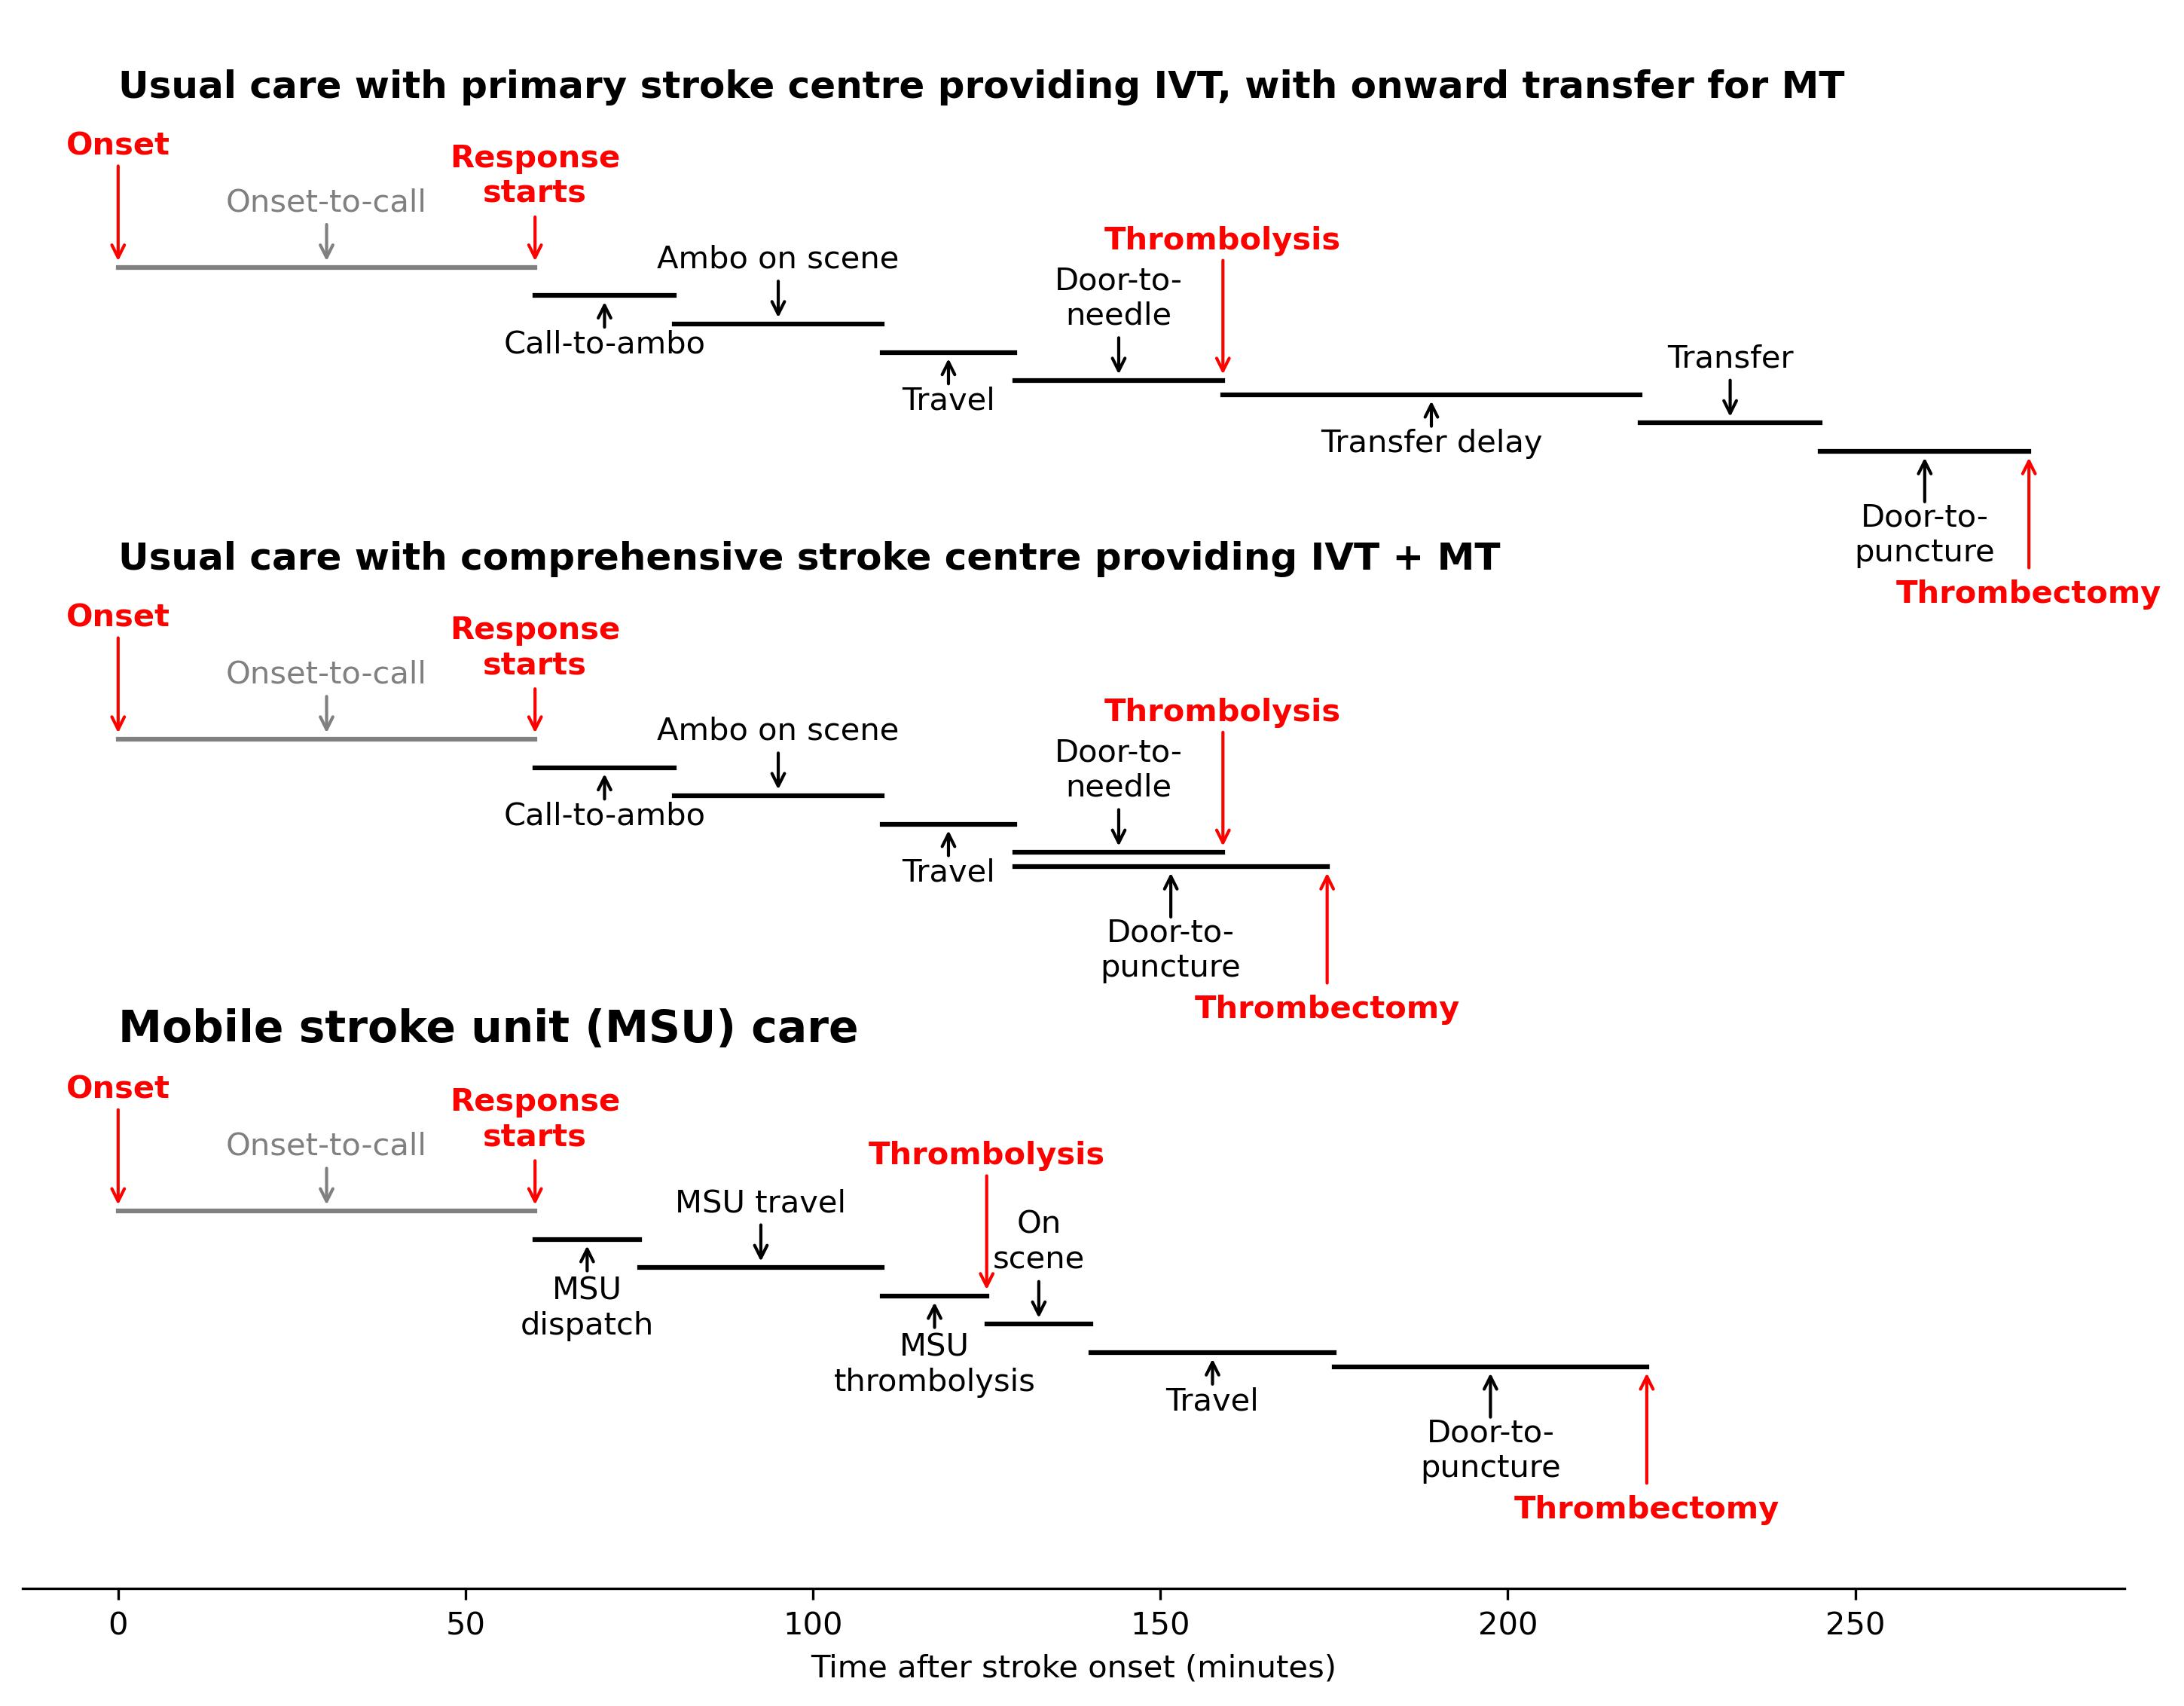
\includegraphics[width=0.85\linewidth]{images/stroke_treatment.jpg}
    \caption{An illustrative timeline showing processes included in the three pathway that are modelled for provision of IVT and MT. Top: Usual care pathway for patients with a PSC closest to their home LSOA, with the PSC providing IVT, followed by the LVO patients having a transfer to the nearest CSC for MT. Middle: Usual care pathway for patients with a CSC closest to their home LSOA, with the CSC providing both IVT and MT. Bottom: The care with MSU pathway, with IVT provided on-scene by the MSU, followed by transfer for LVO patients to the nearest CSC for MT. Process times other than travel times are common for all patients (defined by the scenario). Travel times depend on locations of patient and hospitals, with results calculated for all LSOAs in England.}
    \label{fig:process}
\end{figure}

For each LSOA, times to IVT and MT are calculated by summing all the non-travel process times (common for all patients) and adding required travel times (bespoke for each LSOA location, and for each inter-hospital transfer). The next section will describe how patient outcomes are calculated based on these LSOA-specific times to IVT and MT for usual care or MSU care. All calculations are performed in Python/NumPy.

\subsection{Outcome modelling}

Detailed methods and code used for modelling these outcomes are available at \url{https://github.com/samuel-book/stroke_outcome/}, with methods described as an online book (\url{https://samuel-book.github.io/stroke_outcome/intro.html}). The outcome model is available as a PyPI package for Python (\url{https://pypi.org/project/stroke-outcome/)}.

We used modified Rankin Scale (mRS) as a measure of outcome. mRS is the most commonly used instrument to describe post-stroke functional outcome \cite{quinn_functional_2009}, describing independence of living from a scale of 0 (no disability) through to 5 (severe disability requiring constant nursing attention), with death assigned an mRS of 6. A commonly used surrogate for independent living is  mRS 0-2. Health utility values for each mRS level were taken from Wang \textit{et al.} \cite{wang_utility-weighted_2020}. The mean mRS score, mean utility and proportion of patients with mRS 0-2 in a given mRS distribution can be compared between scenarios.

We calculated the patients mRS outcome distribution based on time to treatment for three patient-treatment cohorts: nLVO treated with IVT; LVO treated with IVT; and LVO treated with IVT + MT. For each patient-treatment cohort we calculated an mRS distribution for treatment at any given time by interpolating between the mRS distribution for treatment given at \emph{t=0} (time of stroke onset) and the mRS distribution for treatment given at \emph{t=No Effect} (time of no effect of treatment), assuming that log odds fall linearly over time \cite{emberson_effect_2014, fransen_time_2016}. Further details on how these \emph{t=No Effect} and \emph{t=No Effect}  were derived are given in the supplementary material.

The time to no effect was 6.3 hours for IVT \cite{emberson_effect_2014} and 8.0 hours for MT \cite{ fransen_time_2016} (our model did not include selection of patients who may still benefit from treatment beyond these durations through the use of perfusion scanning. This number is small for IVT, but is more substantial for MT – approximately 2500 per annum in England. 

Our model did not include selection of patients who may still benefit from treatment beyond these durations 

\subsection{Scenario analysis}

Scenario analysis was undertaken to investigate how changing assumed model parameters (the process durations, in minutes) affect outcomes across all LSOAs. The parameter values were varied according to the following, with all combinations modelled:

\begin{minipage}{1.0\textwidth}  % Define the width of the minipage
\begin{spacing}{1.2}
\begin{itemize}
    \item All patients:
    \begin{itemize}
        \item Stroke onset to call: 0, 60, 120, 180
    \end{itemize}
    \item Usual care:
    \begin{itemize}
        \item Call to ambulance arrival: 15, 30, 45
        \item Ambulance on-scene: 20, 30, 45
        \item Hospital arrival to IVT: 30, 45
        \item Transfer-related delay (excluding travel time): 30, 60, 90
        \item Hospital arrival to MT: 60, 90, 120
    \end{itemize}
    \item Mobile stroke units:
    \begin{itemize}
        \item Call to MSU dispatch: 0, 15, 30, 45
        \item MSU arrival to IVT: 15, 30, 45
        \item MSU on-scene post-IVT: 5, 15
        \item MSU hospital arrival to MT: 30, 60, 90
    \end{itemize}
\end{itemize}
\end{spacing}
\end{minipage}

When onward transfer for MT is required, time to MT at the CSC is often likely to be shorter than time to MT for patients directly admitted to the CSC. This is accounted for in the \textit{net delay} parameter; for example if the \textit{door-in-door-out} time at the first admitting hospital is 90 minutes, but the hospital \textit{arrival-to-MT} is reduced by 30 minutes at the CSC, this is represented as a \textit{net delay} in MT of 60 minutes + transfer travel time.


\subsection{Geographic analysis}

To study geographic variation in benefit of MSUs, a single set of parameters was chosen, reflecting a reasonable base case for performance of usual care and MSU care. Process times (minutes) are shown below, with ambulance and MSU travel times and inter-hospital travel times dependent on patient location (LSOA). In this base case scenario MSUs are based at comprehensive stroke centres only. 

\begin{minipage}{1.0\textwidth}  % Define the width of the minipage
\begin{spacing}{1.2}
\begin{itemize}
    \item All patients:
    \begin{itemize}
        \item Stroke onset to call: 60
    \end{itemize}
    \item Usual care:
    \begin{itemize}
        \item Call to ambulance arrival: 20
        \item Ambulance on-scene: 30
        \item Hospital arrival to IVT: 45
        \item Transfer-related delay (excluding travel time): 60
        \item Hospital arrival to MT: 90
    \end{itemize}
    \item Mobile stroke units:
    \begin{itemize}
        \item Call to MSU dispatch: 15
        \item MSU arrival to IVT: 30
        \item MSU on-scene post-IVT: 5
        \item MSU hospital arrival to MT: 60
    \end{itemize}
\end{itemize}
\end{spacing}
\end{minipage}


\subsection{Varying number of MSU base locations}

In order to study the effect of changing the number of MSU base locations, a greedy algorithm was used. In this method, 100 MSU base locations are sequentially added, with each additional one chosen only from the CSCs, in the order of maximum improvement in outcomes (utility). The utility gain is calculated for those patients treated by an MSU rather than usual care; the algorithm is therefore looking at the effect of changing the number of MSU base locations, rather than the number of physical MSUs. The algorithm can also be run with MSUs chosen from any stroke unit type.
\section{Results}

\subsection{Scenario analysis}

Figure \ref{fig:scenarios_overview} shows the range of results, measured by utility or the proportion of patients with an outcome of mRS 0-2, separating the changes for nLVO and LVO. Across all scenarios MSUs are usually found to be advantageous compared with usual care, but in some scenarios (comparing the best likely usual care with the worst likely MSU care), MSUs were found to be disadvantageous compared with usual care. Across the majority of scenarios the benefit of MSU care over usual care was typically (interquartile range across scenarios) an improvement of 0.005 to 0.021 in utility for nLVO, and 0.016-0.052 for LVO treated with both IVT and MT. This translated to an improvement of the proportion of patients mRS 0-2 of 0.005-0.023 for nLVO, and 0.017-0.055 for LVO treated with both IVT and MT. The benefit to patients with LVO was derived mostly by improving benefit of MT by direct transport to a MT-capable unit. For the combined nLVO/LVO population (assuming 70\% nLVO and 30\%LVO in the treated population) there was typically (interquartile range across scenarios) an improvement of 0.010-0.029 in utility, and improvement of the proportion of patients mRS 0-2 of 0.011-0.032.


\begin{figure}[h!]
    \centering
    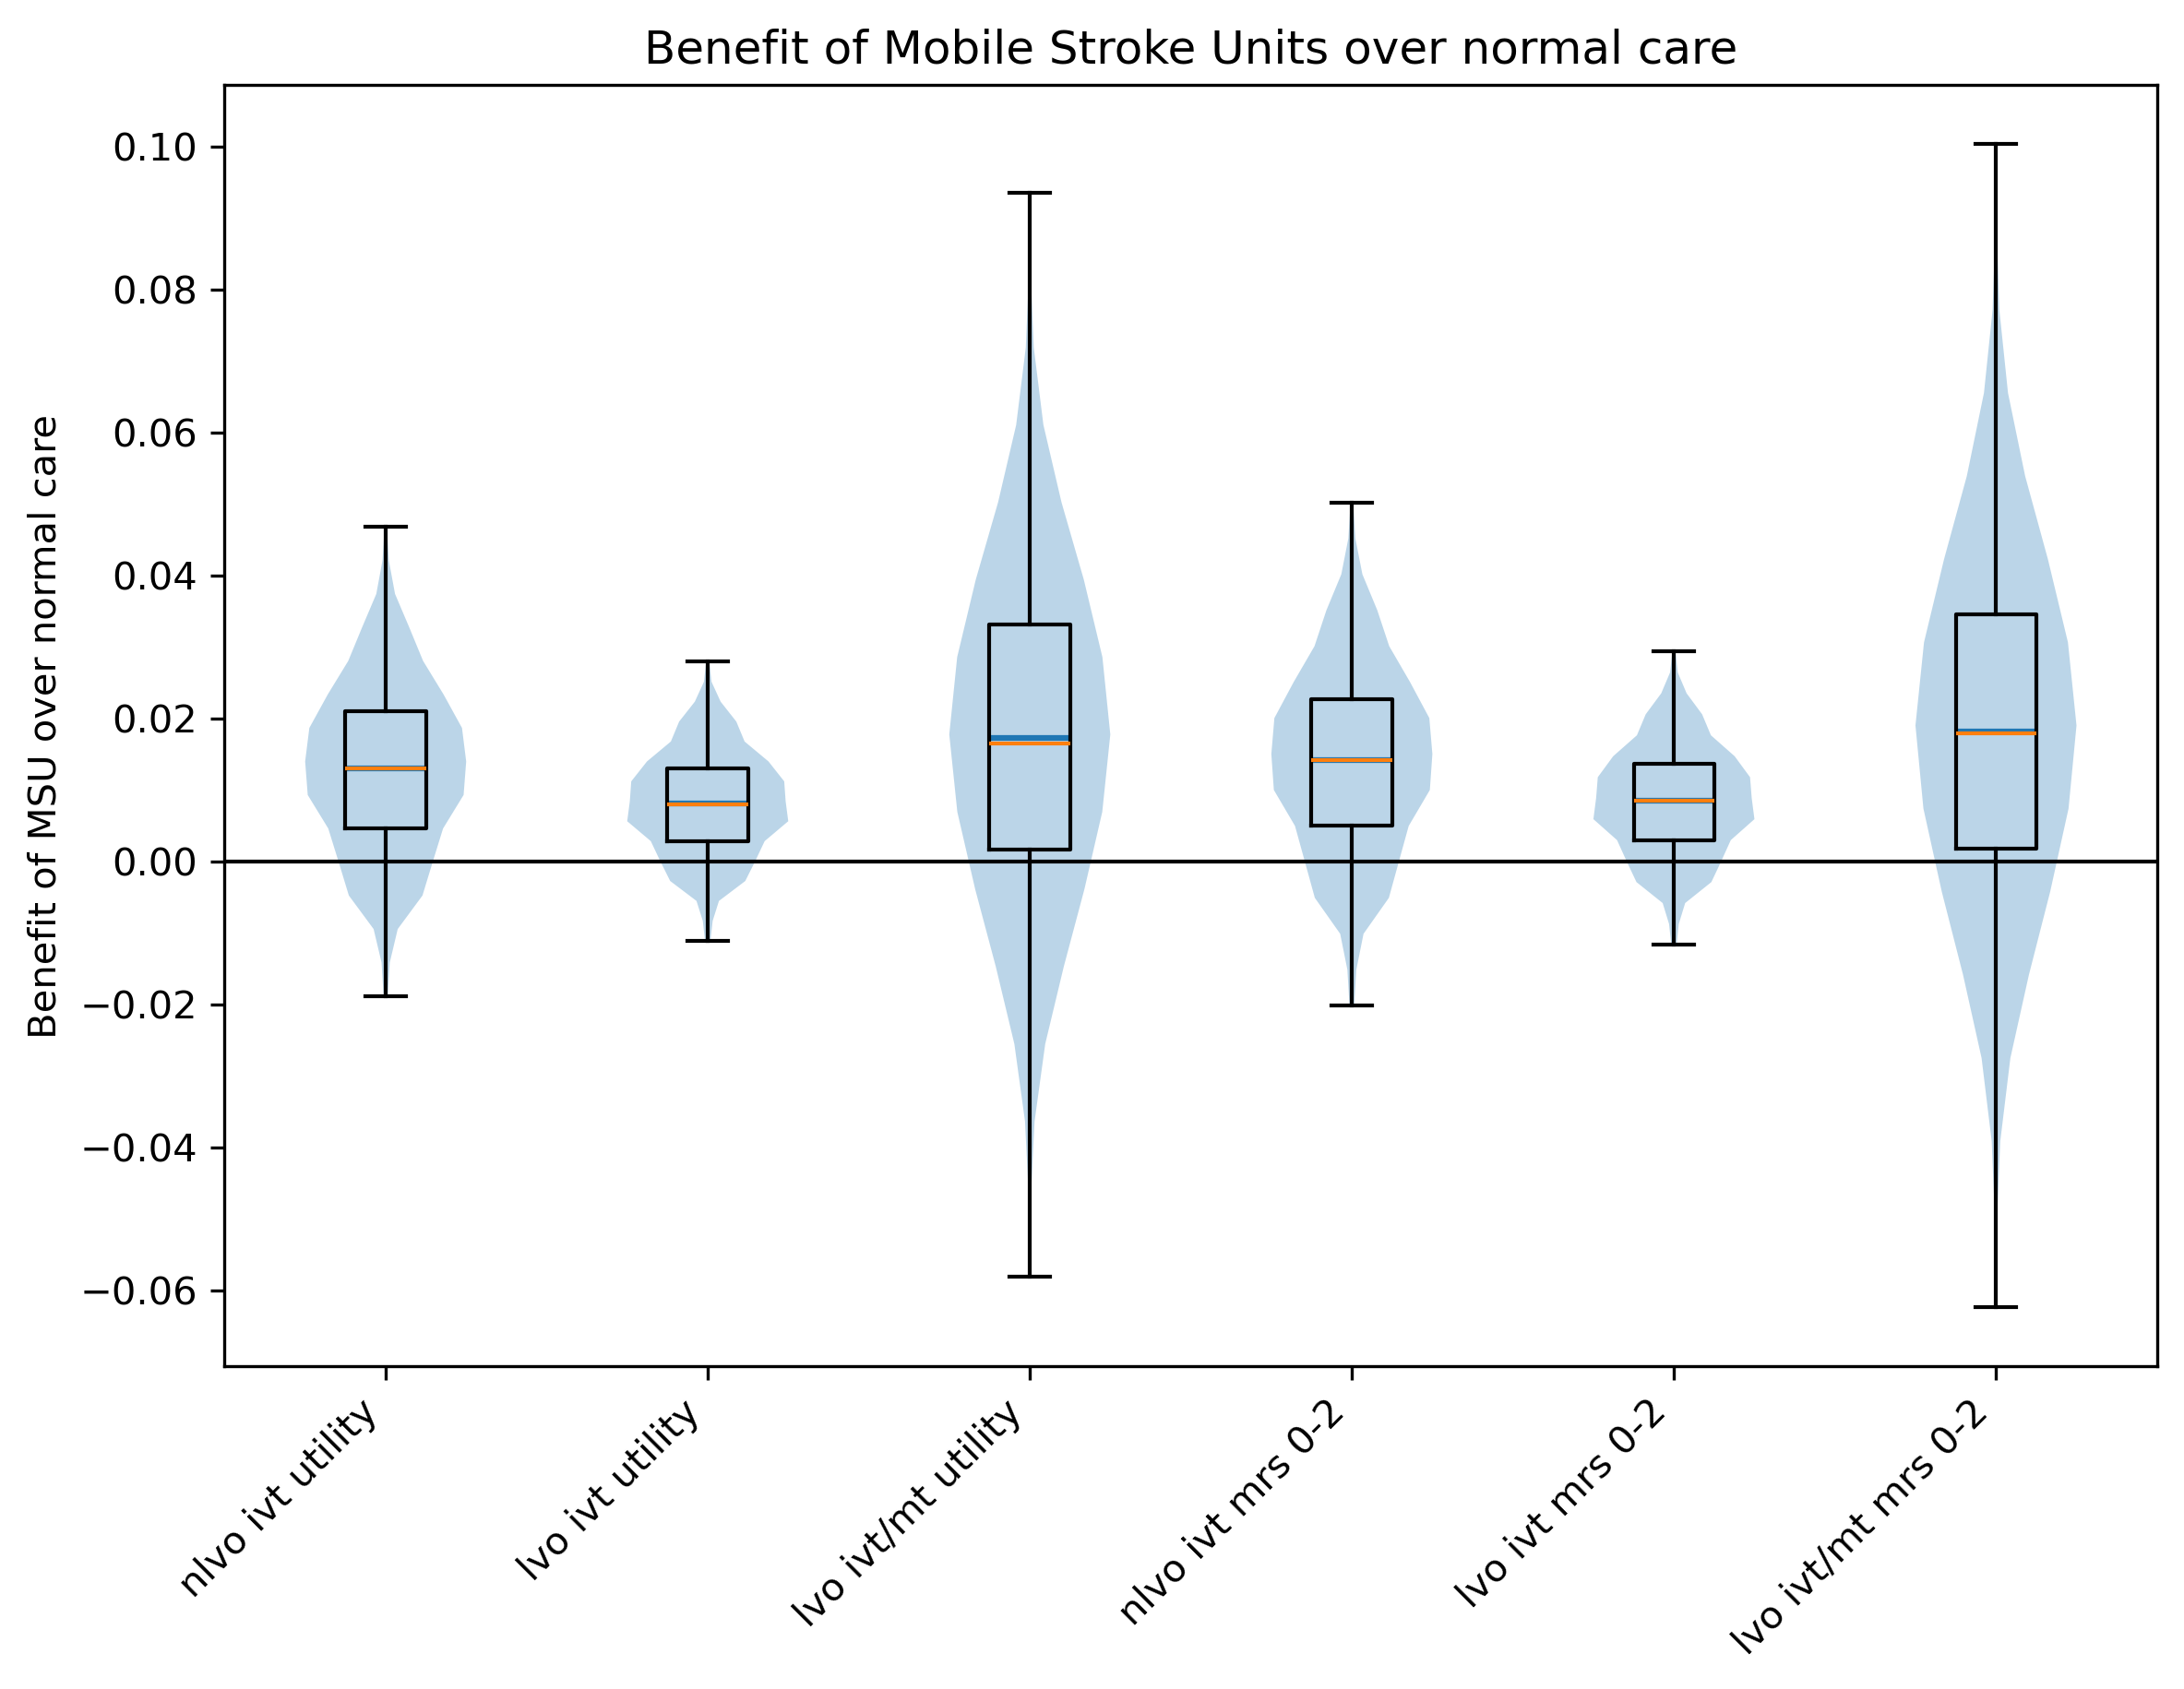
\includegraphics[width=0.6\linewidth]{images/scenario_results_summary.png}
    \caption{Benefit of usual care over MSU care across all scenarios, in the treated population, measured by utility or the proportion of patients with an outcome of mRS0-2, separating the changes for nLVO and LVO. Results for LVO show the effect of MSUs on the benefit derived from IVT alone, or by IVT/MT in combination. Box plots show range, interquartile range, and median. The combined nLVO/LVO benefit assumed 70\% nLVO and 30\%LVO in the treated population. Overlaid over the box plots are violin plots showing the distribution of results across all scenarios. A positive value indicates MSUs provide an advantage over usual care, and a negative result show MSUs are disadvantageous compared with usual care. Results are the average effect across all LSOAs in England.}
    \label{fig:scenarios_overview}
\end{figure}



Figure \ref{fig:scenarios_utility} shows how changing model parameters affects the predicted benefit of MSUs, using utility as a measure. Results show the combined affect on nLVO/LVO assuming 70\% nLVO and 30\% LVO  in the treatable population. Changing time from onset to call only had marginal effect on the benefit of MSUs over usual care. Changing parameters that worsen usual care (such as lengthening ambulance response times, or lengthening arrival to IVT, lead to improved advantages of MSUs over usual care. Likewise, changing parameters that improve MSU care (such as MSU dispatch times, or time to IVT on scene) improved advantages of MSUs over usual care.

\begin{figure}[h!]
    \centering
    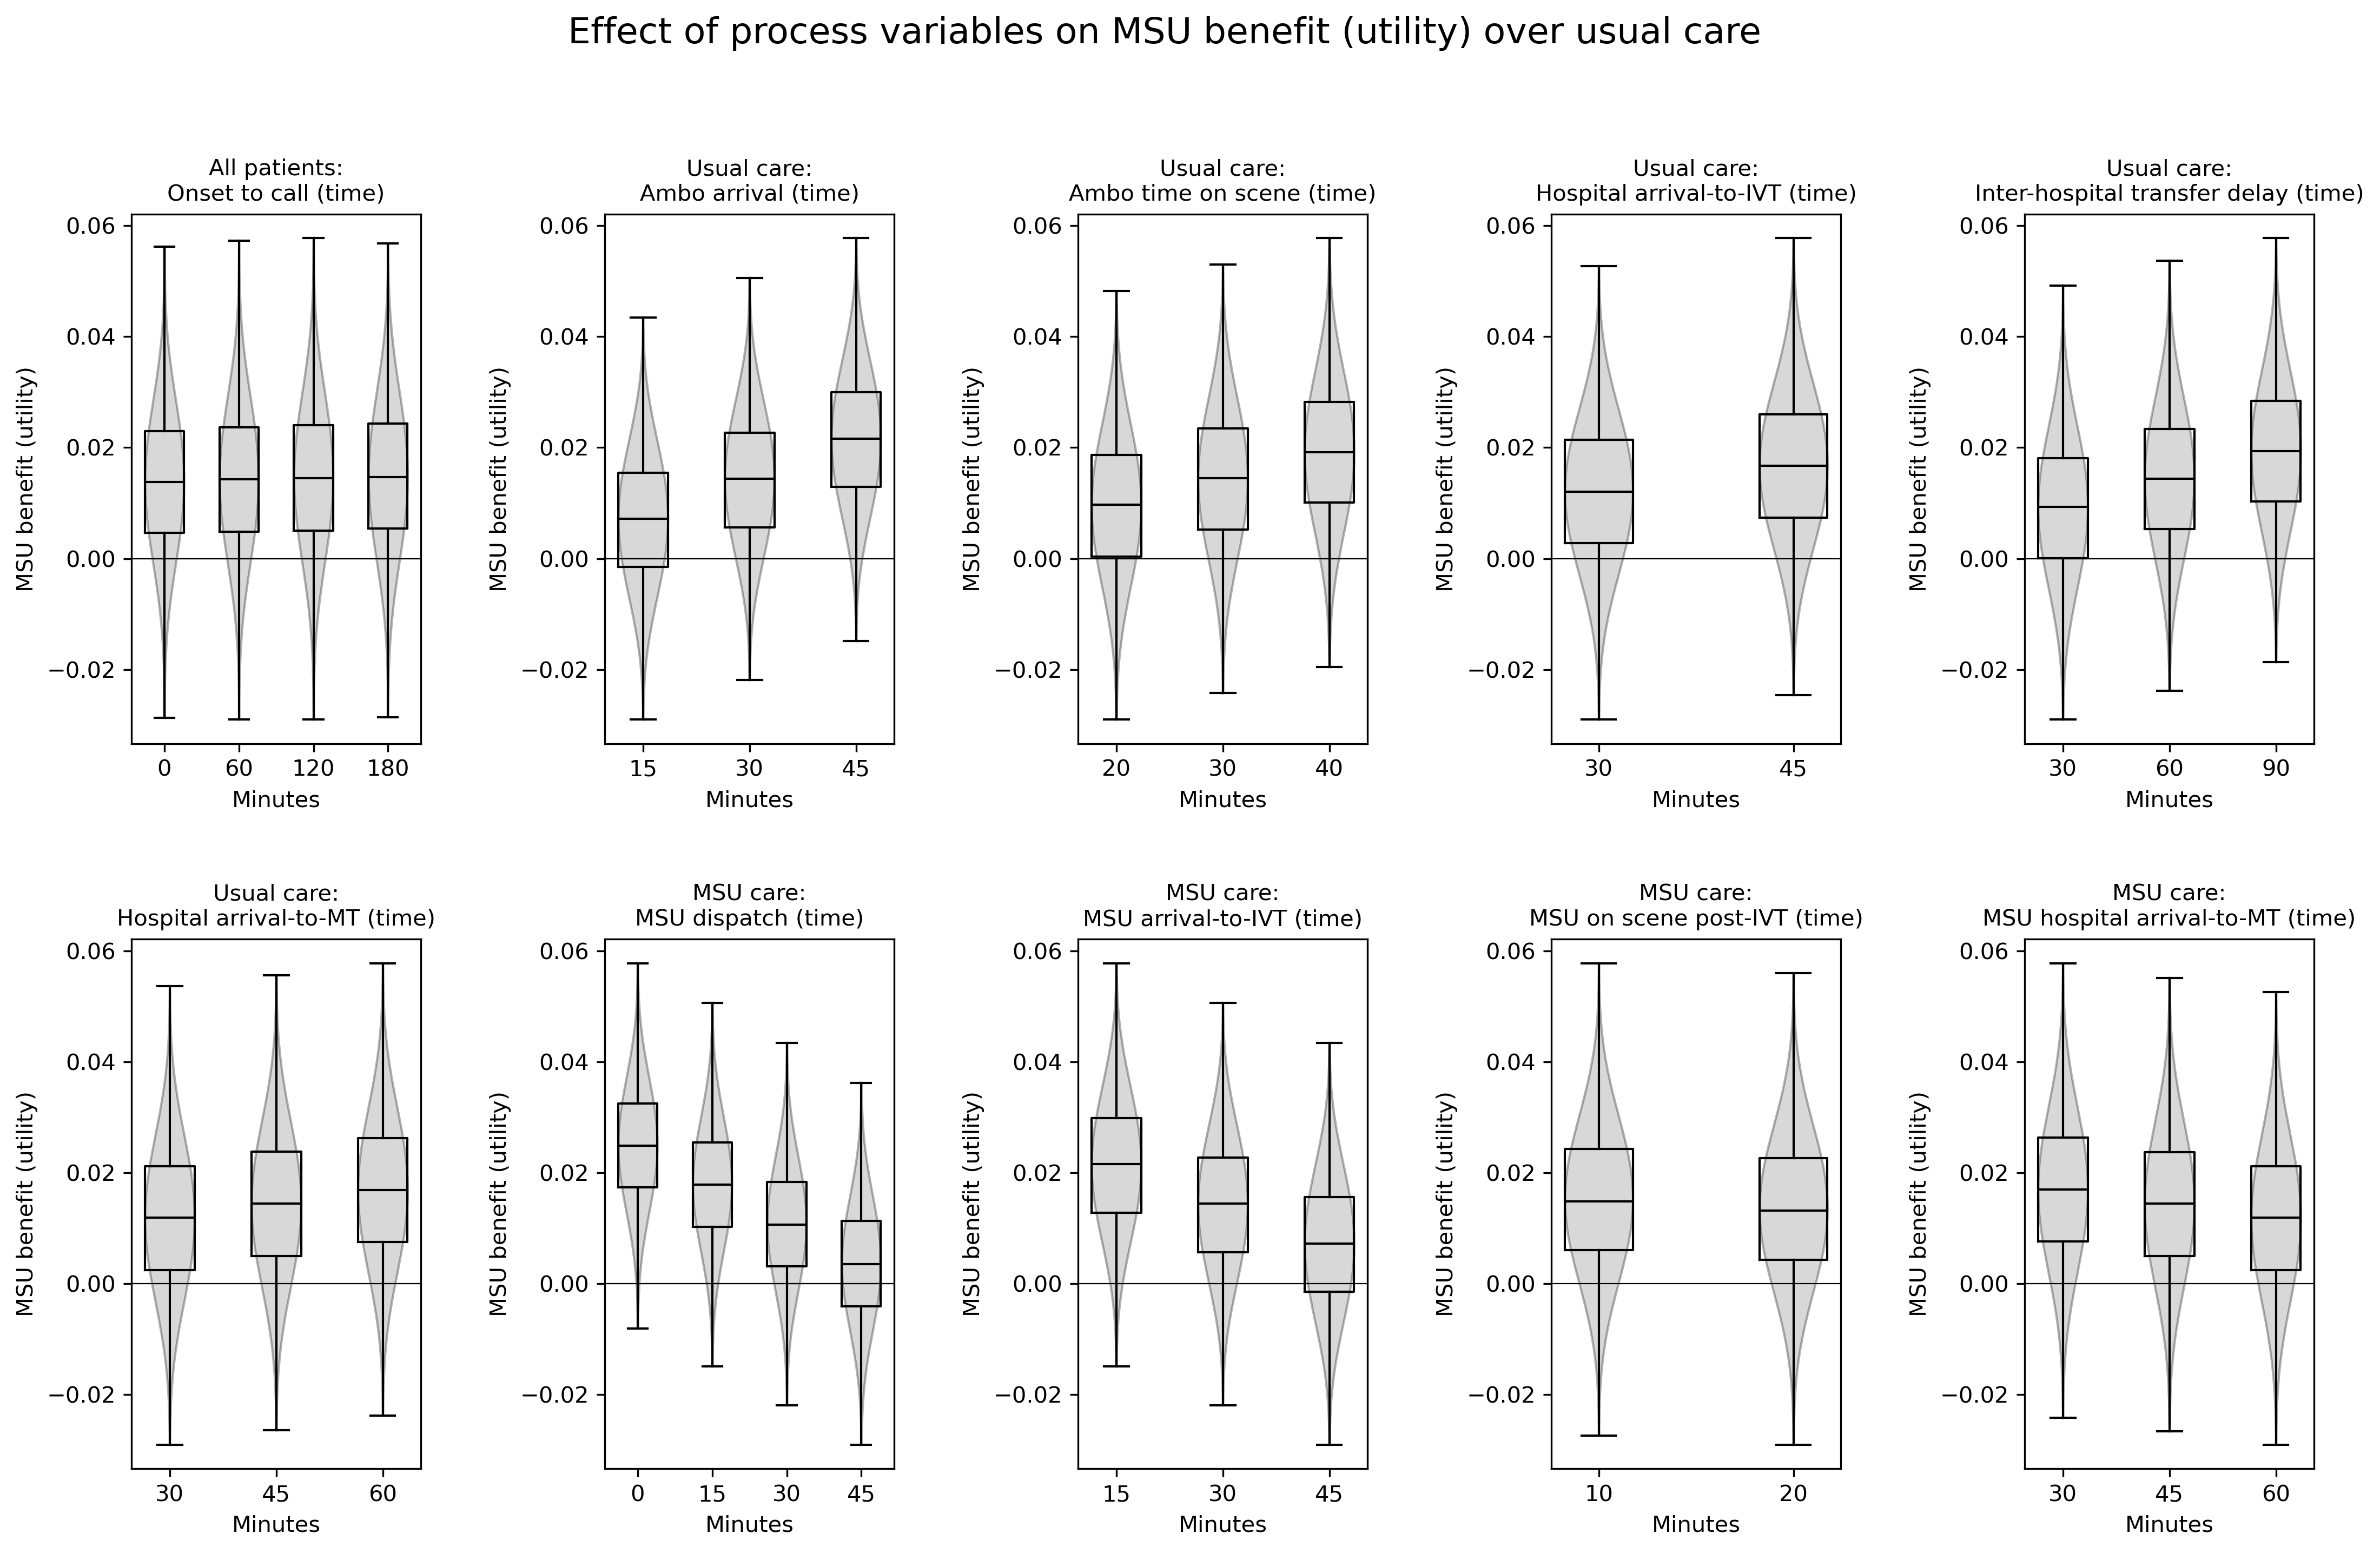
\includegraphics[width=1\linewidth]{images/msu_net_utility_benefit.png}
    \caption{The effect of changing model parameters on the predicted benefit of MSUs over usual care, in the treated population, measured by utility. For each target parameter results are averaged across all scenarios with that given parameter value. Box plots show range, interquartile range, and median. Overlaid over the box plots are violin plots showing the distribution of results across all scenarios. Results are the average effect across all LSOAs in England.}
    \label{fig:scenarios_utility}
\end{figure}

\subsection{Geographic variation}

In the base case scenario MSUs are based at comprehensive stroke centres only, and we assume there is a mix of 70\% nLVO and 30\% LVO in the treated population.

Figure \ref{fig:map_times} shows travel and transfer times for usual care and for MSUs. When a patient first attends an IVT-only centre, the times to IVT include the travel time to the IVT-only centre, the inter-hospital travel time, and a net additional delay of 60 minutes. There is significant variation in travel times to IVT centres, but there is more substantial variation in times to MT due to the need for transfer. 67\% of LSOAs and 70\% of admissions require transfer for MT. As, the base MSUs are based at comprehensive stroke centres only, travel times for a MSU can exceed the travel time of a normal ambulance to the closest centre providing IVT, and this extra travel time can lead to delayed time to IVT in those regions furthest away from MSU bases locations.

\begin{figure}[h!]
    \centering
    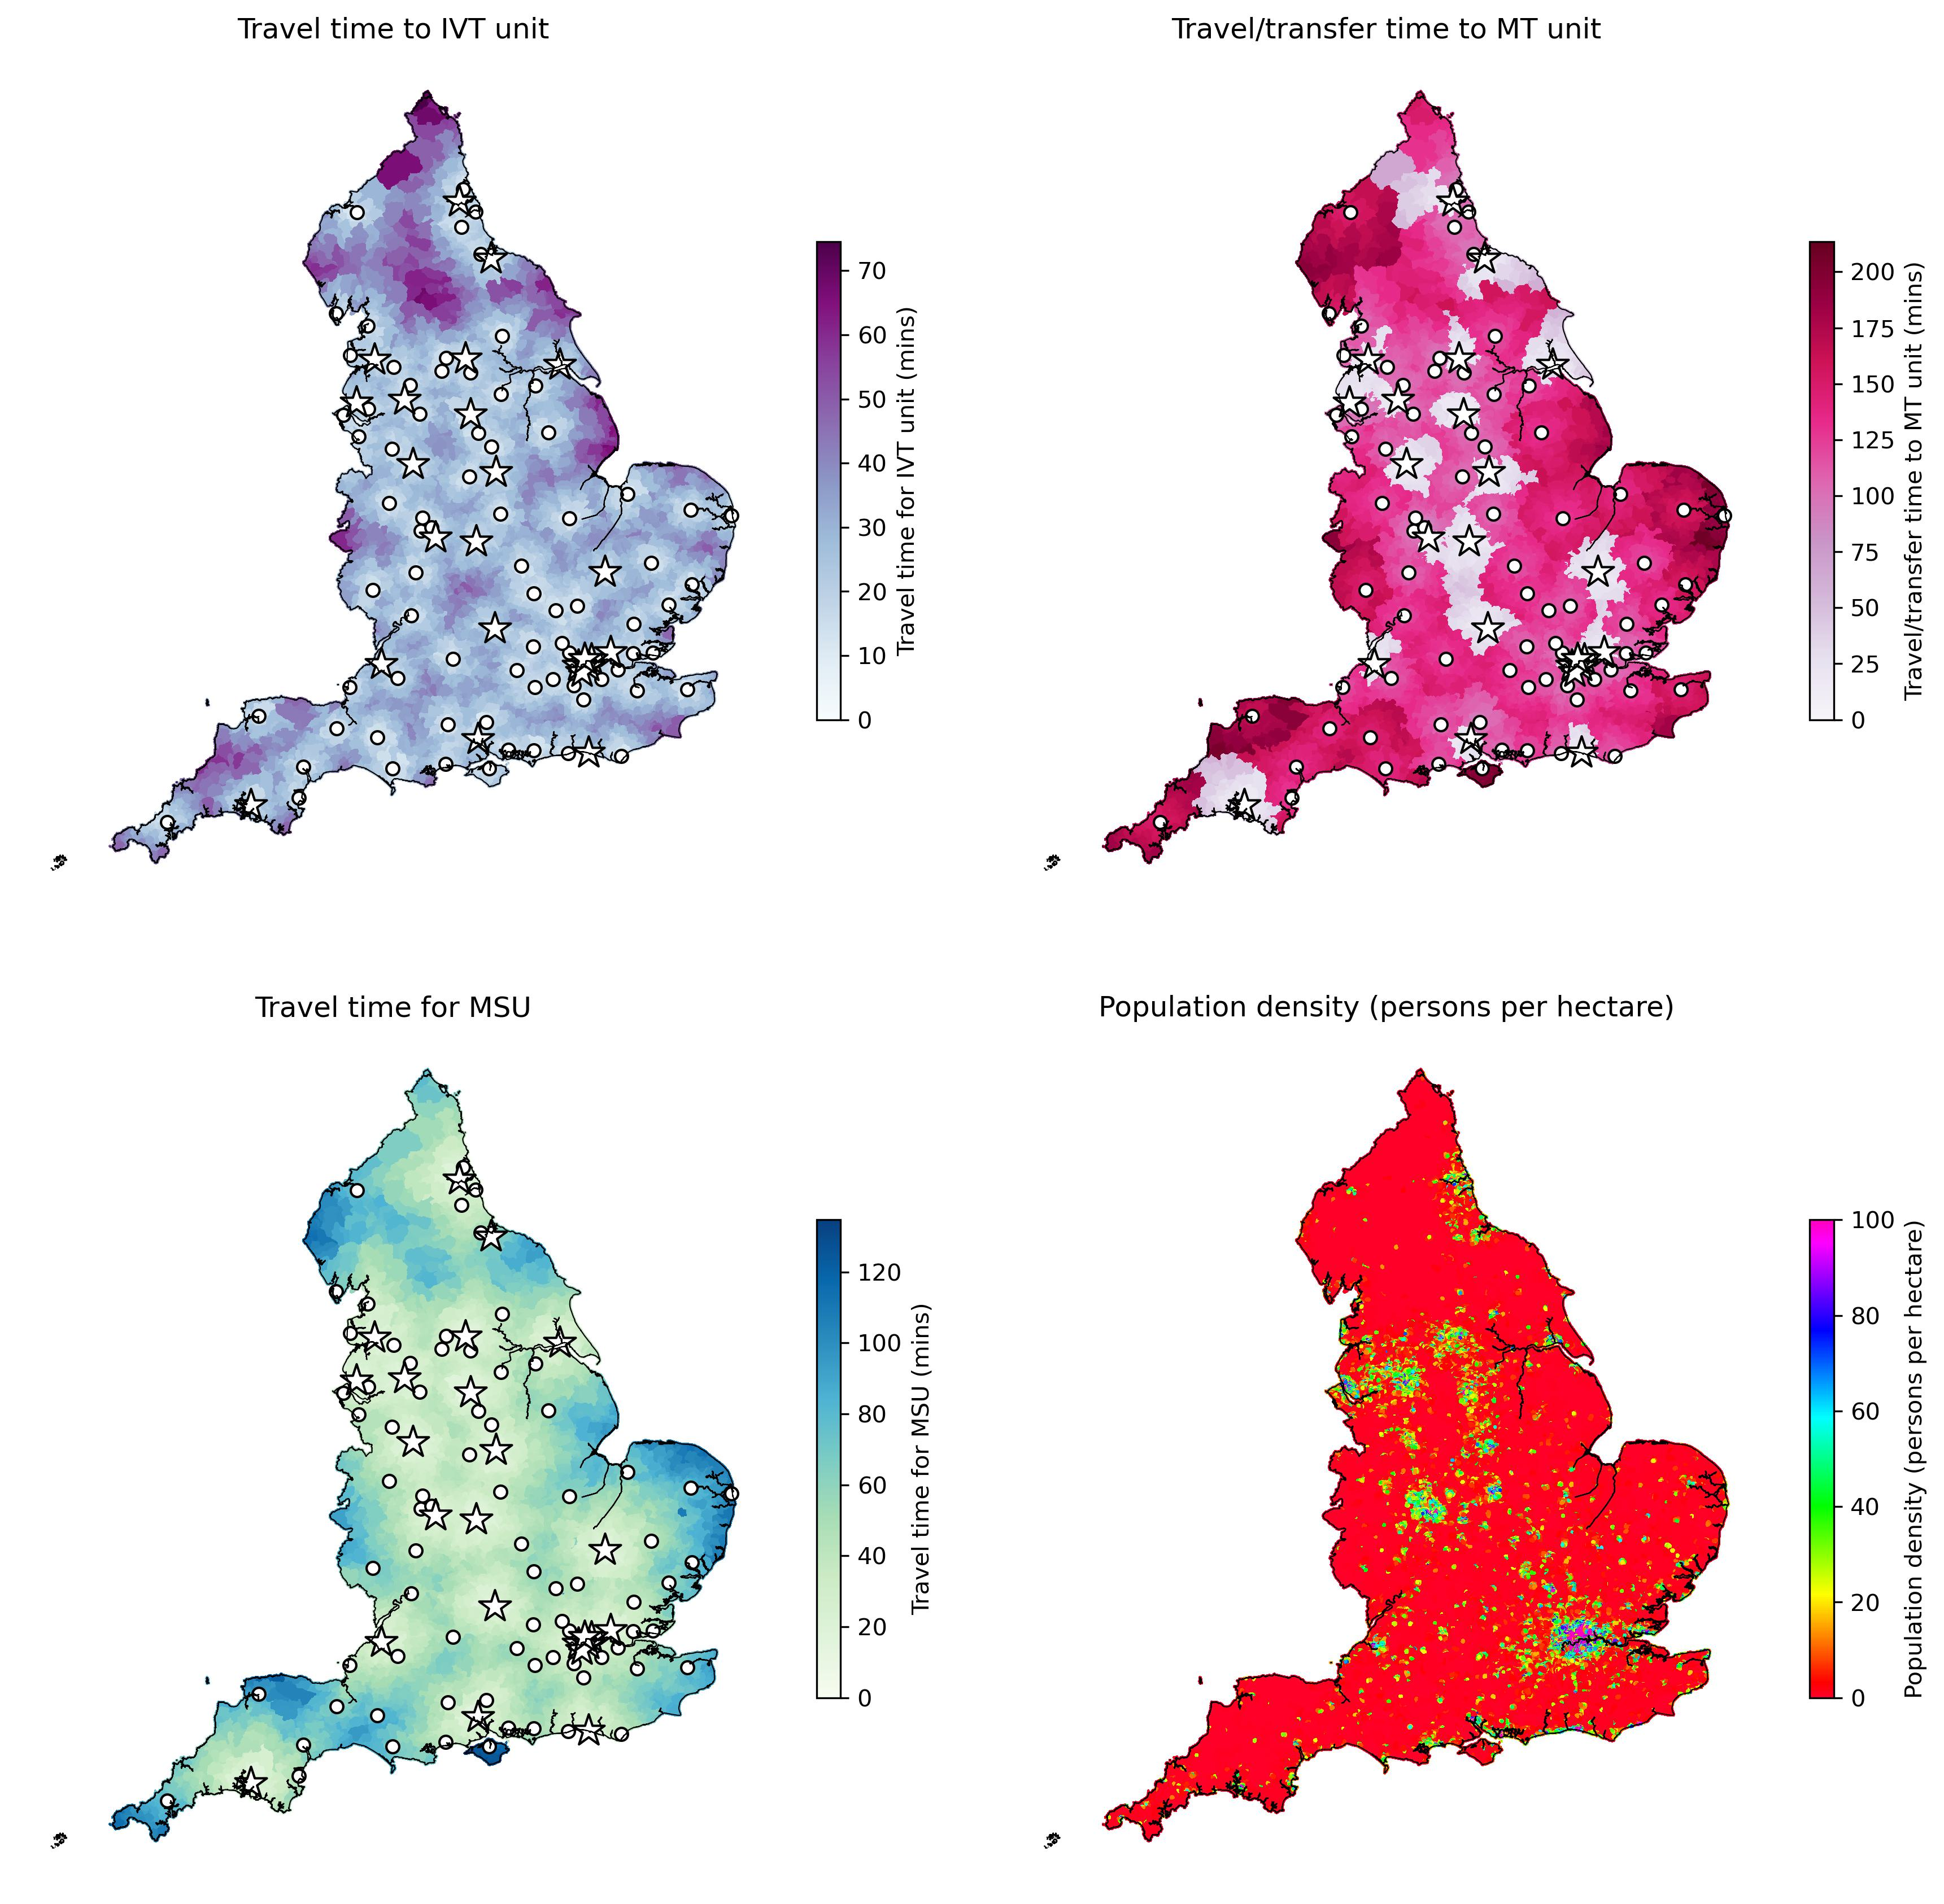
\includegraphics[width=1.0\linewidth]{images/map_times.jpg}
    \caption{Travel times and population density for each LSOA. \textit{Top left}: Travel times to nearest unit providing IVT. \textit{Top right}: Travel times to unit providing MT. For those first attending an IVT-only centre, the travel times include the travel time to the IVT-only centre, the inter-hospital travel time, and a net additional delay of 60 minutes. \textit{Bottom left}: Travel times for MSUs. \textit{Bottom right}: Population desnity (with scale capped at 100 persons per hectre). Circles show locations of IVT-only units. Stars show locations of comprehensive stroke centres providing both IVT and MT, and being the base locations of MSUs.}
    \label{fig:map_times}
\end{figure}


In this base case, without reperfusion treatment, there is an average outcome utility of 0.52 across nLVO and LVO. With usual care, the is a utility gain of 0.086 in treated patients. MSUs provided an average further utility gain in treated patients of 0.022 over usual care.

Figure \ref{fig:msu_map_utility} shows maps of geographic variation in benefit of MSUs over usual care, by stroke type, using the reasonable base case scenario. Figure \ref{fig:msu_histograms} shows the distribution of net benefit (assuming 70\%nLVO, 30\% LVO in the treated population) across LSOAs. There is significant variation in the benefit of reperfusion using usual care, with those living closest to comprehensive stroke units receiving the greatest benefit. This is due the larger utility gain of reperfusion treatment coming from the treatment of LVO, and with those patients benefiting most from rapid access to thrombectomy.

The benefit of MSUs over usual care follows different patterns for nLVO and LVO. For nLVO, the benefit of MSU falls with distance away from the MSU base. For LVO the benefit first falls with with distance away from the MSU base, but then benefit increases where use of the MSU avoids inter-hospital transfer for MT, before falling again with greater travel times for the MSU. The catchment area of benefit for LVO, when using MSUs, is therefore wider than the catchment area of benefit for nLVO, with the maximum benefit being in a halo a little way away from the MSU base location, where patient transfer for MT is avoided but MSU travel times are still acceptable.


\begin{figure}[h!]
    \centering
    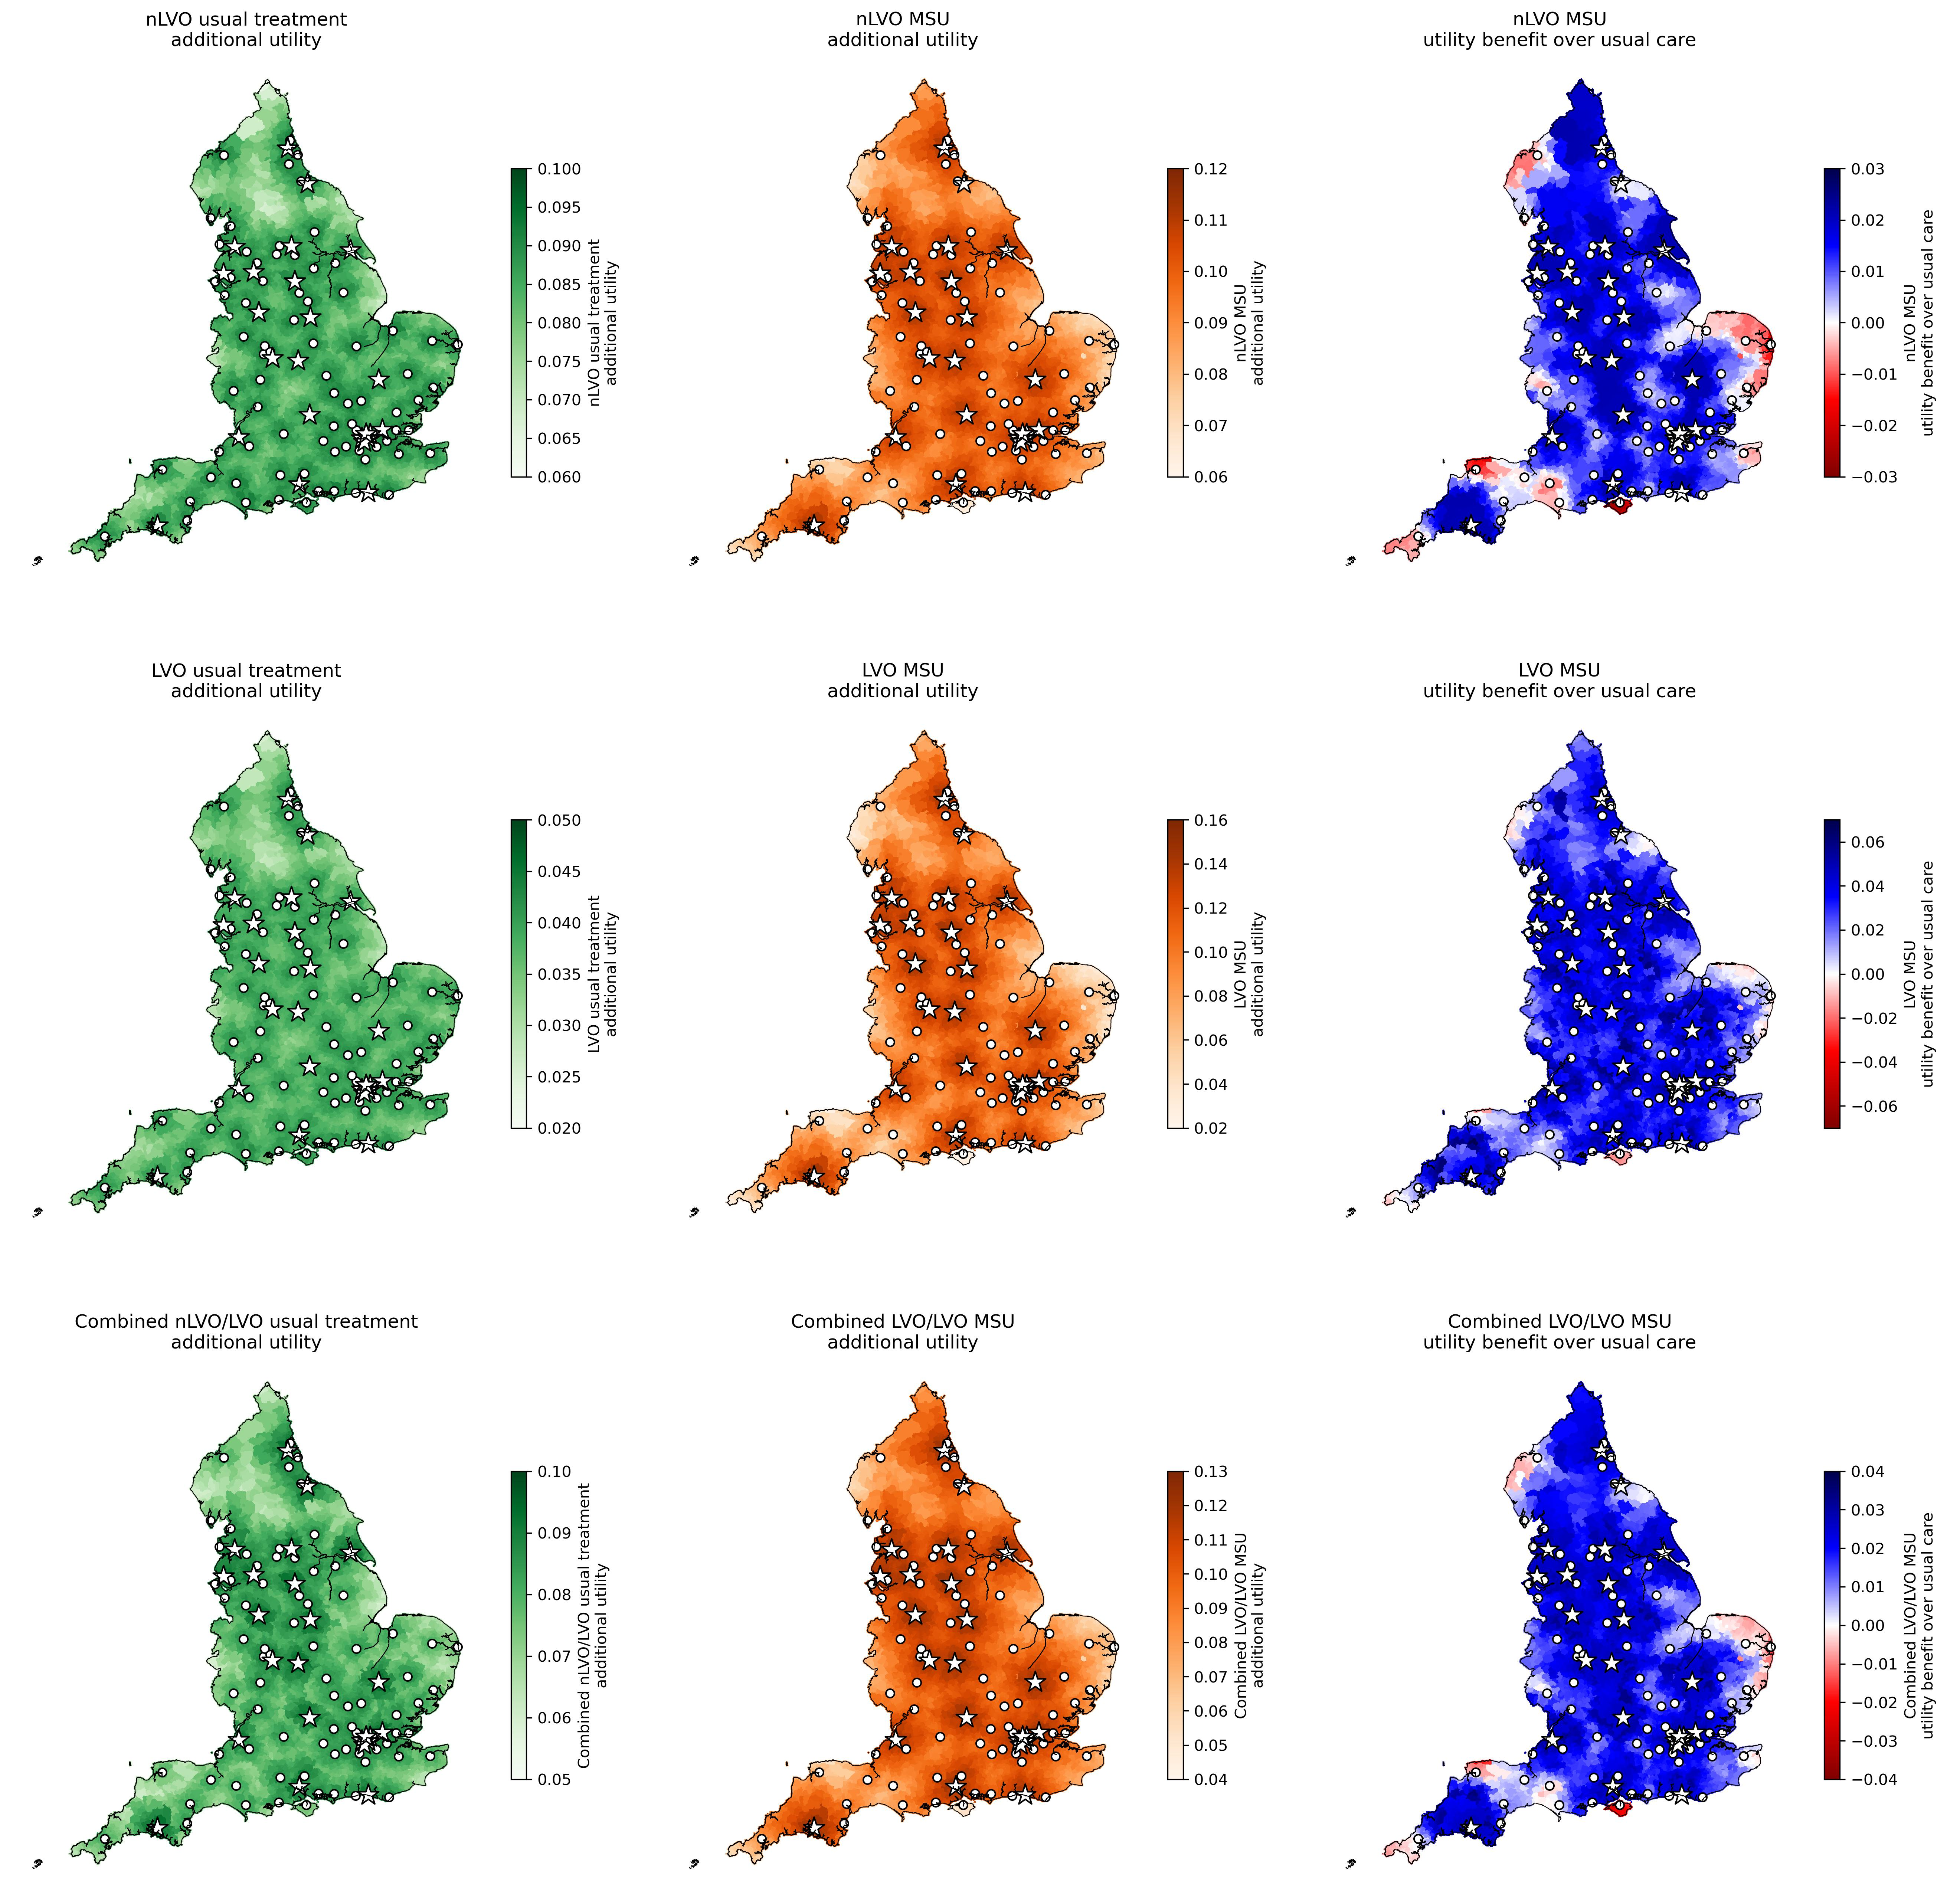
\includegraphics[width=1\linewidth]{images/map_utility.jpg}
    \caption{Map of treatment benefits, calculated by LSOA for the treated population. \textit{Top}: Treatment of nLVO; \textit{Middle}: Treatment of LVO, \textit{Bottom}: Combination of treatment (based on 70\% nLVO and 30\% LVO in the treated population). \textit{Left (green)}: Benefit of usual care over no treatment;\textit{Middle (orange)}: Benefit of MSU care over no treatment; \textit{Right (blue/red)}: Benefit of MSU care over usual care. Circles show locations of IVT-only units. Stars show locations of comprehensive stroke centres providing both IVT and MT, and being the base locations of MSUs.}
    \label{fig:msu_map_utility}
\end{figure}

Figure \ref{fig:msu_histograms} shows histograms of benefit of MSUs over usual care. For most LSOAs MSU improve time to IVT and MT, but some areas have worsened times. This is reflected in most areas having a benefit of about a 0.03 increase in the proportion of patients with MRS 0-2 after stroke, and similarly a benefit of about a 0.03 increase in utility after stroke. Some areas though have reduced benefit, or even disbenefit of using MSUs. The maximum benefit is about 0.04 improvement in both the proportion of patients with MRS 0-2 after stroke and utility after stroke.

\begin{figure}[h]
    \centering
    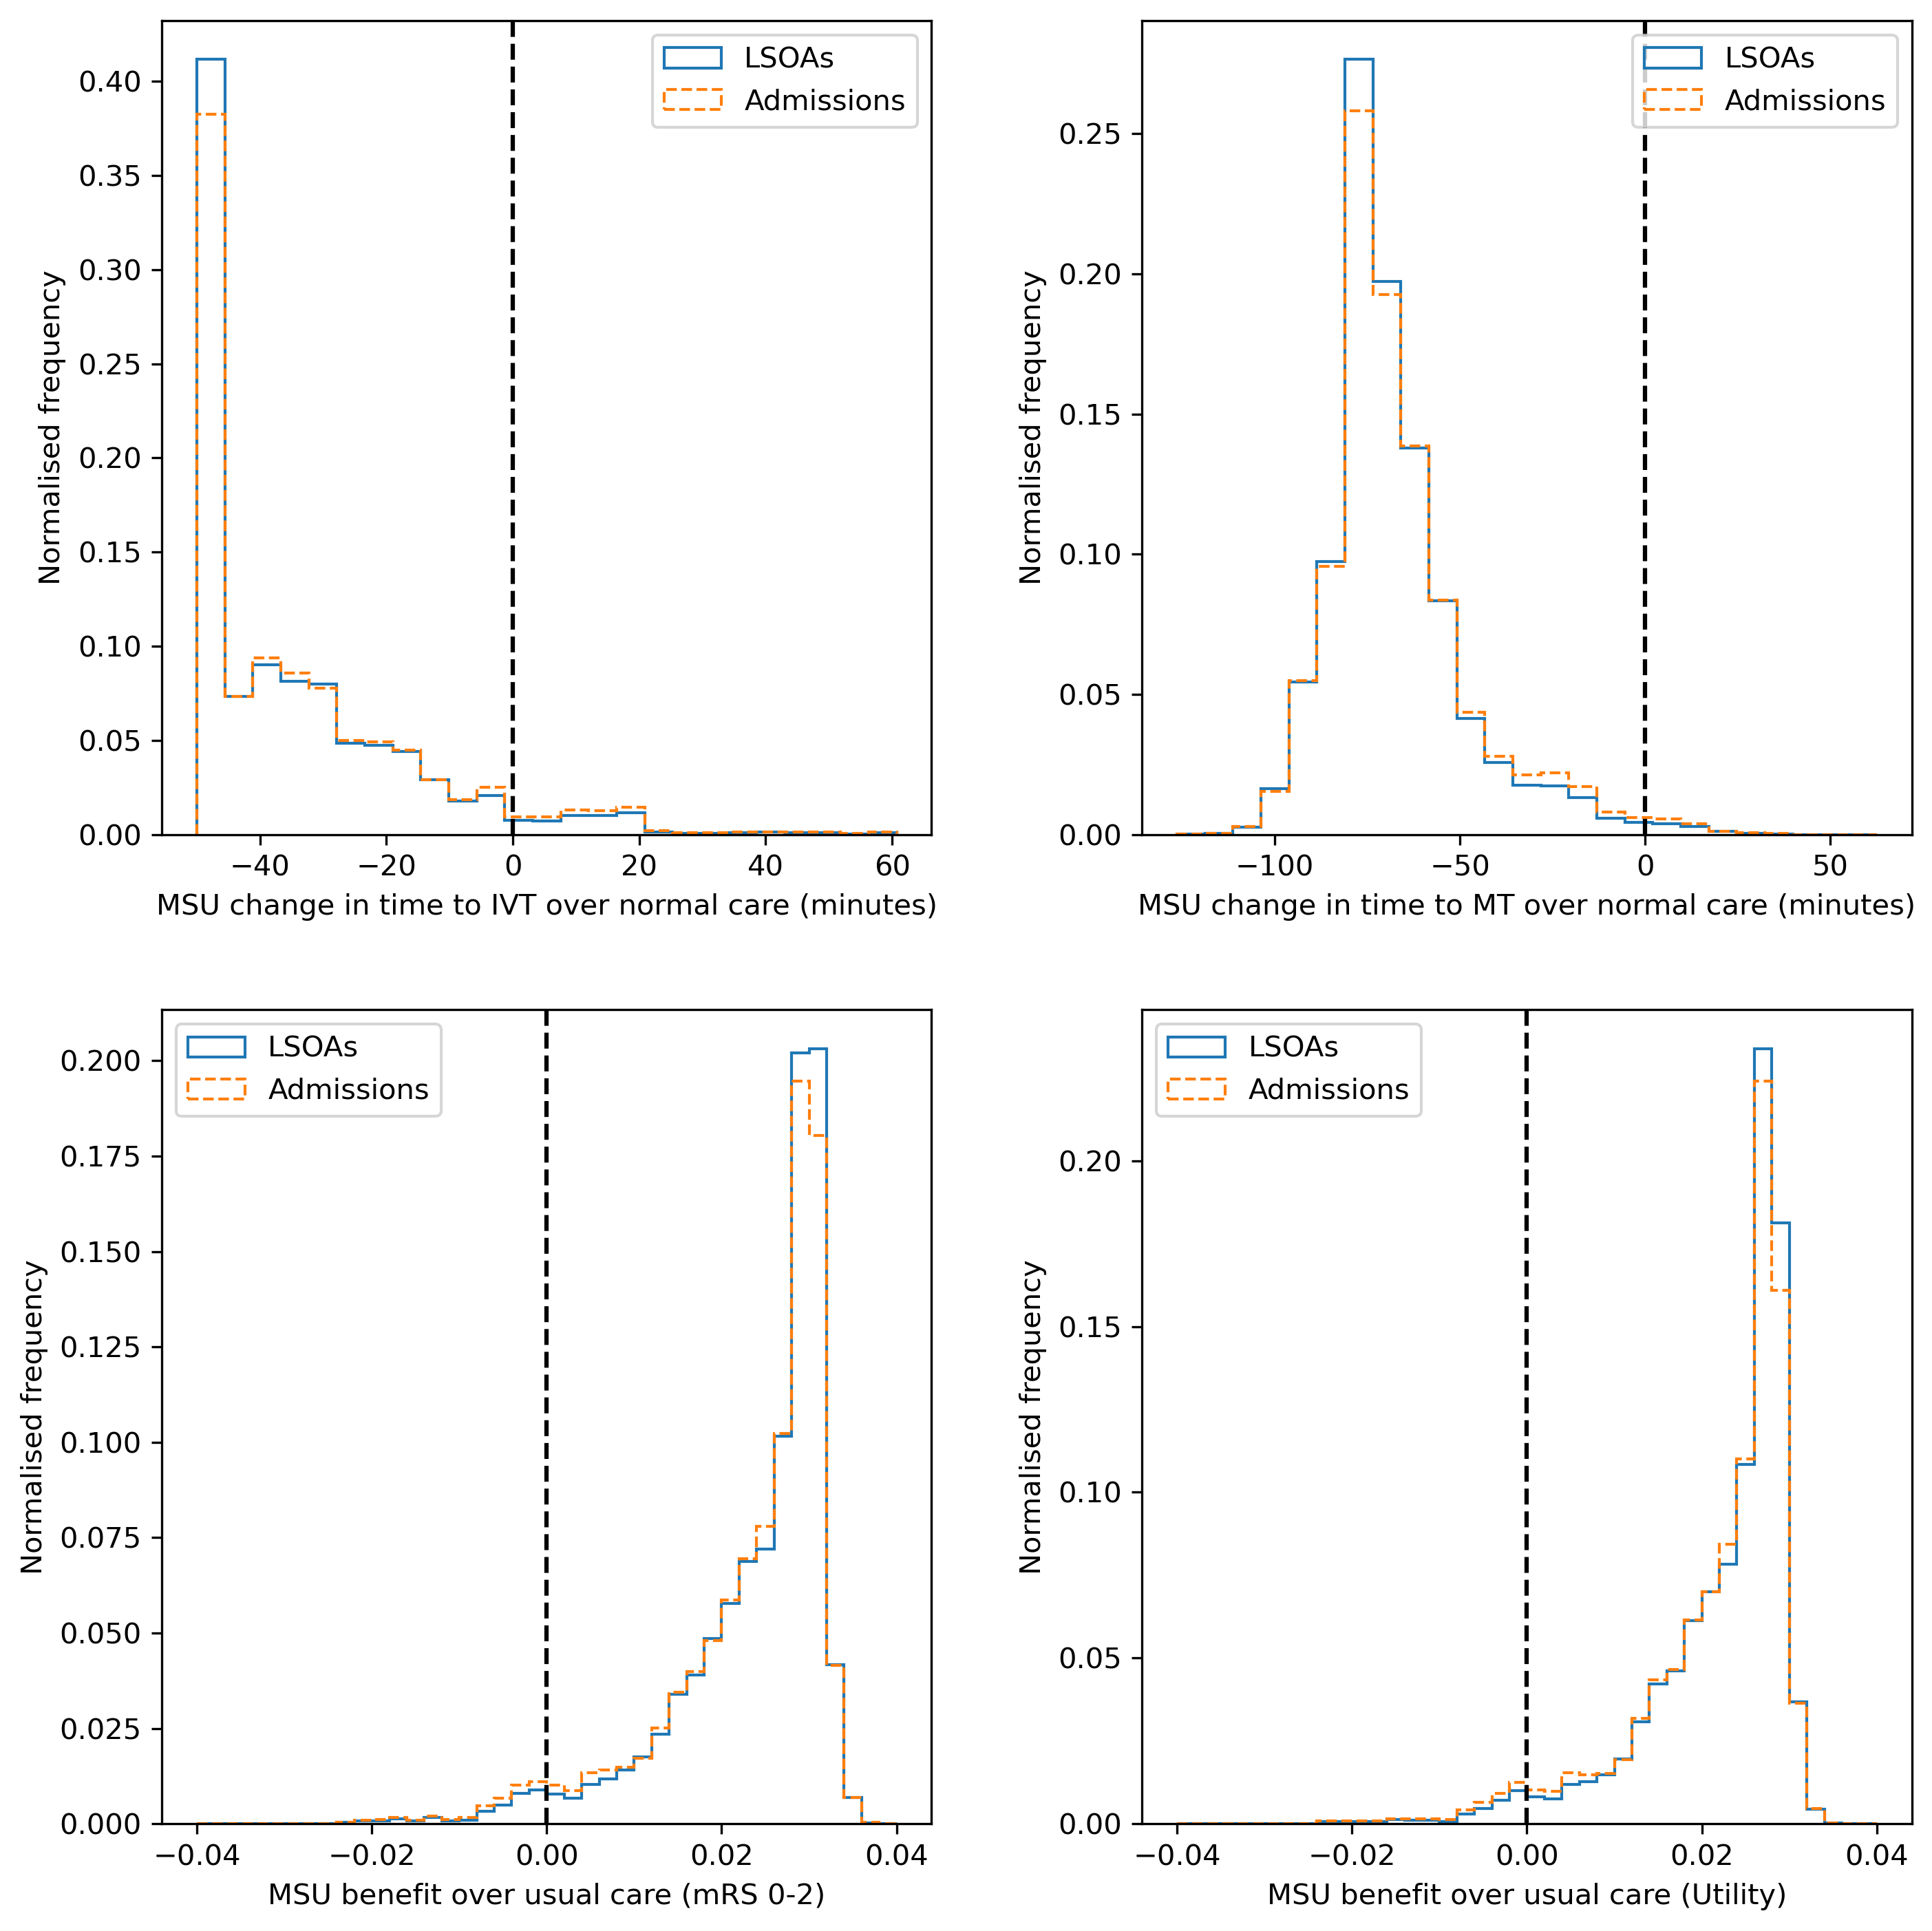
\includegraphics[width=0.75\linewidth]{images/histograms.png}
    \caption{Distribution of benefit of MSUs over normal care across MSUs. Benefit is described either as even across LSOAs (solid line), or weighted by admissions by LSOA (dotted line). Histograms show change in time to IVT (top left), time to MT (top right), proportion mRS 0-2 (bottom left), or utility (bottom right).}
    \label{fig:msu_histograms}
\end{figure}

\subsection{Varying number of MSU locations}

A greedy algorithm was used to select locations of MSUs. The utility gain is calculated for those patients treated by a MSU rather than usual care. As the number of MSU locations increased, the benefit of MSUs over usual care increased (\ref{fig:greedy}), but with diminishing returns. The advantage of MSU care over usual care improved utility by 0.020, 0.024, 0.027, and  with 10, 25, 50 and 100 MSU base locations when MSU locations are chosen from any sttroke unit type. 

When selecting locations of mobile stroke units, in the first 10 selections, 3 were comprehensive stroke units, and in the first 20, 8 were comprehensive stroke units. With MSUs based at 23 current MY centres the net utility benefit over normal care was 0.022. With optimal selection of location of the same number of bases the utility benefit was increased to 0.023.

\begin{figure}[h]
    \centering
    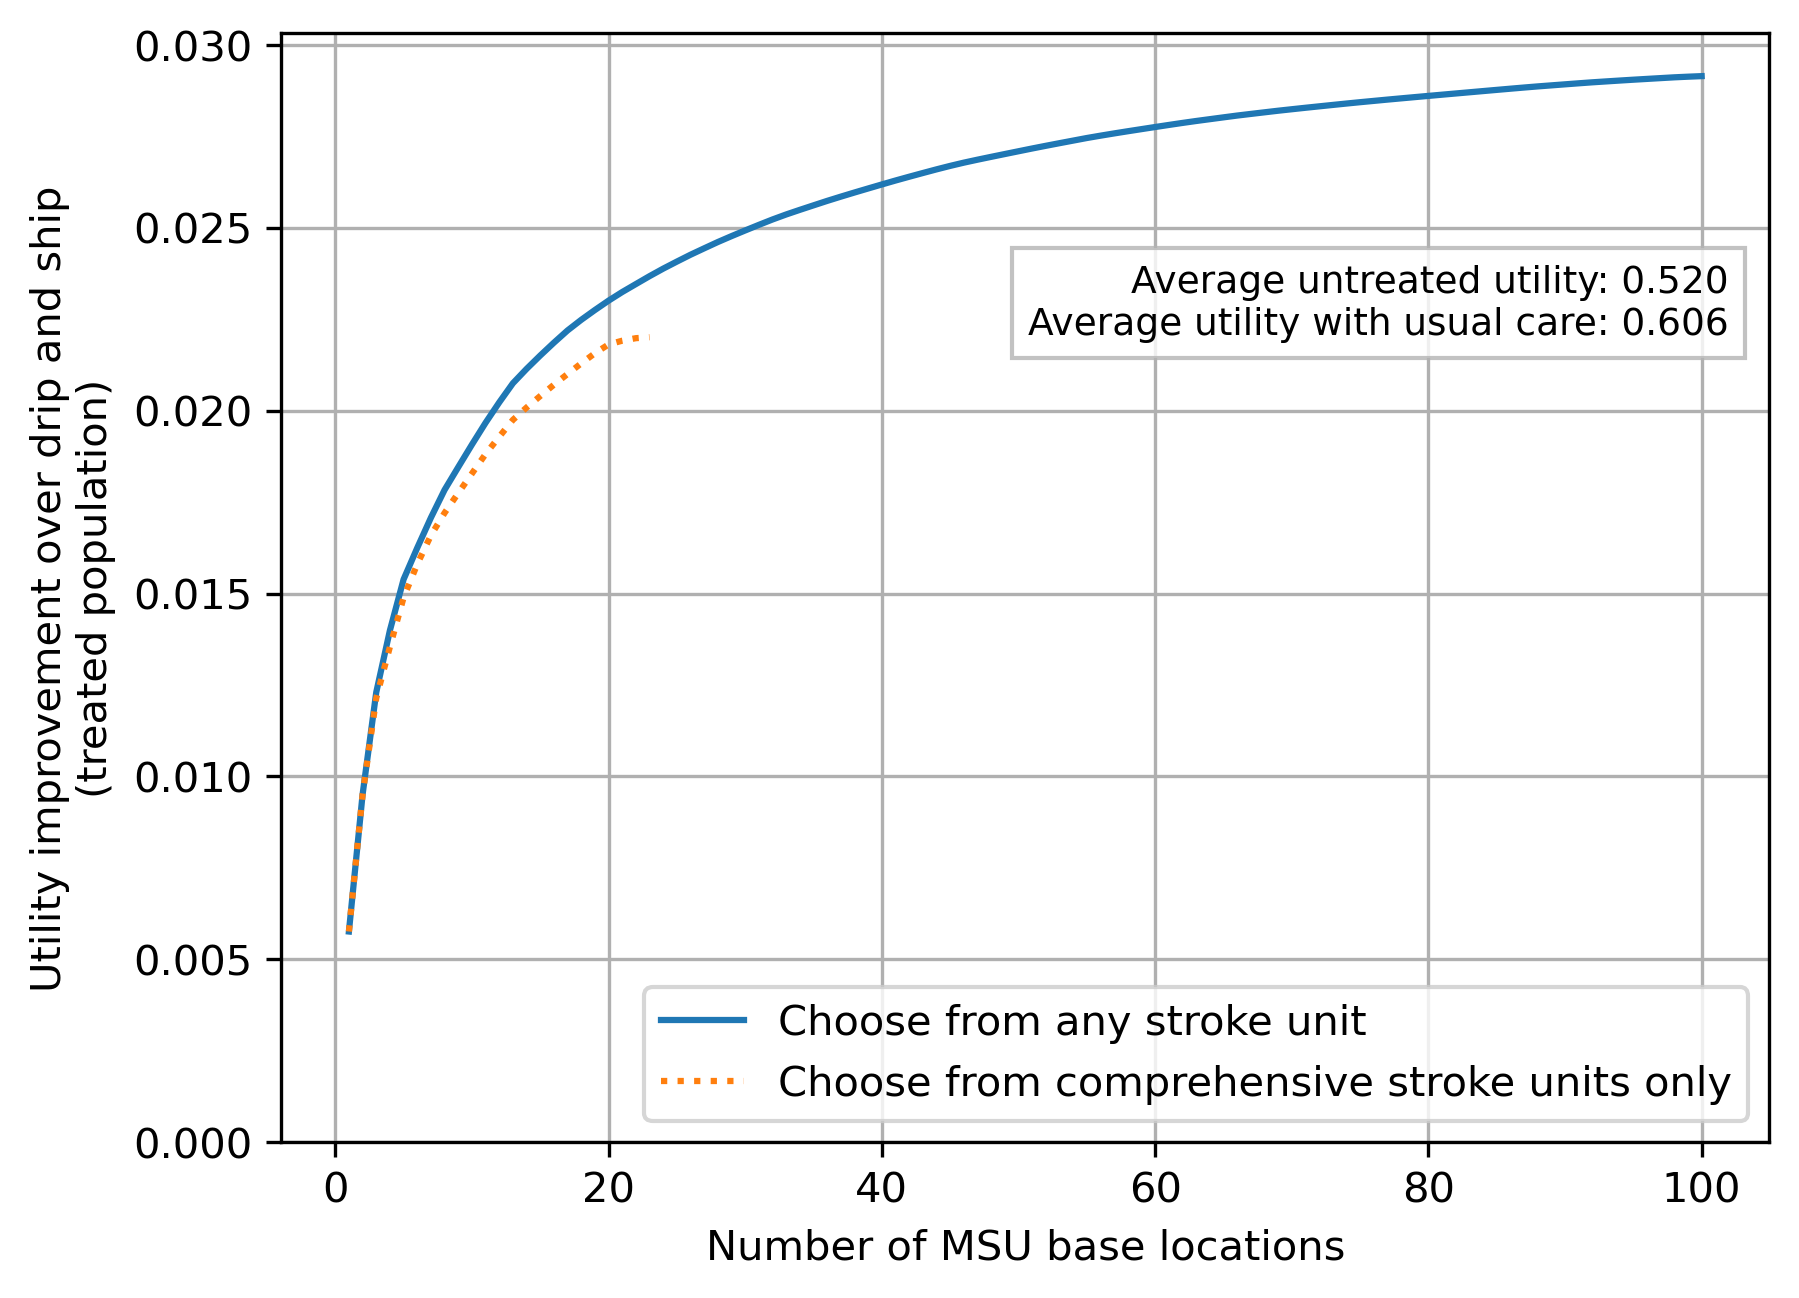
\includegraphics[width=0.5\linewidth]{images/msu_advantages_greedy.png}
    \caption{Increasing number of base locations of MSUs, with selection by a greedy algorithm based on improvements in utility. The utility improvement is for those patients treated by MSU rather than usual care. Units were choself either from any stroke unit type (solid line) or only from comprehensive stroke centres (dashed line).}
    \label{fig:greedy}
\end{figure}



\section{Discussion}

% Add something about OPTIMIST/SPPEDY

% Key findings

Overall we found a relatively marginal predicted benefit of MSUs across the whole country of England. Using likely process timing we found benefit was likely to be an increase of 0.015 to 0.03 in either utility or the proportion of patients with mRS 0-2 at 6 months. The benefit to nLVO was around 0.015 in either measure. The benefit to LVO was larger (around 0.035 in both measures), with the majority of this benefit coming from transferring LVOs directly to a MT-capable centre, avoiding the need for inter-hospital transfers and their associated delays. The benefit from earlier IVT is similar to that modeled by Holodinsky et al. \cite{holodinsky_jessalyn_k_what_2020}. Benefit was larger in the regions within reasonable travel distances of the MSU (similar catchments to those in the clinical trials). 

We found that the benefit of MSUs over usual care was critically dependent on rapid dispatch of the MSU and relatively rapid IVT ($\leq$30 minutes) on-scene. MSUs are therefore not an alternative to careful optimization of day-to-day operational activities.

The benefit of MSUs diminished with distance from the MSU base, though there was a halo effect for LVOs, with patients benefiting from direct transfer to MT-capable centres without excessive MSU arrival times. The diminishing benefit of MSUs is similar to that observed in clinical trials, where in Berlin the advantage of MSUs over usual care, when considering time to treatment, fell with distance from the MSU base \cite{koch_influence_2016}. MSUs centered in metropolitan areas are therefore not a solution to significantly improving stroke outcomes in more remote locations. If MSUs were based in remote locations there would be challenge of long MSU travel times if the MSU must maximise the number of patients seen each day. Additionally, MSUs will only partially solve the challenge of timely access to MT from remote areas. Maximising the net benefit of MSUs may therefore be at the cost of worsening equality of access to emergency stroke services, as when MSUs are placed in metropolitan areas they improve access to care for those that already have the best access.

We have modelled MSUs  being based at stroke centres. We compared basing MSUs at just comprehensive stroke centres (offering both IVT and MT) or at any type of stroke centres. The difference between these two approaches was marginal - likely because comprehensive stroke centres tend to be sited within large dense population centres, and so capture most population benefit of MSUs. It is possible to site MSUs in other locations, though most benefit will accrue from citing them in or near population centres, which is where stroke centres generally exist. As the number of base locations is increased the possible benefit increases, but with diminishing returns.

A possible difference between our model and real-world use of MSUs is that we assume that for patients within the time window of IVT and MT we assume a similar propensity of clinicians in MSUs and in usual care to give those treatments. This assumption allows us to isolate geographic effects. However, we know different stroke teams vary in their propensity to use IVT \cite{pearn_what_2023}. It is possible that MSUs will be staffed by clinicians more confident in using IVT, and so IVT use may increase not from the altered times to IVT, but by the patient being seen by clinicians more confident in using IVT. This could explain why Chen \textit{et al.} \cite{chen_systematic_2022} found such a significant (34\%) increase in use of IVT in MSU trials; it seems unlikely this change could come just from the speed improvements offered by MSUs.

We present results for patients seen by the MSU compared with usual care. A challenge will be identification of the correct patients to dispatch the MSU. In a 2024 review of Emergency Medical Services dispatcher recognition of stroke \cite{wenstrup_emergency_2024}, Wenstrup \textit{et al}. found sensitivity varied from 17.9\% to 83.0\%. Sensitivity median and interquartile range was 56\% (48\%-63\%). Positive predictive value was reported in 12 papers and ranged from 24.0\% to 87.7\%. Positive predictive values (PPV) median and interquartile range = 46\% (42\%-50\%). Typically therefore half of stroke patients are missed at ambulance dispatch, and only half of suspected stroke patients at dispatch are later confirmed to have a stroke. In one study it was found sensitivity for identifying stroke could be improved, but at the cost of positive predictive value; In a study on the effect of training call handlers \cite{watkins_training_2013}, on 464 patients, sensitivity improved from 63\% to 80\%, but PPV fell from 60.5\% to 39.0\%. Such uncertainty in the sensitivity and positive predictive value of identification of stroke patients makes it difficult to predict how many stroke patients will be seen by MSUs, as that number is limited by both sensitivity of dispatch (where stroke patients are missed) but also by positive predictive value which consumes MSU capacity, risking the MSU not being available as it attends a non-stroke patient. In addition to concerns around identifying patients for MSU dispatch, other implementation concerns have been raised in a qualitative study of clinician views of MSUs \cite{moseley_practitioner_2024}. This include concerns over how they would be staffed, where they would be based, and whether they will increase or reduce equity of access to emergency stroke care.

Our study adds to the evidence base on how MSUs may affect times to MT, especially when used more widely than areas close to comprehensive stroke centres. When the catchment area of MSUs extends out beyond the usual catchment area of comprehensive stroke centres, the MSU captures patients who would otherwise go to a local IVT-only stroke centre and require onward transfer for MT. MSUs therefore have significant potential to improve outcomes for those patients. This effect will be dependent on the MSU using CT-A to identify LVO patients.

\subsection{Study limitations}

Two key limitations have been discussed: Firstly, we isolated the geographic effects of MSUs and do not model how having an expert specialist team may increase IVT use simply by being more experienced, and so more confident, in use of IVT. Secondly, due to large uncertainties around sensitivity and positive predictive value of identification of stroke patients for MSU dispatch, we limit our study to modelling of outcomes of those who are seen by the MSU. Real-world benefit will be diluted by stroke patients being missed, or by MSU capacity not being available when required (especially if capacity is drained by low positive predictive value od suspected stroke). Similarly, for the same reason, we do not model how MSUs may affect emergency stroke admission numbers at hospitals (e.g. by changing effective catchment areas). It is possible that widespread use of MSUs could compromise the ability of some smaller hospitals to still provide IVT themselves (due to loss of experience). We also do not model other potential benefits of MSUs. In haemorrhagic stroke there may be potential to start reducing blood pressure sooner where that would benefit patients. In non-stroke patients it is possible that improved diagnosis by the MSU could help identify the best destination for that patient sooner, or may give more confidence in leaving the patient at home, saving hospital resources.

\subsection{Conclusions}

Overall we found a relatively small benefit from MSUs across the country, though some areas have greater benefit. It is possible that more selective targeting of MSUs use could help maximise benefit. A significant part of their potential benefit is derived from avoiding transfers for patients suitable for MT, reducing time to MT significantly. Maximising benefit from MSUs is critically dependent on rapid dispatch, and fast on-scene IVT. MSUs should not be seen as an alternative to optimizing day-to-day emergency stroke systems.
% References
\clearpage
\newpage
\printbibliography
\end{refsection}
\section{Declarations}

\subsection{Ethics approval and consent to participate}

No ethics/consent was required as no patients were recruited for this work, and no individual patient data was used.

\subsection{Consent for publication}

Not applicable.

\subsection{Availability of data and materials}

General model code is available at \url{https://github.com/stroke-modelling/muster2}.

Estimated travel times based on patient and hospital locations is available at \url{https://gitlab.com/michaelallen1966/1811_lsoa_to_acute_hospital_travel/}.

Code for estimation of stroke outcome depending on time to IVT or MT is available at \url{https://github.com/samuel-book/stroke_outcome/}, and is available as a Python package at \url{https://pypi.org/project/stroke-outcome/}.

\subsection*{Competing interests}

GF reports receiving consulting fees from AstraZeneca for management of stroke due to intracerebral haemorrhage (payment to his employer), Bayer for lecture on models of NHS industry working, CSL Behring for stroke trial consultancy, and being Chief Executive of Health Innovation Oxford and Thames Valley which has multiple joint working agreements and medical education grants with industry partners that are contracts with Oxford University Hospitals NHS Trust the host organisation for Health Innovation Oxford and Thames Valley.

\subsection{Authors' contributions}

All authors were involved in the design of the models, and in review/editing of the manuscript.

AL, MA, and KP, coded the models. AL and MA were the primary authors of the paper.


\subsection*{Funding}

This work was funded by National Institute for Health and Care Research (NIHR) Health Services and Delivery Research (Reference NIHR153982). MA was additionally funded by the NIHR Applied Research Collaboration South West Peninsula.

The views expressed in this publication are those of the authors and not necessarily those
of the NIHR or the Department of Health and Social Care.

\subsection*{Acknowledgments}

We thank all participants in co-production workshops which helped to inform the modelling described herein.

% Number for supplementary material
\newcommand{\beginsupplement}{
    \setcounter{section}{0}
    \renewcommand{\thesection}{S\arabic{section}}
    \setcounter{figure}{0}
    \renewcommand{\thefigure}{S\arabic{figure}}
    \setcounter{table}{0}
    \renewcommand{\thetable}{S\arabic{table}}

}
\begin{refsection} % Start referencing again for appendix
\beginsupplement
%TC:igno
\section{Supplementary material}


\begin{figure}
    \centering
    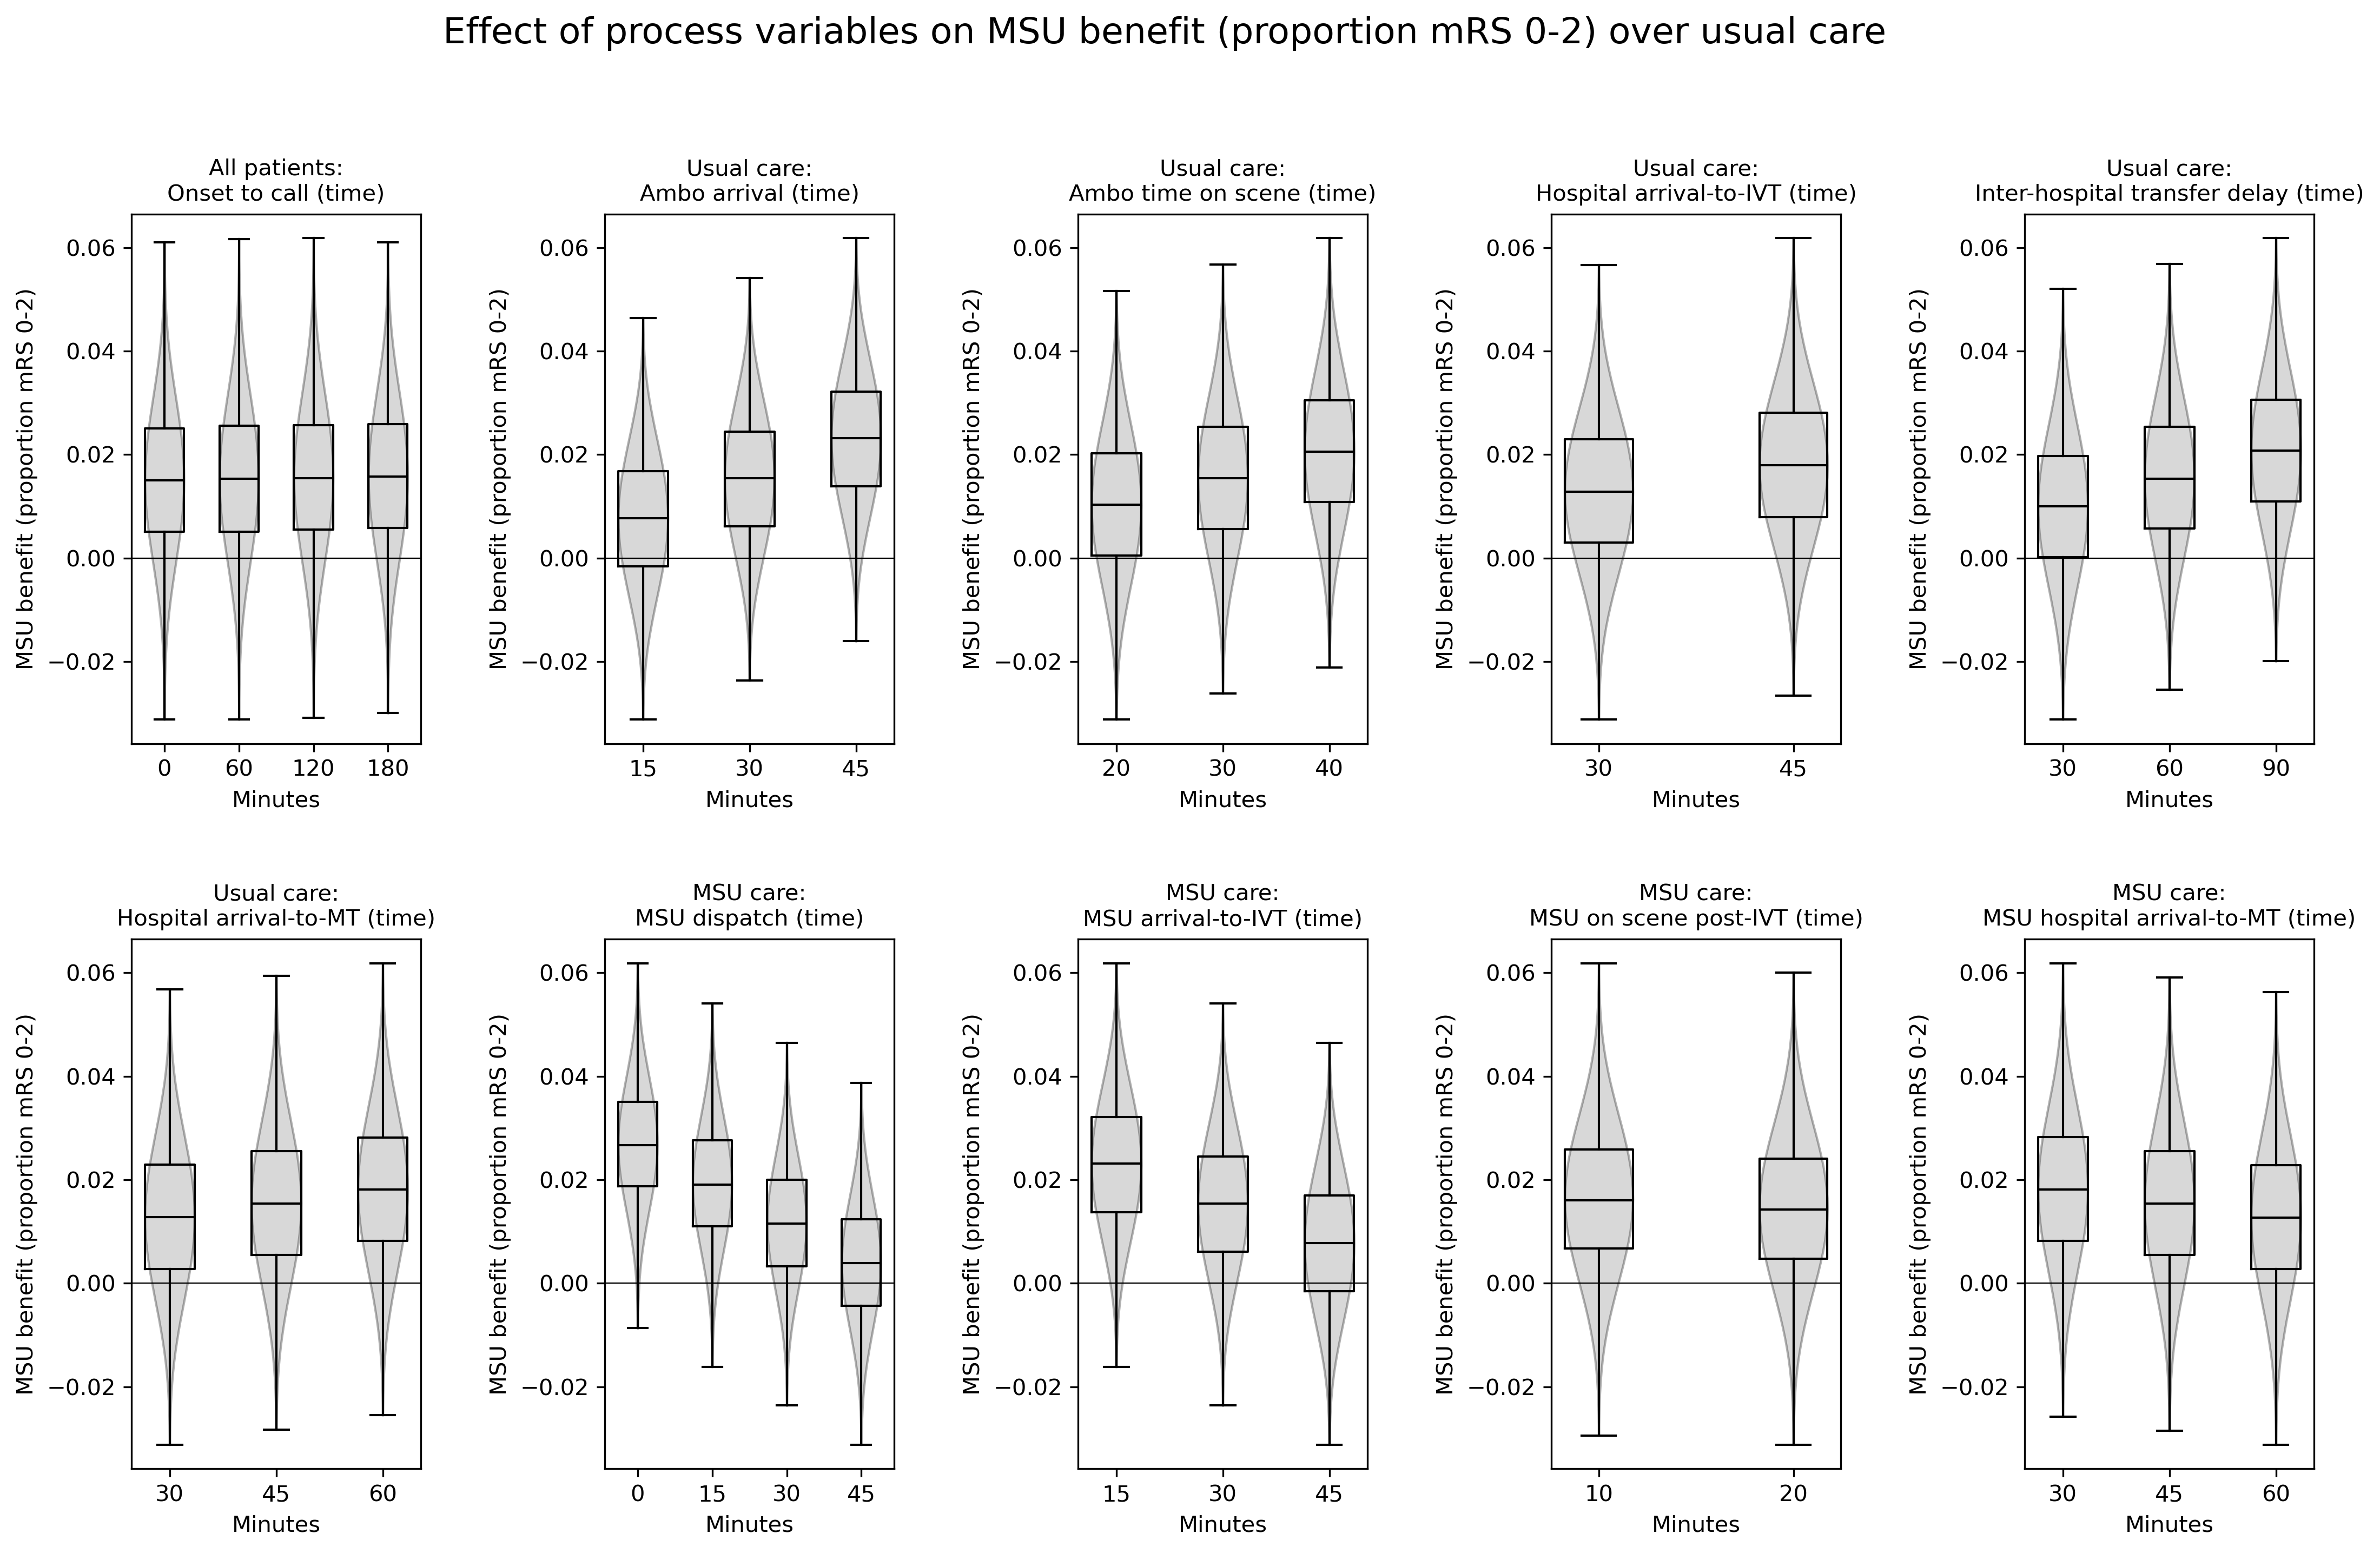
\includegraphics[width=1\linewidth]{images/msu_net_mrs_0-2_benefit.png}
    \caption{Enter Caption}
    \label{fig:enter-label}
\end{figure}

\begin{figure}
    \centering
    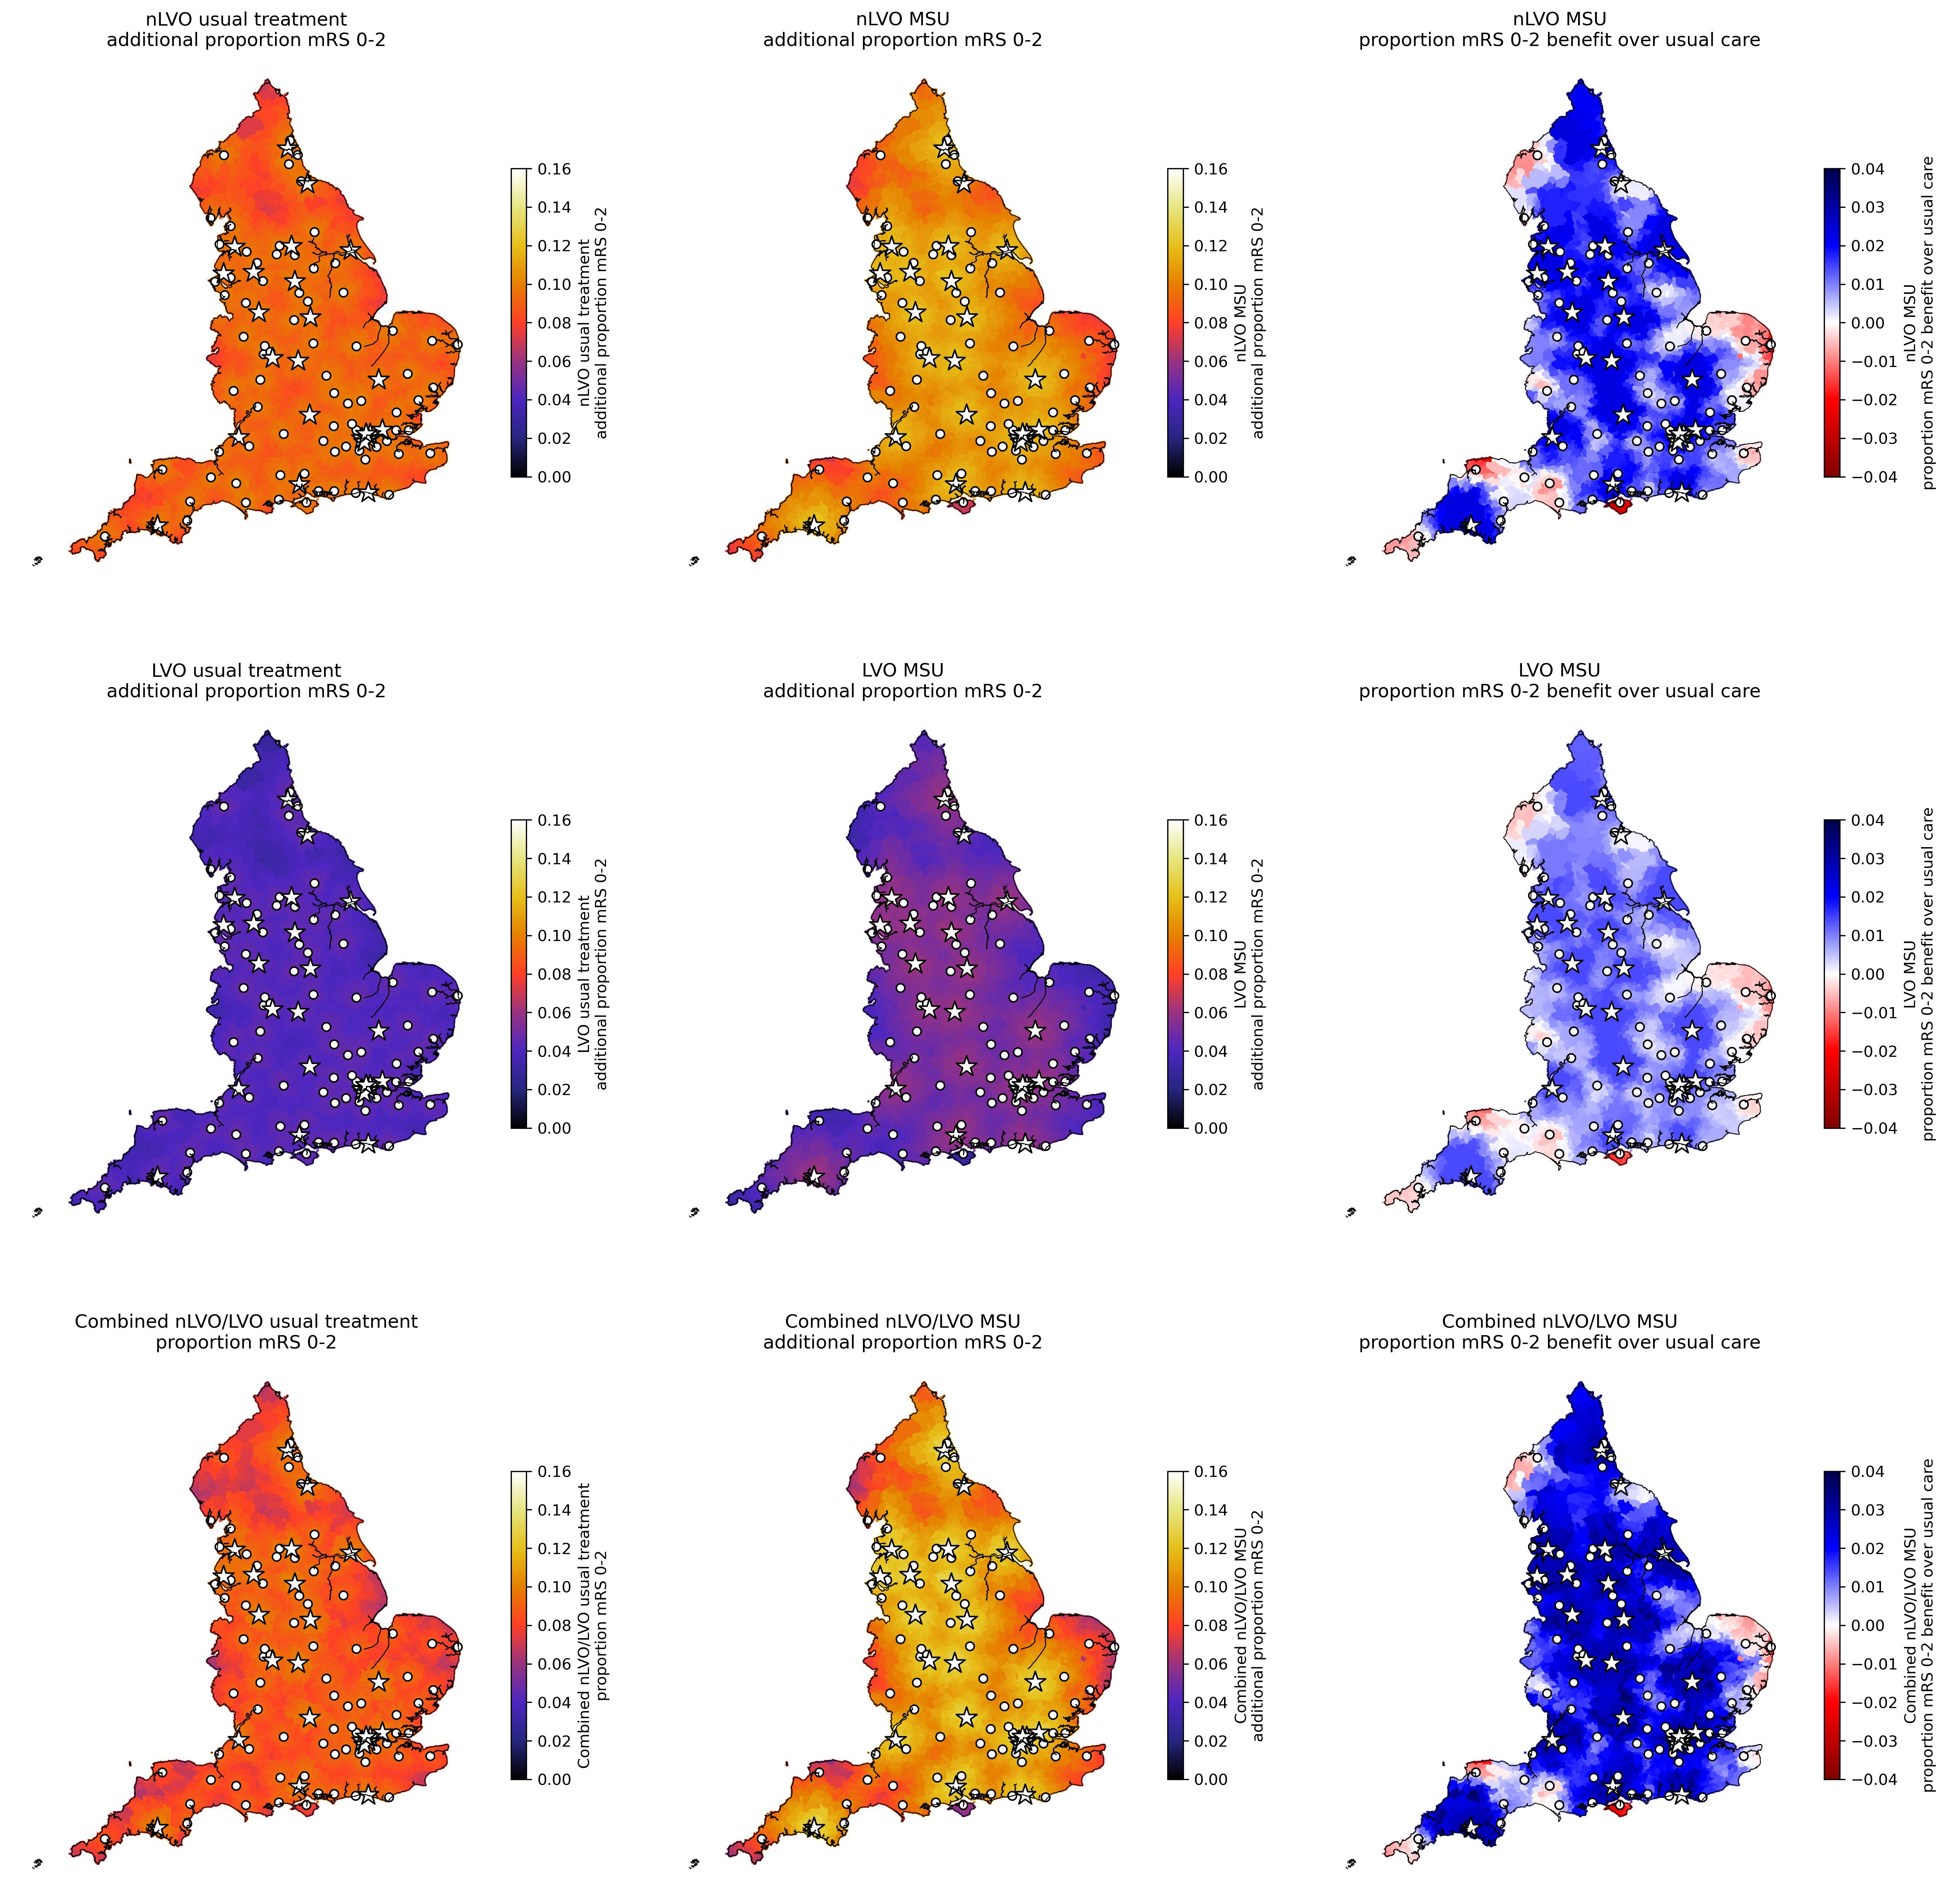
\includegraphics[width=1\linewidth]{images/map_mrs_0_2.jpg}
    \caption{Enter Caption}
    \label{fig:enter-label}
\end{figure}

%\section{Background research}

Mobile stroke units were first proposed in 2013 by Fassbender et al. \cite{fassbender_mobile_2003}. They were first trialed in Homberg, Germany (published 2015 \cite{walter_diagnosis_2012}), and first test in the US in Houston (published 2015, \cite{parker_establishing_2015}.

%%%%%%%%%%%%%%%%%%%%%%%%%%%%%%%%%%%%%%%%%% ECONOMIC BURDEN OF STROKE %%%%%%%%%%%%%%%%%%%%%%%%%%%%%%%%%%%%%%%%%%

\subsection{Economic burden of stroke}

%%%%%%%%%%%%%%%%%%%%%%%%%%%%%%%%%%%%%%%%%% AMBULANCE CALL OUT %%%%%%%%%%%%%%%%%%%%%%%%%%%%%%%%%%%%%%%%%%

\subsection{Ambulance call identification of stroke}

In a 2016 review of dispatch accuracy, Oostema et al \cite{oostema_dispatcher_2016} found "Regardless of the screening tool employed, dispatcher stroke recognition sensitivity was suboptimal (5 studies, range 41-83\%) as was the PPV (7 studies, range 42-68\%)" (see figure \ref{fig:oostema}.

\begin{figure}
    \centering
    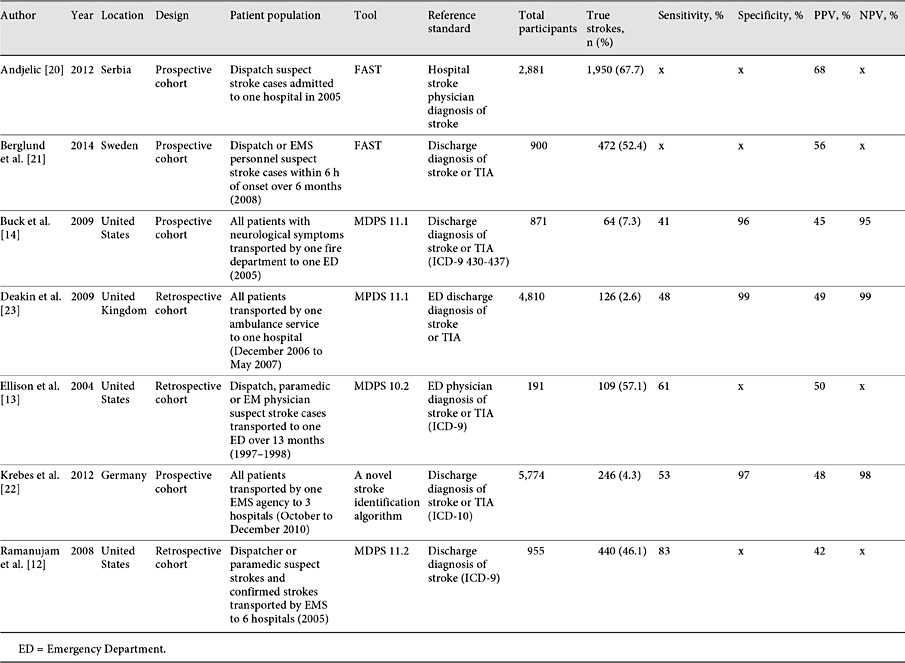
\includegraphics[width=0.9\linewidth]{images_background/oosetema_dispatch_accuracy}
    \caption{Oostema et al figure 2: Ambulance dispatch accuracy}
    \label{fig:oostema}
\end{figure}

In a 2024 review of Emergency Medical Services dispatcher recognition of stroke \cite{wenstrup_emergency_2024}, Wenstrup et al found sensitivity varied from 17.9\% to 83.0\% . Sensitivity median and interquartile range = 56\% (48\%-63\%). PPV was reported in 12 papers and ranged from 24.0\% to 87.7\%. PPV median and interquartile range = 46\% (42\%-50\%).

\begin{figure}
    \centering
    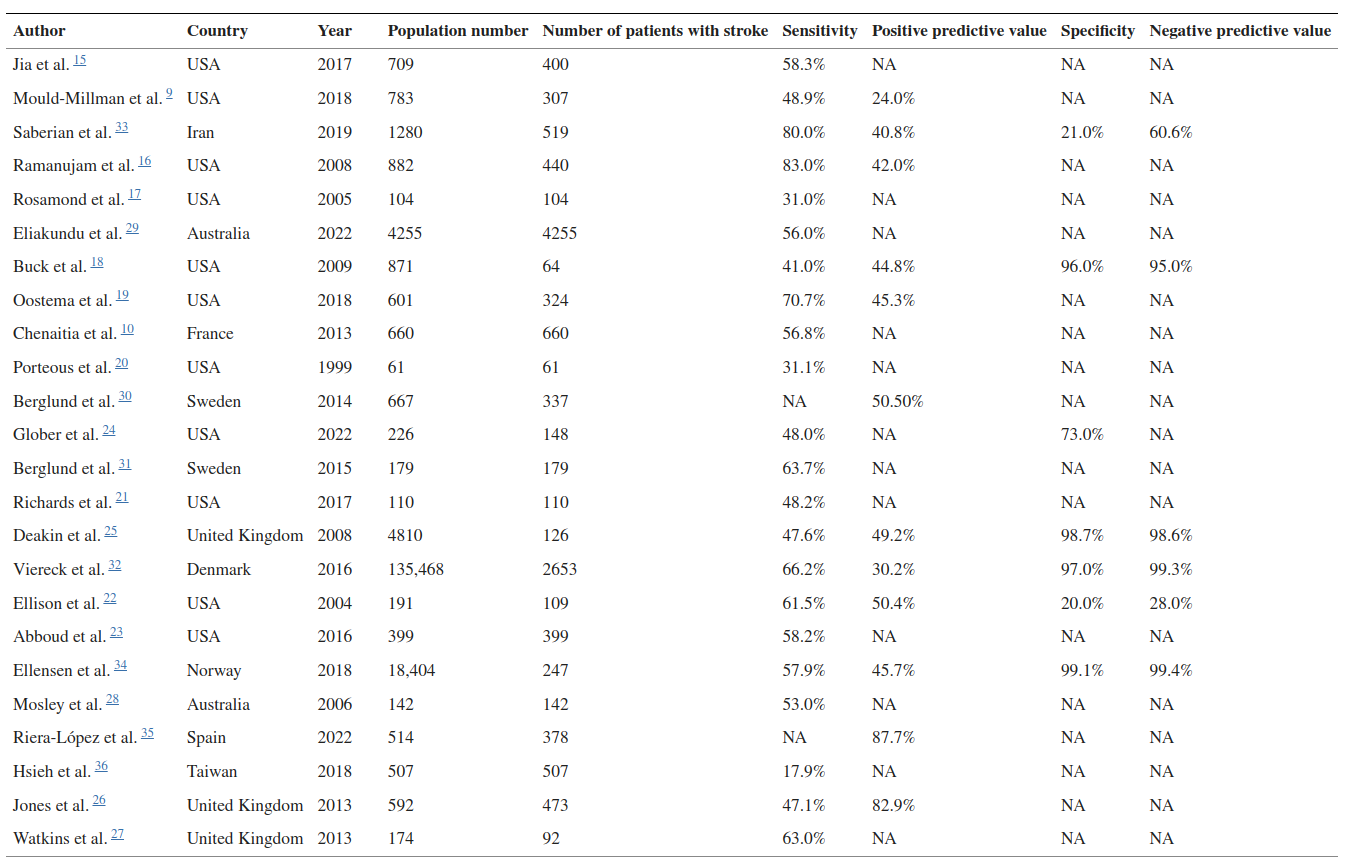
\includegraphics[width=0.75\linewidth]{images_background/wenstrup.png}
    \caption{Wenstrup et al table 1: Ambulance dispatch accuracy}
    \label{fig:wenstrup}
\end{figure}

\subsubsection{UK Studies}

North East Ambulance Service Study \cite{mcclelland_ambulance_2021}: In a study evaluating stroke identification by call handlers and clinicians in the North East Ambulance Service, 2,214 individual cases were analyzed. Call handlers identified acute stroke with a sensitivity of 51.5\% and a positive predictive value (PPV) of 12.8\%, while face-to-face clinicians had a sensitivity of 76.1\% and a PPV of 27.4\% The median on-scene time was 33 (IQR 25–43) minutes.

In a separate study on the North East Ambulance Service \cite{mcclelland_positive_2020} of 5,645 suspect stroke patients identified at call-out, 56\% were confirmed stroke, 6\% were TIA, and 38\% non-TIA stroke mimics.

In a study on the effect of training call handlers \cite{watkins_training_2013}, on 464 patients, sensitivity improved from 63\% to 80\%, but PPV fell from 60.5\% to 39.0\%. 

In a study in North West England \cite{jones_identification_2013} on 592 patients, sensitivity was 45\% and PPV 83\%.

\subsubsection{Stroke recognition systems}

Rudd et al reviewed hospital and pre-hospital stroke recognition system \cite{rudd_systematic_2016}; see figure \ref{fig:rudd}.

\begin{figure}
    \centering
    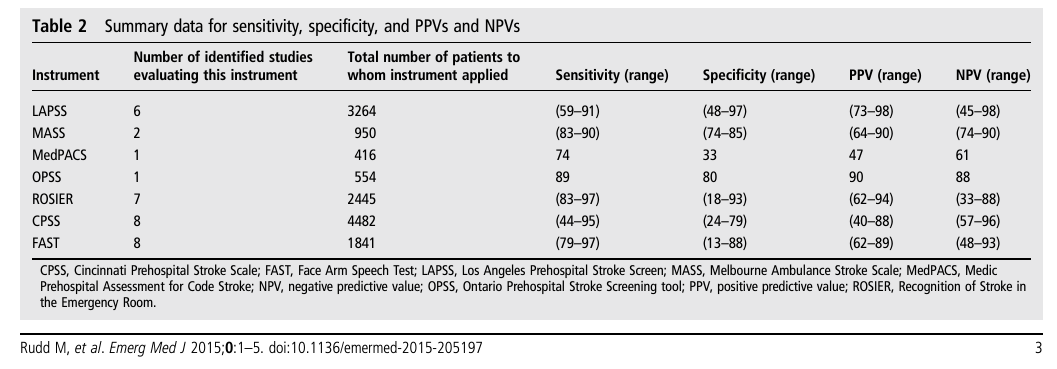
\includegraphics[width=0.9\linewidth]{images_background/rudd.png}
    \caption{Stroke recognition system, from Rudd et al}
    \label{fig:rudd}
\end{figure}

ROSIER (Recognition of Stroke in the Emergency Room):

\begin{itemize}
    \item Facial weakness
    \item Arm weakness
    \item Leg weakness
    \item Speech disturbance
    \item Visual field defects
\end{itemize}



%%%%%%%%%%%%%%%%%%%%%%%%%%%%%%%%%%%%%%%%%% FATIMA METANALYSIS %%%%%%%%%%%%%%%%%%%%%%%%%%%%%%%%%%%%%%%%%%

\subsection{Fatima review and metanalysis on mobile stroke units 2022 \cite{fatima_mobile_2020}
}

A total of 21,297 patients from 11 publications (seven randomized controlled trials and four non-randomized controlled trials including prospective cohort studies) were retrieved. This included 6065 (28.4\%) of the patients treated in the mobile stroke unit and 71.6\% (15,232) of the patients managed in the conventional care.

The mean age at clinical presentation (70.1 vs. 71.05) and National Institute Health Stroke Scale (9.8 vs. 8.4) was comparable (p>0.05) in patients treated with mobile stroke unit and conventional care, respectively.

The mean time-to-treatment window was significantly shorter among the patients treated in mobile stroke unit compared to conventional care (62min vs. 75min; p=0.03, respectively).

The pooled analysis of clinical outcome at day 7 indicated that patients treated in mobile stroke unit had 1.46-folds higher likelihood of better clinical outcome (modified Rankin scale 0–2) than those in the hospital (odds ratio: 1.46, 95\% confidence interval: 1.306–2.03, p=0.02).

However, there was no significant difference in terms of mortality (odds ratio: 0.98, 95\% confidence interval: 0.81–1.18, p=0.80), stroke-related neurological deficits (odds ratio: 1.37, 95\% confidence interval: 0.81–2.32, p=0.24), and other serious adverse events (odds ratio: 0.69, 95\% confidence interval: 0.39–1.20, p=0.19) among patients treated in mobile stroke unit versus conventional care (figure \ref{fig:background_fatima_fig_5}).

\begin{figure}
    \centering
    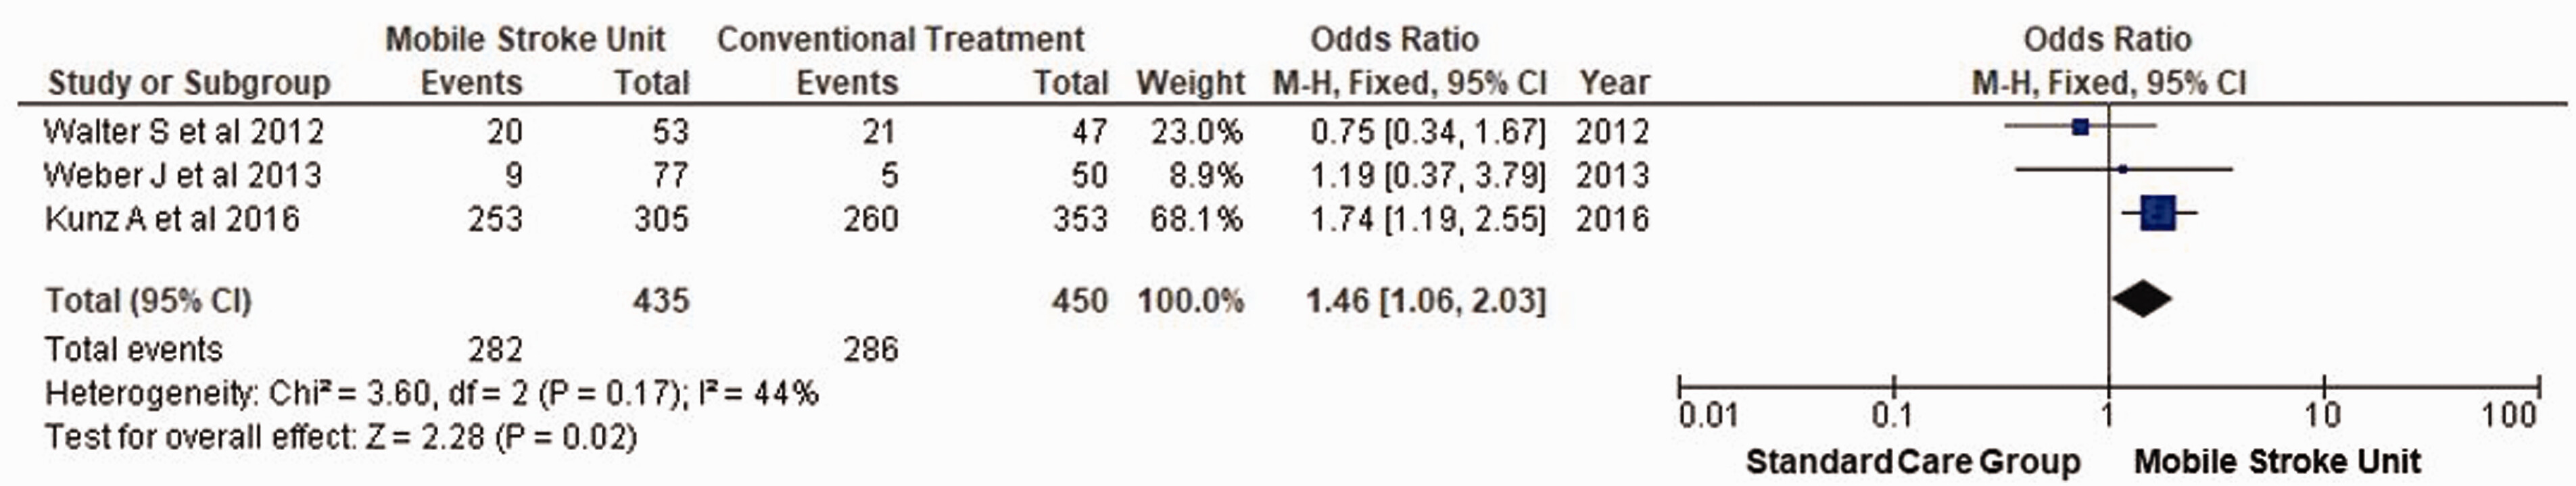
\includegraphics[width=0.5\linewidth]{images_background/fatima_fig_5}
    \caption{Pooled analysis of mRS at 907days (Fatima et al., 2020)}
    \label{fig:background_fatima_fig_5}
\end{figure}

%%%%%%%%%%%%%%%%%%%%%%%%%%%%%%%%%%%%%%%%%% CHEN META-ANLYSIS %%%%%%%%%%%%%%%%%%%%%%%%%%%%%%%%%%%%%%%%%%

\subsection{Chen review and metanalysis on mobile stroke units 2022 \cite{chen_systematic_2022}}

A total of 22,766 patients from 16 publications were included. In total 7,682 (n = 33.8\%) were treated in the MSU and 15,084 (n = 66.2\%) in the conventional EMS.

Economic analysis were available in four studies, of which two were based on trial data and the others on model simulations. The pooled analysis of time metrics indicated a mean reduction of 33 min and 28 minutes in the time-to-therapy and time-to-CT completion, respectively in the MSU.

There was no significant difference on stroke-related neurological events and in-hospital mortality between the MSU and EMS.

The proportion of patients with modified Ranking scale (mRS) of 0–2 at 90 days from onset was higher in the MSU than EMS (p < 0.05, figure \ref{fig:background_chen_fig_5}). The proportion receiving thrombolysis was 27.7\% in EMS and 37.3\% in MSU. Of those receiving thrombolysis, the proportion mRS0-2 was 59.3\% using EMS and 66.2\% using MSU. In all patients, the proportion mRS0-2 was 58.8\% using EMS and 64.5\% using MSU.

\begin{figure}
    \centering
    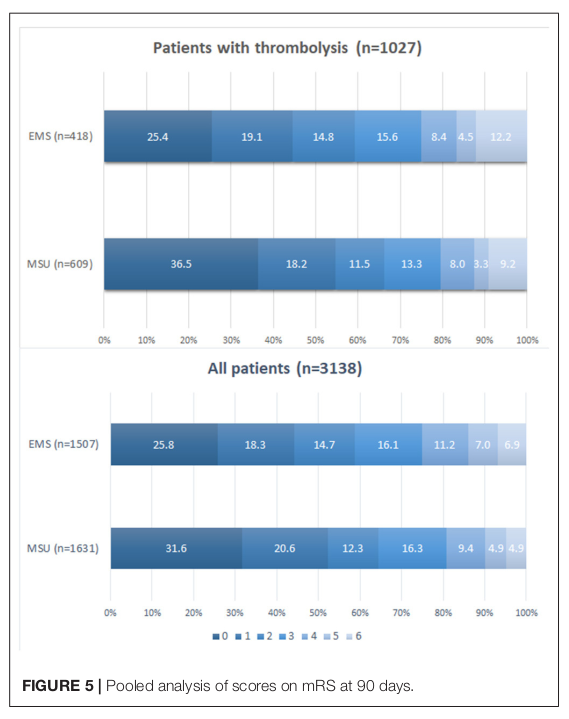
\includegraphics[width=0.5\linewidth]{images_background/chen_fig_5}
    \caption{Pooled analysis of mRS at 90 days (Chen et al., 2021)}
    \label{fig:background_chen_fig_5}
\end{figure}

MSU displayed favorable benefit-cost ratios and incremental cost-effectiveness ratio (\$31,911 /QALY and \$38,731 per DALY) comparing to EMS in multiple economic publications.

%%%%%%%%%%%%%%%%%%%%%%%%%%%%%%%%%%%%%%%%%% INDIVIDUAL TRIALS %%%%%%%%%%%%%%%%%%%%%%%%%%%%%%%%%%%%%%%%%%

\subsection{Individual trials - Germany}

\subsubsection{Walter et al, RCT, 2012, Homberg, Germany \cite{walter_diagnosis_2012}}

MSU described in an earlier paper \cite{walter_bringing_2010}.

\begin{figure}[ht]
    \centering
    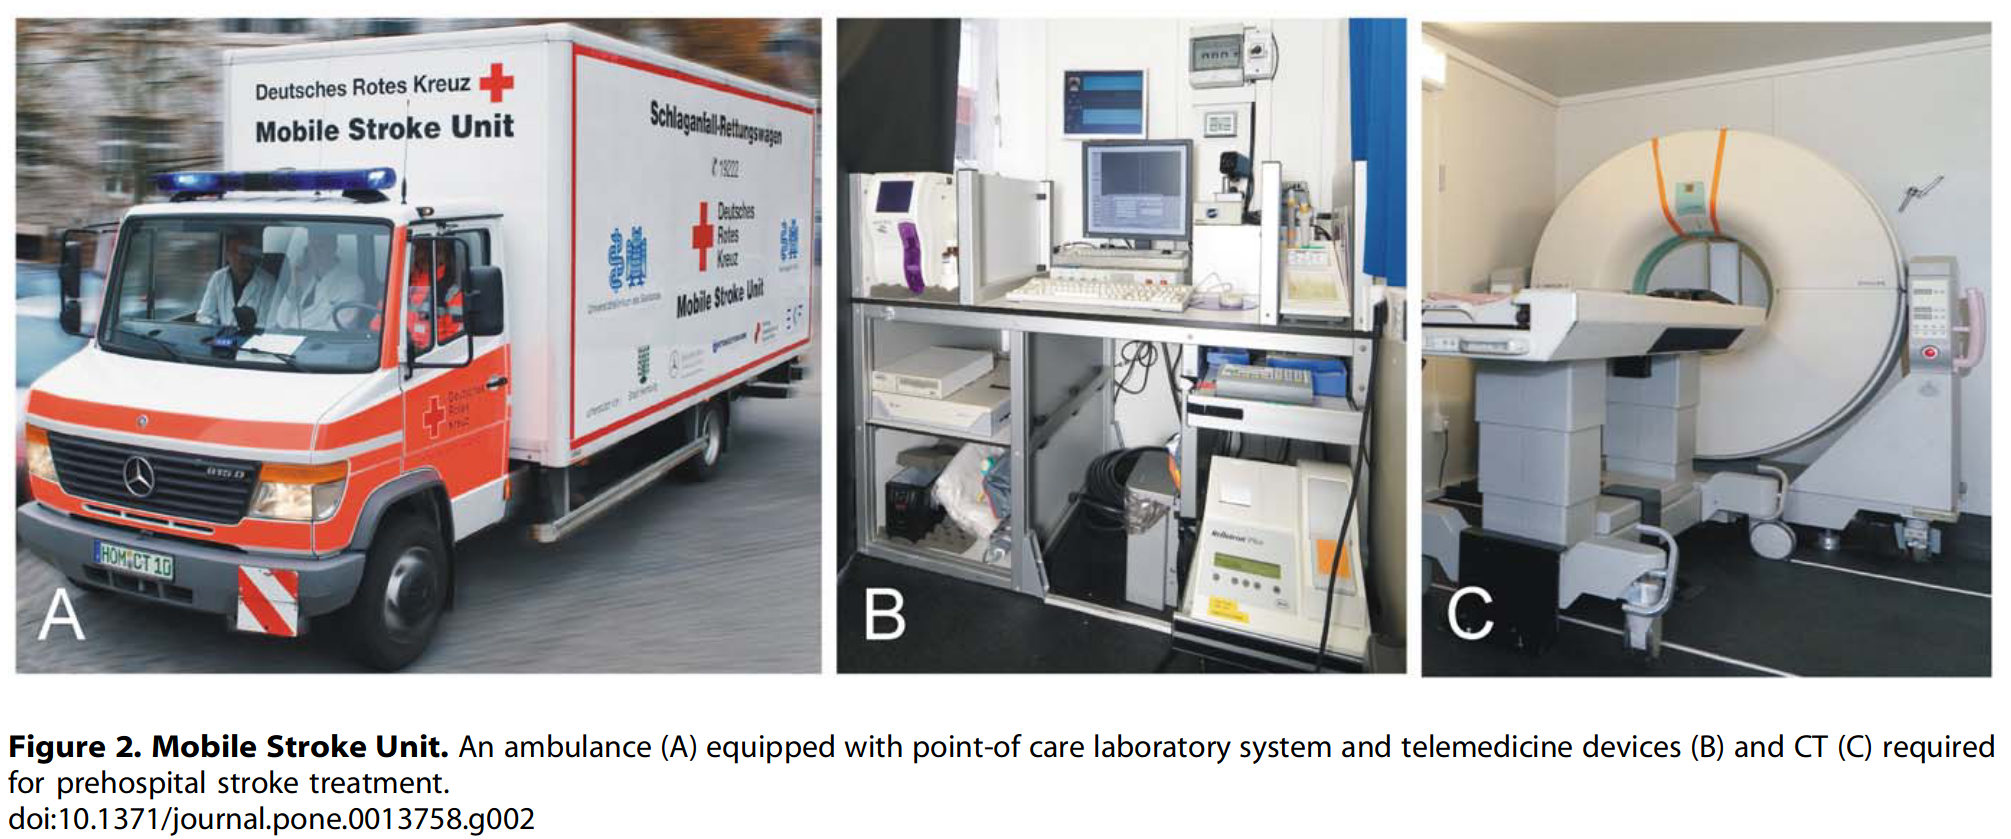
\includegraphics[width=0.95\linewidth]{images_background/walter_msu}
    \caption{The Mobile Stroke Unit, as used by Walter et al.}
    \label{fig:walter_msu}
\end{figure}

Study basics:

\begin{markdown}
* First controlled trial on MSU
* 100 patients (53 MSU, 47 normal care)
* Homberg, Germany (30km radius)
* Dispatch is one symptom of ROSIER: 55\% had confirmed ischaemic stroke, 17\% TIA, 11\% haemorrhage.
* 3 hour onset-to-thrombolysis was used as thrombolysis cut-off
* The MSU team included a paramedic, a stroke physician, and a neuroradiologist
* Primary outcome: therapy decision
\end{markdown}

Results (MSU vs. normal care, with IQR):

\begin{markdown}
* Thrombolysis rate: 23\% vs. 17\% (33\% increased based on un-rounded values)
* Call-to-thrombolysis (min): 38 (34-42) vs. 73 (60-93)
* Symptom onset to therapy decision (min): 56 (43–103) vs. 104 (80–156)
* Call to end of CT (min): 34 (30–38) vs. 71 (62–87)
\end{markdown}

There was no information on call-to-ambulance/MSU arrival times, and MSU or hospital arrival-to-treatment times. But discussion says that at that time arrival-to-thrombolysis target was 60 min, with lots of patients breaching that time. The authors note that MSU strategy provides an opportunity for  blood-pressure management well before hospital arrival.

\subsubsection{Ebinger et al., Berlin, 2014 Timing trial \cite{ebinger_effect_2014}}

\begin{markdown}
* Berlin, Germany
* 6182 adult patients. MSU available in certain weeks
* Thrombolysis rates in ischemic stroke were 29\% (310/1070) during MSU weeks and 33\% (200/614) after MSU deployment vs 21\% (220/1041) during control weeks
* Compared with thrombolysis during control weeks, there was a reduction of 15 minutes in alarm-to-treatment times in the catchment area during STEMO weeks (76.3 min vs 61.4 min P < .001).
* Among patients for whom STEMO was deployed, mean alarm-to-treatment time (51.8 min) was shorter by 25 minutes than during control weeks.
* MSU deployment incurred no increased risk for intracerebral hemorrhage 
\end{markdown}

\subsubsection{Wendt et al., RCT, Berlin \cite{wendt_improved_2015}}

Focus is on delivering patients to the right hospital:

\begin{markdown}
* Berlin
* Normal care and MSU care week
* 1804 of 6182 (29\%) patients received MSU care and 4378 of 6182 (71\%) patients conventional care.
* 245 of 2110 (11.6\%) patients with cerebrovascular events were sent to hospitals without Stroke Unit in conventional care when compared with 48 of 866 (5.5\%; P<0.01) patients in MSU care.
* The delivery rate of patients with intracranial hemorrhage to hospitals without neurosurgery department was 43.0\% (65 of 151) in conventional care and 11.3\% (7 of 62) in MSU care (P<0.01).
* 89\% sensitivity, and 77\% specificity for pre-hospital diagnosis of stroke/TIA (79\% PPV, 87\% NPV)
\end{markdown}

\subsubsection{Ebinger et al., RCT, Berlin, 2015 \cite{ebinger_effects_2015}}

* The MSU was staffed with a neurologist trained in emergency medicine, a
paramedic, and a radiology technician. A neuroradiologist was on call to evaluate images acquired on board the STEMO via a teleradiology connection.
* Thrombolysis rates in ischemic stroke were 200 of 614 patients (32.6\%) when MSU was deployed and 330 of 1497 patients (22.0\%) when conventional care was administered (P < .001).
* Among all patients who received thrombolysis, the proportion of golden hour thrombolysis was 6-fold higher after MSU deployment (62 of 200 patients [31.0\%] vs 16 of 330 [4.9\%]; P < .01).
* Compared with patients with a longer time from symptom onset to treatment, patients who received golden hour thrombolysis had no higher risks for 7- or 90-day mortality (adjusted odds ratios, 0.38 [95\% CI, 0.09-1.70]; P = .21 and 0.69 [95\% CI, 0.32-1.53]; P = .36) and were more likely to be discharged home (adjusted odds ratio, 1.93 [95\% CI, 1.09-3.41]; P = .02).
* No detailed comparison or breakdown of times was given.

\subsubsection{Travel times in Berlin \cite{koch_influence_2016}}

With increasing distance from MSU base:

* Time from call to hospital arrival increases in comparison with normal care
* Catchment population increases in proportion to square of radius
* Call to treatment increases, but was better than normal care in all zones, but advantage dropped from 35 mins (zone 1) to 18 minutes (zone 4)

* MSU 8-18 minutes call-to-arrival, 25 mins from arrival to completion of imaging (35-50 min call to imaging), and 35-40 mins arrival to treatment (40-60 min call-to-treatment).
* Normal care about 7 min call to ambo arrival, 35 min call to hospital arrival, 40-45 min door-t-needle, 75-80 min call-treatment


\begin{figure}
    \centering
    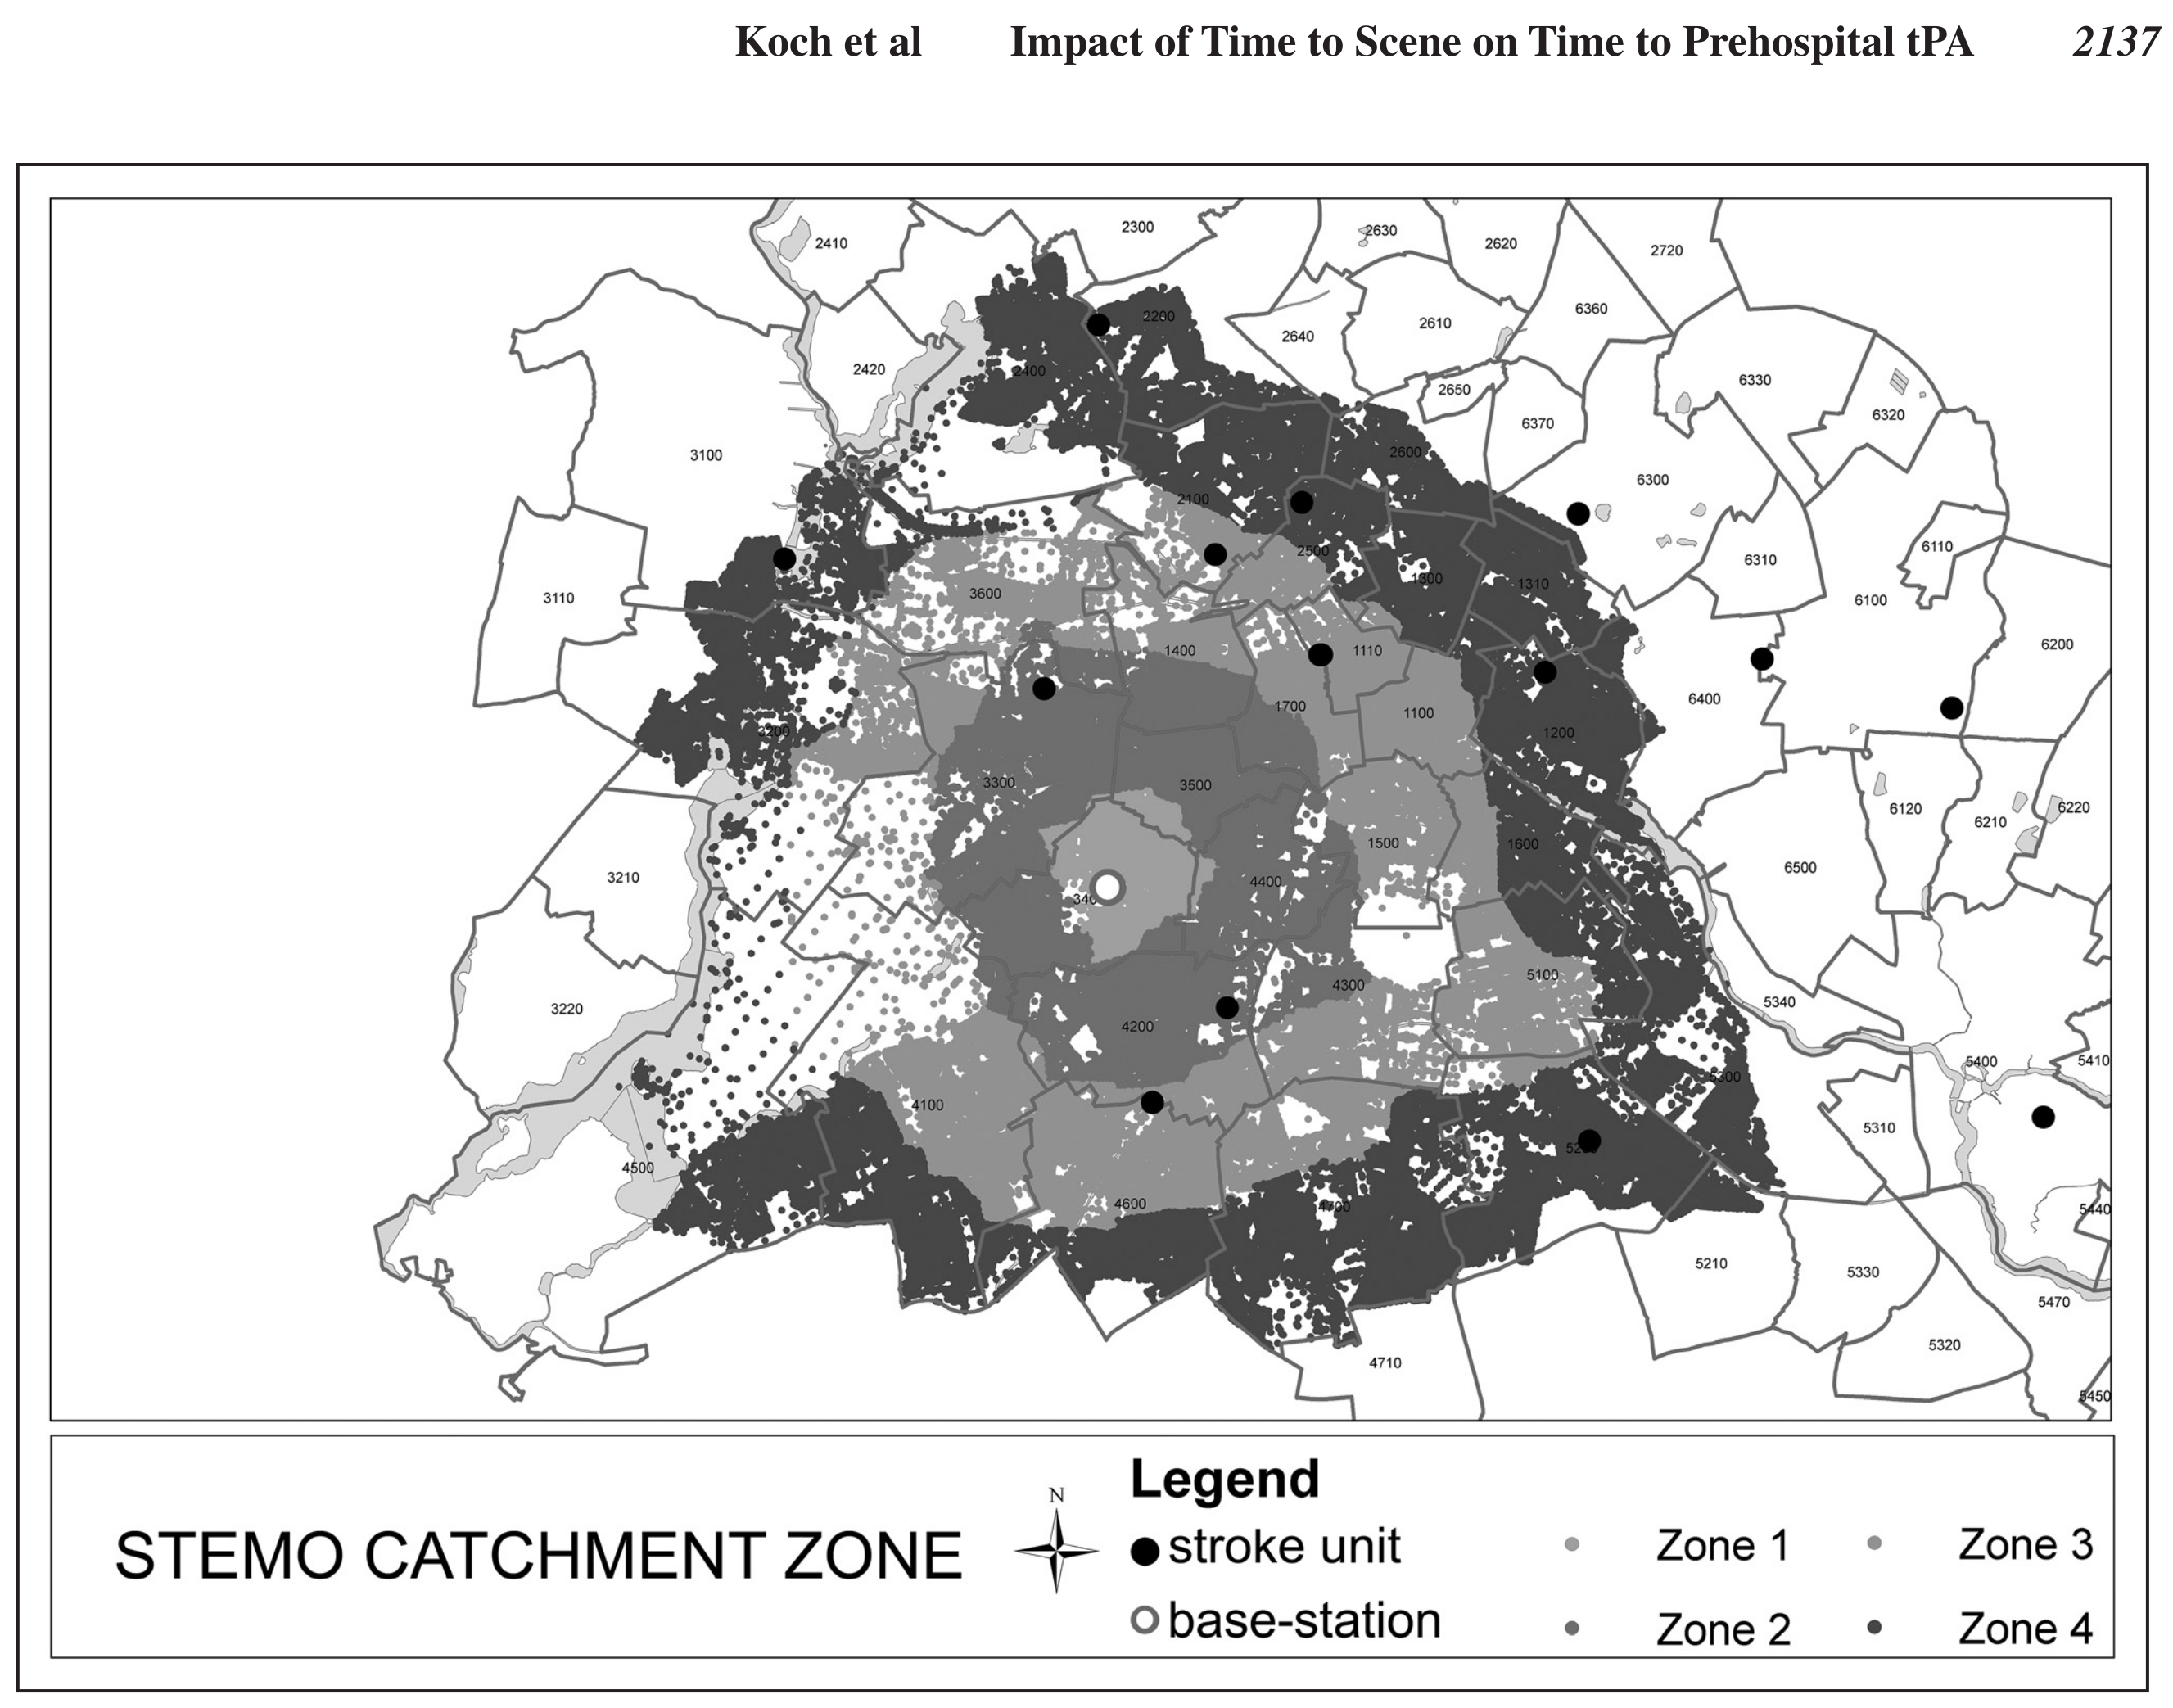
\includegraphics[width=0.9\linewidth]{images_background/berlin_map_2.png}
    \caption{Map of Berlin MSU study area }
    \label{fig:map_berlin_2}
\end{figure}

\begin{figure}
    \centering
    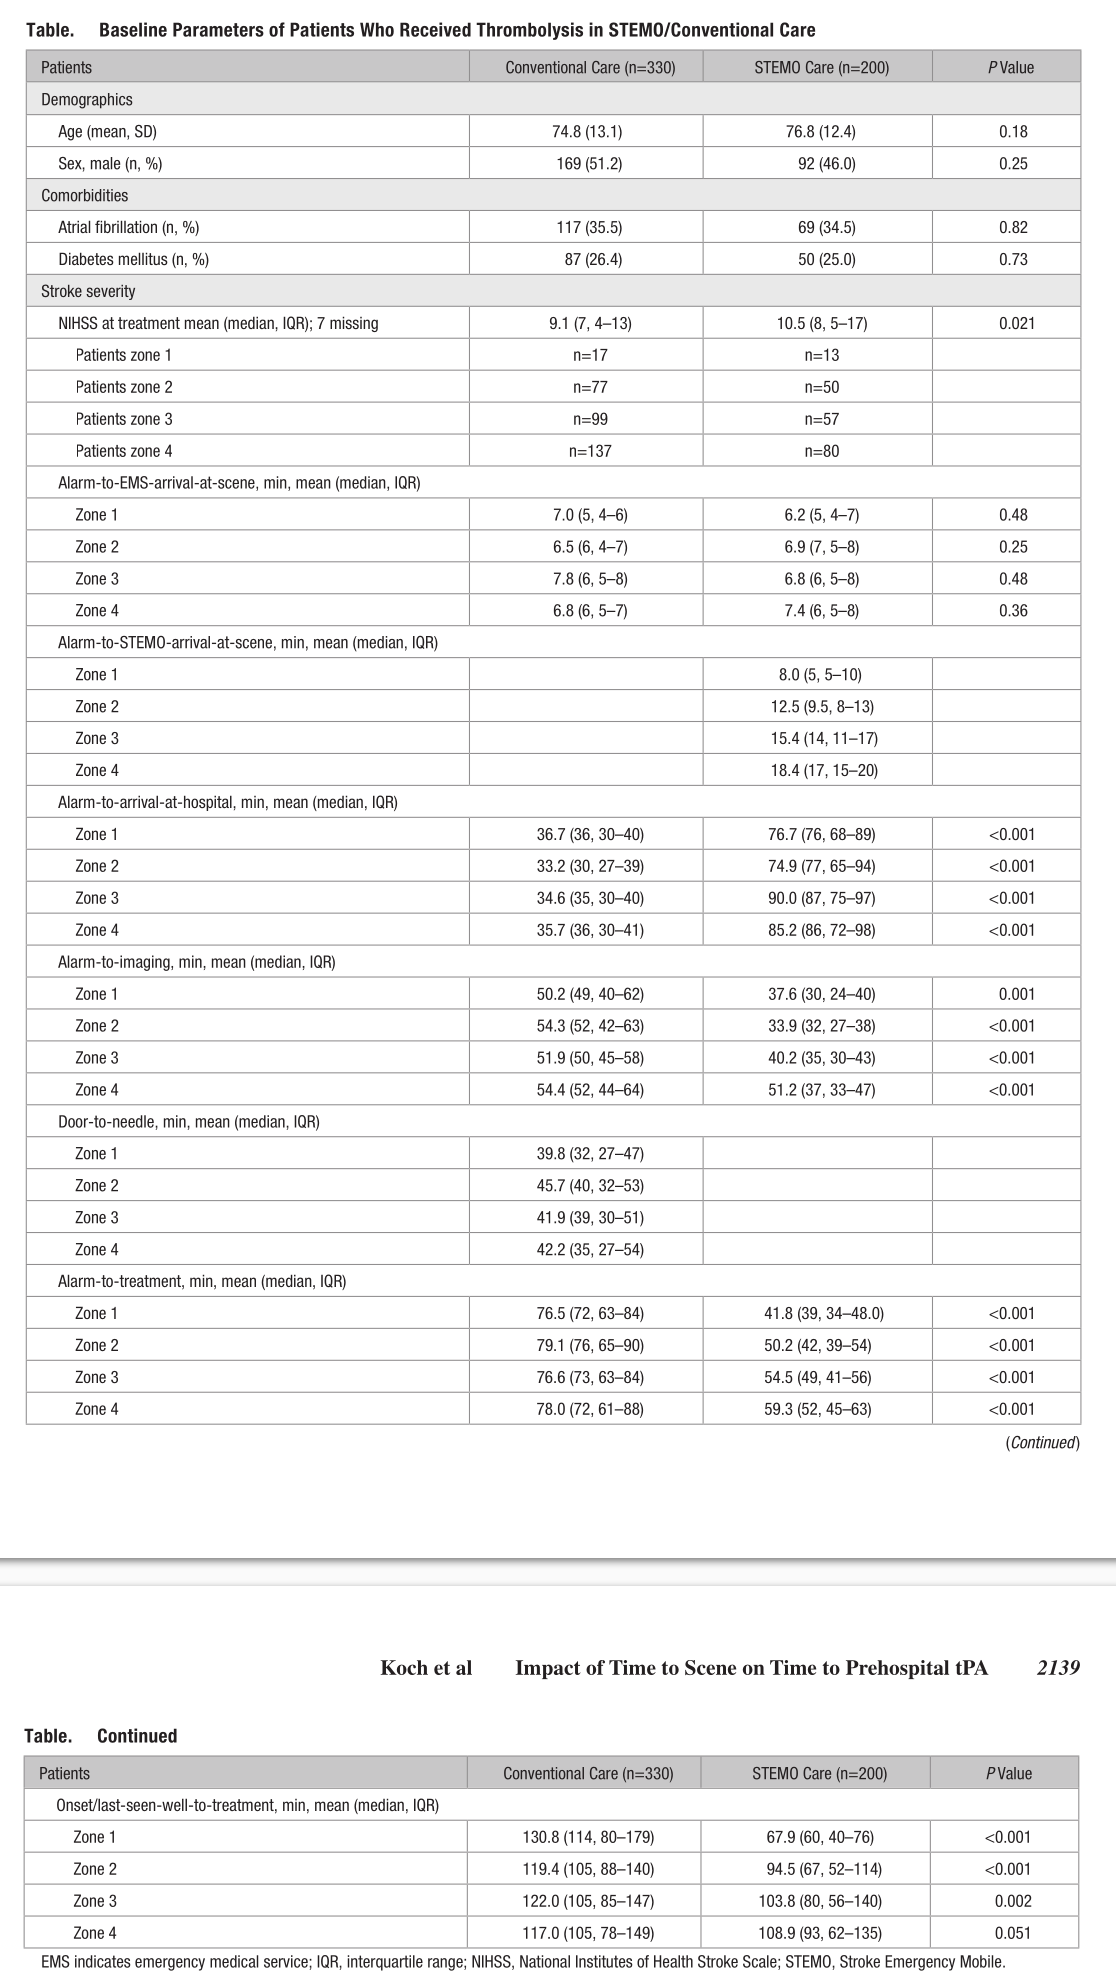
\includegraphics[width=0.5\linewidth]{images_background/koch_timings.png}
    \caption{Timing from Berlin study; from Koch et al.}
    \label{fig:kock_timings}
\end{figure}

\subsubsection{Kunz et al., Berlin, Observational study \cite{kunz_functional_2016}}

* Logistic regression analysis
* The primary outcome was the proportion of patients who had lived at home without assistance before stroke and had a 3-month modified Rankin Scale mRS) score of 1 or lower.
* Findings:  Between Feb 5, 2011, and March 5, 2015, 427 patients were treated within the MSU vehicle and their data were entered into a pre-hospital registry. 505 patients received conventional care and their data were entered into an in-hospital thrombolysis registry. Of these, 305 patients in the MSU group and 353 in the conventional care group met inclusion criteria and were included in the analysis. 161 (53\%) patients in the MSU group versus 166 (47\%) in the conventional care group had an mRS score of 1 or lower (p=0·14). Compared with conventional care, adjusted odds ratios (ORs) for MSU care for the primary outcome (OR 1·40, 95\% CI 1·00–1·97; p=0·052) were not significant. Intracranial haemorrhage (p=0·27) and 7-day mortality (p=0·23) did not differ significantly between treatment groups.
* Interpretation We found no significant difference between the proportion of patients with a mRS score of 1 or lower receiving MSU care compared with conventional care. However, our results suggest that pre-hospital start of intravenous thrombolysis might lead to improved functional outcome in patients. This evidence requires substantiation in future large-scale trials.

Comparison was MSU or normal ambulances and in-hospital care at the Charité Campus Benjamin Franklin in Berlin (see fig \ref{map_berlin_1}).

\begin{figure}
    \centering
    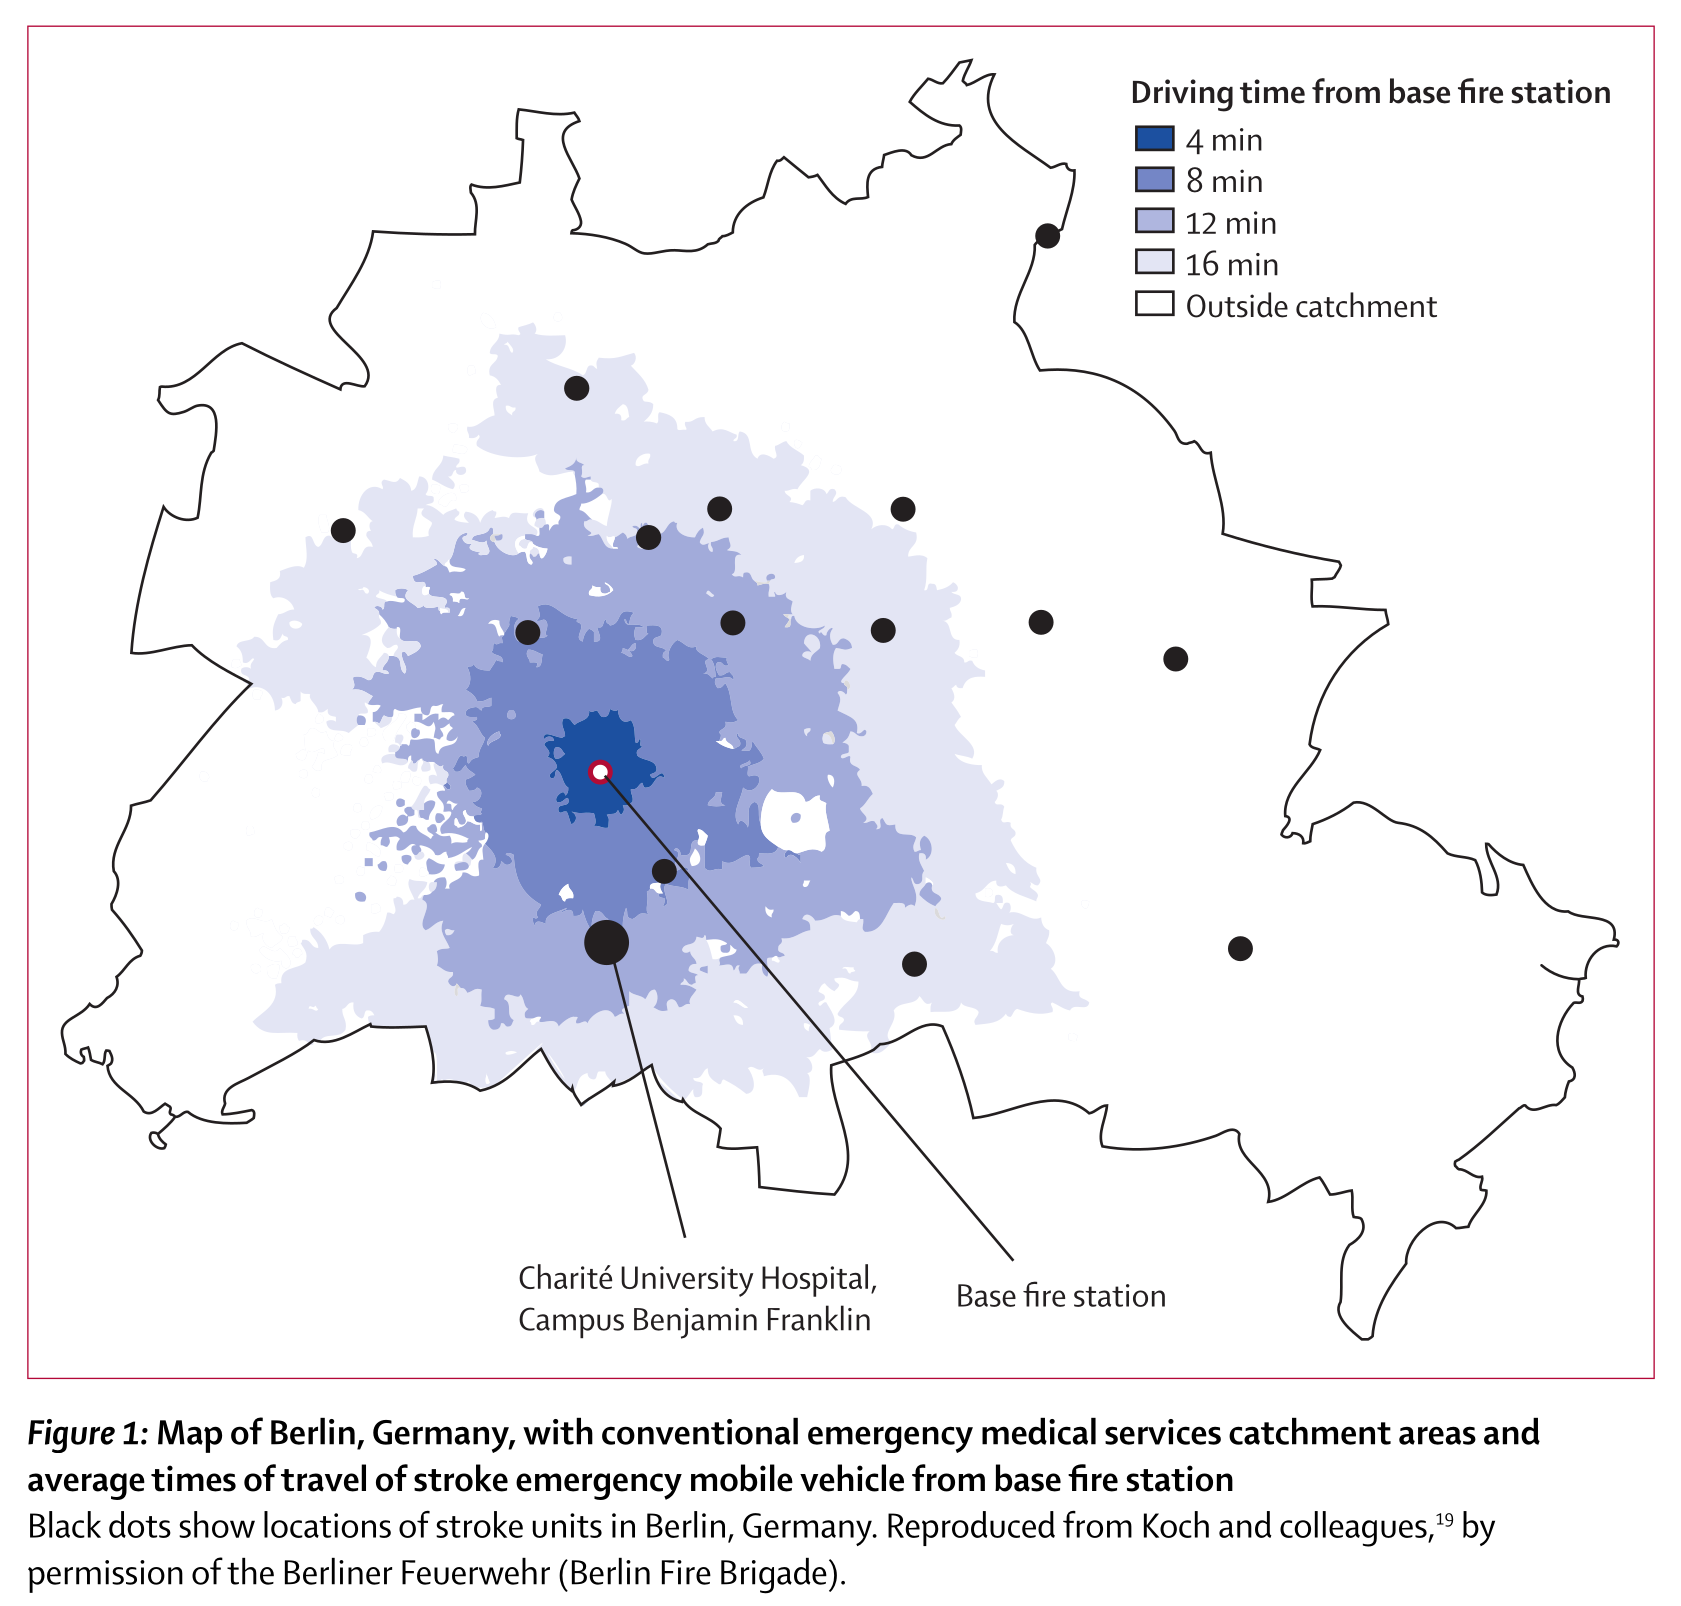
\includegraphics[width=0.5\linewidth]{images_background/berlin_map_1_.png}
    \caption{Map of Kunz et al. observational study area. MSU vs. care at the Charité Campus Benjamin Franklin in Berlin }
    \label{fig:map_berlin_1}
\end{figure}


\subsubsection{Ebinger et al., RCT, Berlin, 2021 Outcome trial \cite{ebinger_association_2021}}

\begin{markdown}
* Berlin, Germany
* Non-blind: Use a MSU if available (but not available for 44\% of calls)
* 1,543 patients (749 MSU, 794 normal care)
* Primary outcome: Distribution of mRS scores
\end{markdown}

Results (MSU vs. normal care, with IQR):

\begin{markdown}
* Lower median mRS at 3 months (mRS 1 vs 2)
* MSU had lower 3-month  disability scores: 80.3\% had none to moderate disability; 12.6\% had severe disability; and 7.1\% had died vs patients without an MSU dispatched: 78.0\% had none to moderate disability; 13..3\% had severe disability; and 8.8\% had died (common OR for worse functional outcome, 0.73, 95\% CI, 0.54-0.99; P = .04).
* Dispatch to MSU/ambo arrival (mins) 15 (12-19) vs 8 (6-10)
* Dispatch to hospital arrival (mins) 67 (46 to 82) vs 37 (31 to 44)
* Thrombolysis use: 60.2\% vs 48.1\%
* Thrombolysis dispatch to IVT mins: 50 (43 to 64) vs. 70 (59 to 86)
* Imaging to IVT: 12 (7 to 22) vs 15 (10 to 23)
* Door-to-needle (normal care) mins: 30 (22-40)
* Thrombectomy use: 13.8\% vs 14.2\%
* Dispatch to thrombectomy mins: 137 (117 to 166) vs 125 (110 to 154)
\end{markdown}

\subsubsection{Saarland, Germany, RCT, 2019, Helwig \cite{helwig_prehospital_2019}}

\begin{markdown}
* DESIGN, SETTING, AND PARTICIPANTS In this randomized multicenter trial with 3-month follow-up, patients were assigned week-wise to one of the pathways between June 15, 2015, and November 15, 2017, in 2 regions of Saarland, Germany; 708 of 824 suspected stroke patients did not meet inclusion criteria, resulting in a study population of 116 adult patients.

* INTERVENTIONS Patients received either OPM based on a standard operating procedure that included the use of the LAMS (cut point $>=$ 4) or management in an MSU (an ambulance with vascular imaging, point-of-care laboratory, and telecommunication capabilities). LAMS was used for hopsital selection. During the emergency call, the dispatcher screens patients for stroke symptoms. According to the study’s randomization plan, the dispatcher initiates either MSU-based stroke management or conventional stroke management optimized by the use of a preclinical stroke severity scale. Patients were enrolled in this trial after evaluation for inclusion and exclusion criteria and after written informed consent had been obtained. CONSORT indicates Consolidated Standards of Reporting Trials; CT, computed tomography; EMS, emergency medical services; ICU, intensive care unit; MSU, mobile stroke unit; and OPM, optimized prehospital management. 

* MAIN OUTCOMES AND MEASURES The primary end point was the proportion of patients accurately triaged to either CSCs (LVO, ICH) or PSCs (others). 

RESULTS A predefined interim analysis was performed after 116 patients of the planned 232 patients had been enrolled. Of these, 53 were included in the OPM group (67.9\% women; mean [SD] age, 74 [11] years) and 63 in the MSU group (57.1\% women; mean [SD] age, 75 [11] years). The primary end point, an accurate triage decision, was reached for 37 of 53 patients (69.8\%) in the OPM group and for 63 of 63 patients (100\%) in the MSU group (difference, 30.2\%; 95\% CI, 17.8\%-42.5\%; P < .001). Whereas 7 of 17 OPM patients (41.2\%) with LVO or ICH required secondary transfers from a PSC to a CSC, none of the 11 MSU patients (0\%) required such transfers (difference, 41.2\%; 95\% CI, 17.8\%-64.6\%; P = .02). The LAMS at a cut point of 4 or higher led to an accurate diagnosis of LVO or ICH for 13 of 17 patients (76.5\%; 6 triaged to a CSC) and of LVO selectively for 7 of 9 patients (77.8\%; 2 triaged to a CSC). Stroke management metrics were better in the MSU group, although patient outcomes were not significantly different.

\end{markdown}

Further results are given in figure \ref{fig:helwig_2019}. The eprformance of LAMs is shown in figure \ref{fig:helwig_lams}

\begin{figure}
    \centering
    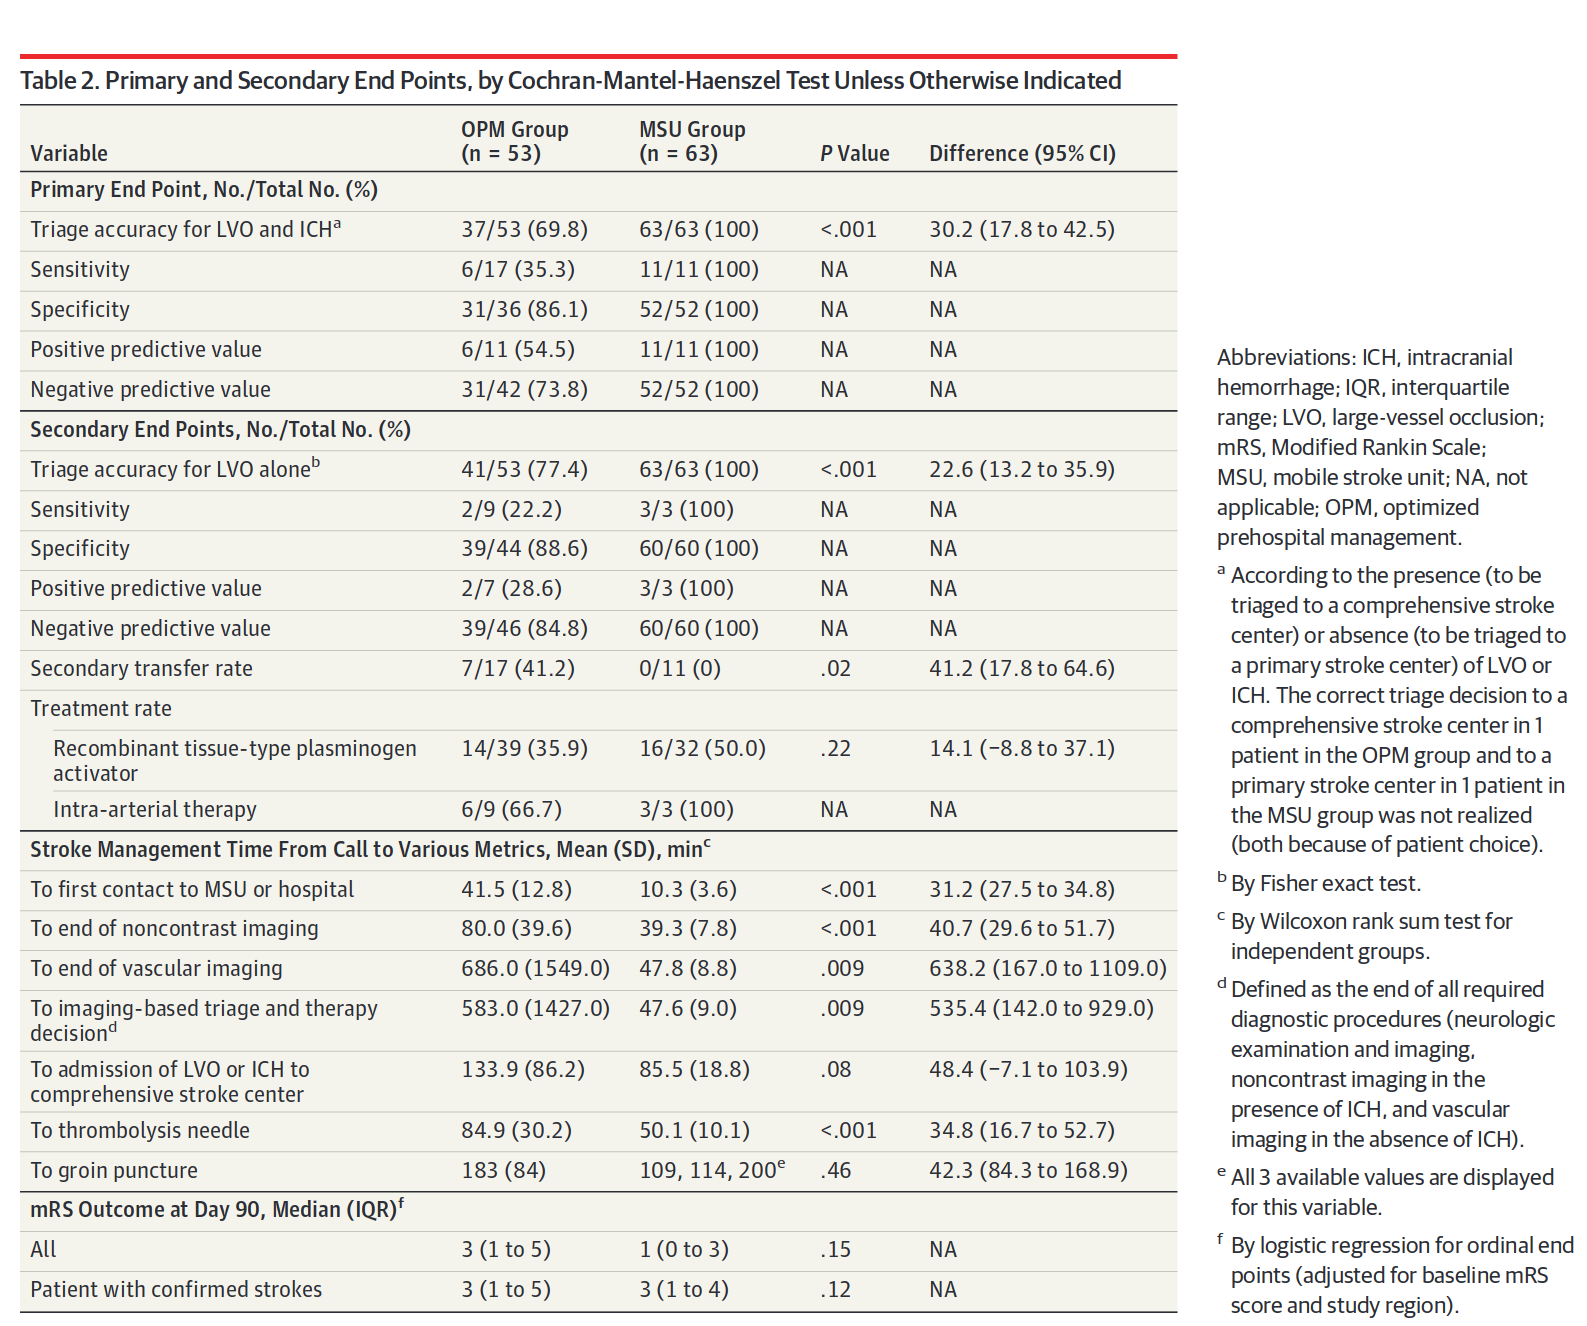
\includegraphics[width=0.95\linewidth]{images_background/helwig_2019.png}
    \caption{Results for Saarland trial \cite{helwig_prehospital_2019}}
    \label{fig:helwig_2019}
\end{figure}

\begin{figure}
    \centering
    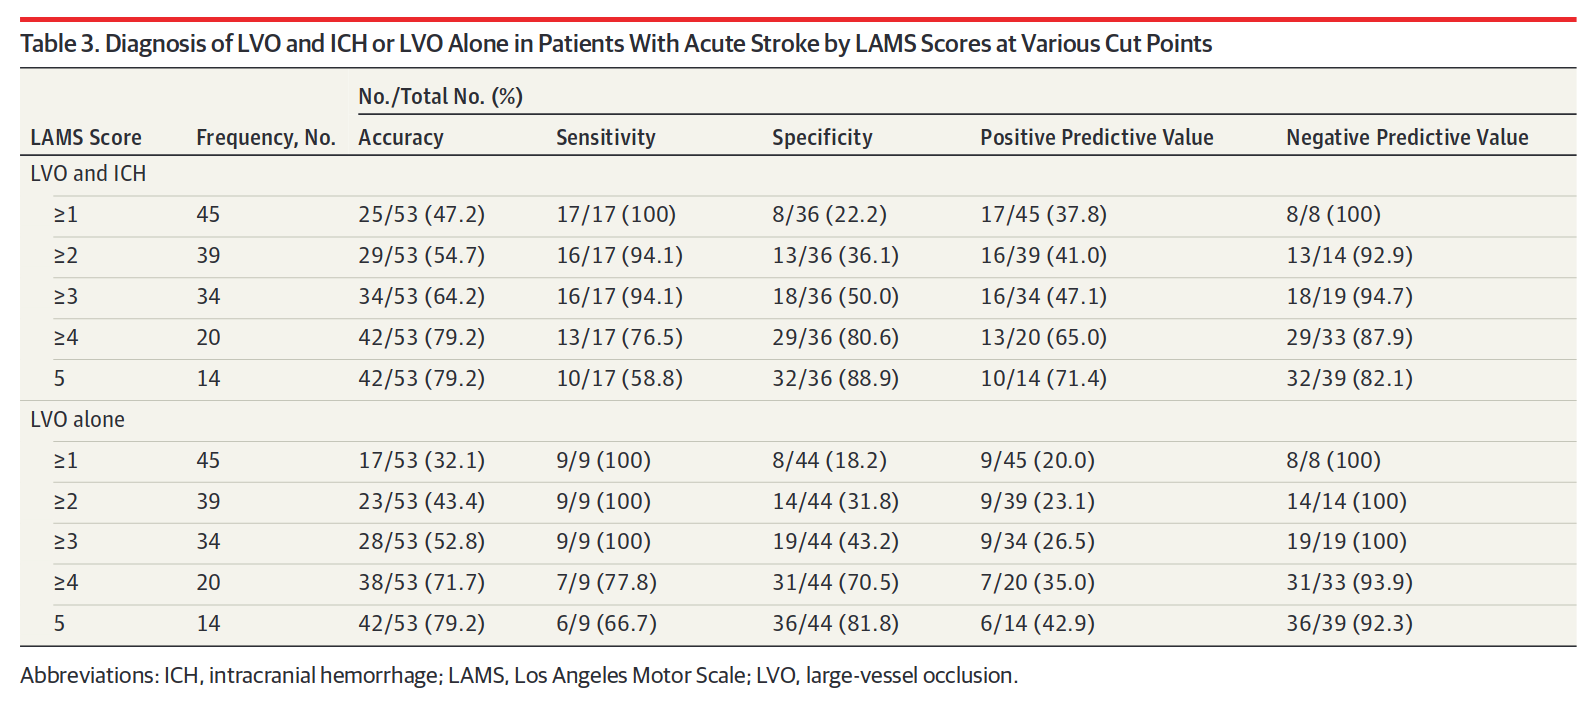
\includegraphics[width=0.95\linewidth]{images_background/helwig_lams.png}
    \caption{Results for performance of LAMS to identity LVO in Saarland trial \cite{helwig_prehospital_2019}}
    \label{fig:helwig_lams}
\end{figure}


\subsection{Individual trials - USA}

\subsubsection{Parker at al., RCT, Houston, US, 2015 \cite{parker_establishing_2015}}

\begin{markdown}
* Houston, Texas
* Pilot study to establish MSU
* Describes challenges in establishing MSU
\end{markdown}

\subsubsection{Borey et al., RCT, Houston, 2018 \cite{bowry_time_2018}}

Bowry et al \cite{bowry_time_2018} compared time from MSU arrival to decision in 50 patients in Houston. Time to tPA decision for the TM-VN was 21 minutes (interquartile range, 16.25–26) versus 18 minutes (interquartile range, 14–22) for the OB-VN (P=0.01). Initiation of tPA bolus was 24 minutes (interquartile range, 19.75–30) for the TM-VN versus 24 minutes (interquartile range, 19–27.75) for the OB-VN (P=0.5).


\subsubsection{BEST-MSU study, 7 US citiesd 2021 \cite{grotta_prospective_2021}}

Seven US cities:

1. Houston, Texas
2. Memphis, Tennessee  
3. Denver, Colorado
4. Los Angeles, California
5. New York, New York
6. Indianapolis, Indiana
7. Burlingame, California (San Mateo County)

Patients were considered to be enrolled if they met screening criteria for t-PA treatment on MSU or EMS arrival at the scene, whether or not they became eligible for the primary outcome analysis. Each MSU was staffed by one or two paramedics, a CT technologist, and a critical care nurse. A vascular neurology specialist supervised management on board or remotely through telemedicine, which have been shown to be similar in accuracy and speed.

The study enrolled 1515 patients, of whom 1047 were eligible to receive t-PA; 617 received care by MSU and 430 by EMS. The median time from onset of stroke to administration of t-PA was 72 minutes in the MSU group and 108 minutes in the EMS group. Of patients eligible for t-PA, 97.1\% in the MSU group received t-PA, as compared with 79.5\% in the EMS group. The mean score on the utility-weighted modified Rankin scale at 90 days in patients eligible for t-PA was 0.72 in the MSU group and 0.66 in the EMS group (adjusted odds ratio for a score of $\ge$ 0.91, 2.43; 95\% confidence interval [CI], 1.75 to 3.36; P<0.001). Among the patients eligible for t-PA, 55.0\% in the MSU group and 44.4\% in the EMS group had a score of 0 or 1 on the modified Rankin scale at 90 days. Among all enrolled patients, the mean score on the utility-weighted modified Rankin scale at discharge was 0.57 in the MSU group and 0.51 in the EMS group (adjusted odds ratio for a score of  $\ge$ 0.91, 1.82; 95\% CI, 1.39 to 2.37; P<0.001). Secondary clinical outcomes generally favored MSUs. Mortality at 90 days was 8.9\% in the MSU group and 11.9\% in the EMS group.

The BEST Study \cite{grotta_prospective_2021} timings are shown in figure \ref{fig:best_msu_timings}. For EMS, derived process times are: call-to-ambo = 9 min, ambo on-scene and travel time to ED = 27 min, ED arrival-to-IVT = 40 min. For MSU timings are call-to-ambo = 9 min. MSU arrival to IVT = 35 min, ambo on-scene and travel time to ED = 55 min. The median (and IQR) time from 911 alert to \textbf{thrombectomy} was 141 (116–171) and 132 minutes (114–160) for MSU and EMS, and  time from ED door to thrombectomy was 76 (53–105) and 94 (72–124). Note - these patients call 911 soon after stroke. MSUs improve time to thrombolysis, but slow time to arrival at ED. Overall onset to thrombectomy times are similar (slower arriving at ED, but faster arrival-to-thrombectomy times). 

\begin{figure}
    \centering
    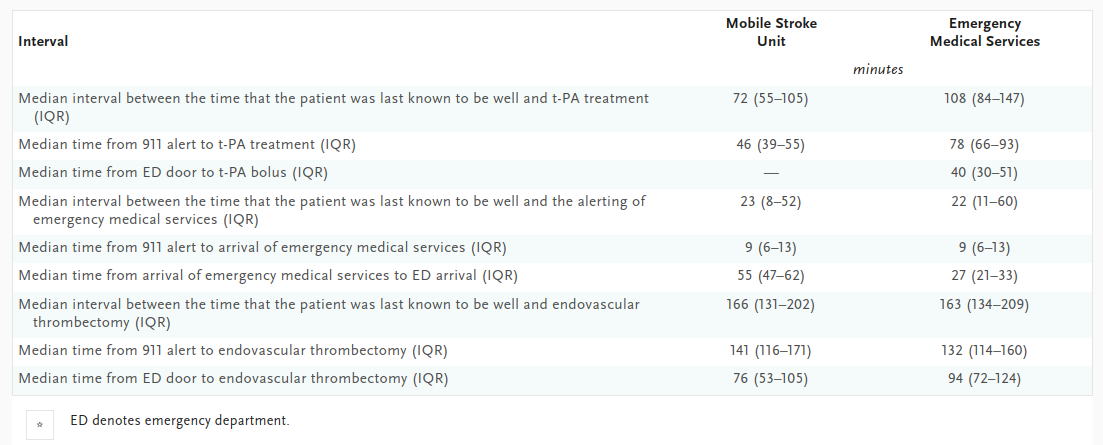
\includegraphics[width=0.75\linewidth]{images_background/best_msu_timings.png}
    \caption{BEST-MSU Timings}
    \label{fig:best_msu_timings}
\end{figure}


\subsubsection{Cleveland, Taqui, RCT, 2017 \cite{taqui_reduction_2017}}

\begin{markdown}
* Telemedicine-equipped MSU vs normal care
* Cleveland, Ohio
* The evaluation and treatment of the first 100 MSTU patients (July 18, 2014–November 1, 2014) was compared to a control group of 53 patients brought to the ED via a traditional ambulance in 2014. 
* Times are expressed as medians with their interquartile ranges
* Results: Patient and stroke severity characteristics were similar between 100 MSTU and 53 ED control patients (initial NIH Stroke Scale score 6 vs 7, p 5 0.679). There was a significant reduction of median alarm-to-CT scan completion times (33 minutes MSTU vs 56 minutes controls, p $<$ 0.0001), median alarm-to-thrombolysis times (55.5 minutes MSTU vs 94 minutes controls, p , 0.0001), median door-to-thrombolysis times (31.5 minutes MSTU vs 58 minutes controls, p = 0.0012), and symptom-onset-to-thrombolysis times (97 minutes MSTU vs 122.5 minutes controls, p 5 0.0485). Sixteen patients evaluated on MSTU received thrombolysis, 25\% of whom received it within 60 minutes of symptom onset.
* Of the 100 MSU evaluations, 33 were probable ischaemic stroke (16 given thrombolysis), 30 were possible ischaemic stroke (no thrombolysis), 4 were TIA, 5 were ICH, and 28 were noncerebrovascular.
   
\end{markdown}

Further results are shown in figure \ref{fig:taqi_2017}

\begin{figure}
    \centering
    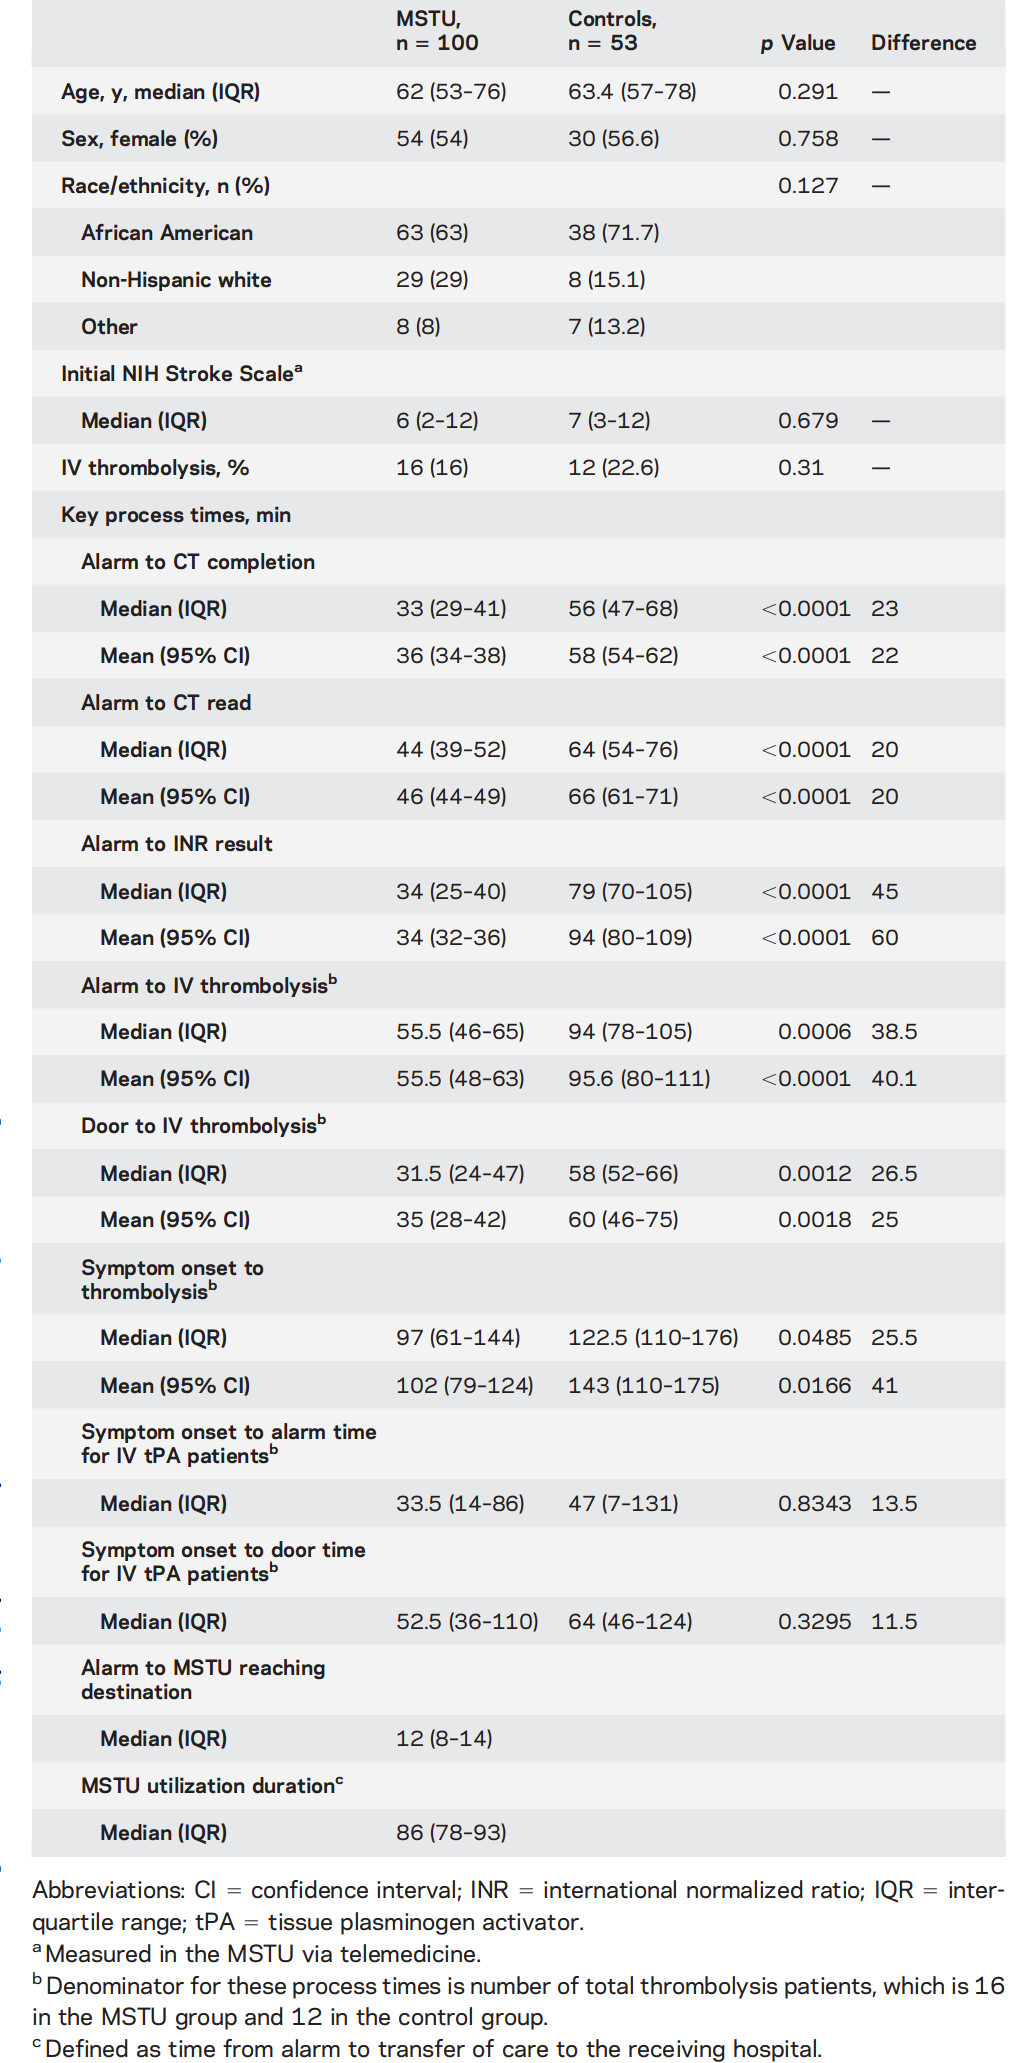
\includegraphics[width=0.65\linewidth]{images_background/taqi_2017.png}
    \caption{Results fot Taqi et al \cite{taqui_reduction_2017}}
    \label{fig:taqi_2017}
\end{figure}

\subsubsection{New York, Kummer, Observationalo study, 2019, \cite{kummer_geographic_2019}}

\begin{markdown}
* Analysis of New York registry
* bi-institutional MSU operating in Manhattan, New York, from October 2016 to September 2017. The comparison group included patients transported to our hospitals via conventional ambulance for acute ischemic stroke during the same hours of MSU operation (Monday to Friday, 9 AM to 5 PM).
* We identified 66 patients treated or transported by MSU and 19 patients transported by conventional ambulance. Patients receiving MSU care had significantly shorter dispatch-to-thrombolysis time than patients receiving conventional care (mean: 61.2 versus 91.6 minutes; P=0.001). Compared with patients receiving conventional care, patients receiving MSU care were significantly more likely to be picked up closer to a higher mean number of designated stroke centers in a 2.0-mile radius (4.8 versus 2.7, P=0.002). In multivariable analysis, MSU care was associated with a mean decrease in dispatch-tothrombolysis time of 29.7 minutes (95\% CI, 6.9–52.5) compared with conventional care.
* Possible issue here is MSU biased towards normal day care times which may skew results.
\end{markdown}

\subsubsection{BEST-MSU substudy on pre-stroke disability \cite{pirlog_outcomes_2023}}

\textbf{Background}: Few data exist on acute stroke treatment in patients with pre-existing disability (PD) since they are usually excluded from clinical trials. A recent trial of mobile stroke units (MSUs) demonstrated faster treatment and improved outcomes, and included PD patients.

\textbf{Aim}: To determine outcomes with tissue plasminogen activator (tPA), and benefit of MSU versus management by emergency medical services (EMS), for PD patients.

\textbf{Methods}: Primary outcomes were utility-weighted modified Rankin Scale (uw-mRS). Linear and logistic regression models compared outcomes in patients with versus without PD, and PD patients treated by MSU versus standard management by EMS. Time metrics, safety, quality of life, and health-care utilization were compared.

\textbf{Results}: Of the 1047 tPA-eligible ischemic stroke patients, 254 were with PD (baseline mRS 2-5) and 793 were without PD (baseline mRS 0-1). Although PD patients had worse 90-day uw-mRS, higher mortality, more health-care utilization, and worse quality of life than non-disabled patients, 53\% returned to at least their baseline mRS, those treated faster had better outcome, and there was no increased bleeding risk. Comparing PD patients treated by MSU versus EMS, 90-day uw-mRS was 0.42 versus 0.36 (p = 0.07) and 57\% versus 46\% returned to at least their baseline mRS. There was no interaction between disability status and MSU versus EMS group assignment (p = 0.67) for 90-day uw-mRS.

\textbf{Conclusion}: PD did not prevent the benefit of faster treatment with tPA in the BEST-MSU study. Our data support inclusion of PD patients in the MSU management paradigm.

%%%%%%%%%%%%%%%%%%%%%%%%%%%%%%%%%%%%%%%%%% TELEMEDICINE %%%%%%%%%%%%%%%%%%%%%%%%%%%%%%%%%%%%%%%%%%
\subsection{MSU Telemedicine}

In a study of 174 patients in Houston, telemedicine neurologist assessment for a mobile stroke unit was reliable and fast \cite{wu_telemedicine_2017} . tPA decisions agreed 88\% of the time. NIHSS correlated well (0.88). Overall, there was disagreement in 20 of the 170 cases with decisions. In 13 out of 20 cases, the onboard vascular neurologist recommended tPA, whereas the telemedicine vascular neurologist did not. In 7 out of 20 cases, the telemedicine vascular neurologist recommended tPA whereas the onboard vascular neurologist did not. 

Bowry et al \cite{bowry_time_2018} compared time to decision in 50 patients in Houston. Time to tPA decision for the TM-VN was 21 minutes (interquartile range, 16.25–26) versus 18 minutes (interquartile range, 14–22) for the OB-VN (P=0.01). Initiation of tPA bolus was 24 minutes (interquartile range, 19.75–30) for the TM-VN versus 24 minutes (interquartile range, 19–27.75) for the OB-VN (P=0.5).

\subsection{Staffing of Mobile Stroke units}

\subsubsection{USA BEST-MSU Study}

From [2]: Onboard staff typically includes emergency medical technicians or paramedics, a radiology technician, and nurse or nurse practitioner, in addition to a vascular neurologist.4 Some variants, such as that of the Cleveland Clinic, employ telemedicine consultation with the vascular neurologist. 

1. Emergency medical technicians (EMTs) or paramedics[2]
2. A radiology technician[2]
3. A nurse or nurse practitioner[2]
4. A vascular neurologist (either on-board or via telemedicine)[2][4]

Some key points about the staffing:

- The vascular neurologist could be physically present on the MSU or provide consultation via telemedicine, depending on the specific setup[2][4].

- The Cleveland Clinic variant of the MSU employed telemedicine consultation with the vascular neurologist rather than having them physically on board[2].

- Dr. Grotta's team demonstrated that assessment done through telemedicine was just as reliable as that of an on-board vascular neurologist[2].

- The MSU was equipped to function like a "primary stroke center emergency department on wheels" with this specialized team and resources to diagnose stroke and begin treatment before arriving at the hospital[6].

This staffing model allowed the MSU to provide clinical assessment, imaging diagnosis, and hyperacute treatment in the field, significantly reducing time to treatment for stroke patients compared to traditional emergency medical services[4][6].

Citations:
[1] https://pubmed.ncbi.nlm.nih.gov/26508753/
[2] https://practicalneurology.com/articles/2018-jan/mobile-stroke-units
[3] https://www.urmc.rochester.edu/stroke-center/mobile-stroke/about-msu/msu-q-a.aspx
[4] https://www.ncbi.nlm.nih.gov/pmc/articles/PMC9240459/
[5] https://pubmed.ncbi.nlm.nih.gov/34496173/
[6] https://www.uclahealth.org/news/article/new-study-shows-mobile-stroke-units-lead-to-better-patient-outcomes

\subsubsection{Berlin \cite{ebinger_effects_2015}}

* The MSU was staffed with a neurologist trained in emergency medicine, a
paramedic, and a radiology technician. A neuroradiologist was on call to evaluate images acquired on board the STEMO via a teleradiology connection.



%%%%%%%%%%%%%%%%%%%%%%%%%%%%%%%%%%%%%%%%%% THROMBECTOMY %%%%%%%%%%%%%%%%%%%%%%%%%%%%%%%%%%%%%%%%%%

\subsection{MSUs and thrombectomy}

The BEST-MSU substudy \cite{czap_abstract_2022} was a subset of the best MSU study, for tPA-eligible stroke patients with LVOs on CT and/or CTA. The study appeared to show MSUs have little effect on time to thrombectomy. A total of 295 patients were included, 169 in the MSU group and 126 in the EMS group. 92\% MSU vs 87\% EMS LVO patients received tPA, and 78\% vs 85\% went on to have EVT. MSU LVO patients had faster tPA bolus from symptom onset (65 min vs 96 min, p<0.001), however the two groups had similar onset to groin puncture (169 min vs 162 min, p=0.77). From the BEST study \cite{grotta_prospective_2021}, the median (and IQR) time from 911 alert to  thrombectomy was 141 (116–171) and 132 minutes (114–160) for MSU and EMS, and  time from ED door to thrombectomy was 76 (53–105) and 94 (72–124).

The Berlin study \cite{ebinger_association_2021} had MSU vs nomral care:

* Thrombectomy use: 13.8\% vs 14.2\%
* Dispatch to thrombectomy mins: 137 (117 to 166) vs 125 (110 to 154)


The Melbourne MSU study \cite{menezes_abstract_2023} found MSUs improved thrombectomy use and speed during, but not before, the COVID pandemic. A total of 402 patients (112 MSU) were included. Pre-pandemic, no reduction in dispatch to arterial access time was seen for MSU patients within an EVT centre catchment (median 11 min slower, p=0.38). However, a significant time saving was observed during the pandemic (median 29 min faster, p<0.001, p=0.0065). MSU care reduced hospital arrival to arterial access time by median 19 min pre-pandemic vs 40 min during the pandemic, p<0.001).

In Sydney the MSU did not improve time or rate of thrombectomy \cite{haliem_abstract_2023} but the MSU dispatch missed 40\% of those patients that would go on to receive thrombectomy. An odd finding there was also the ambo dispatch process was less likely to class severe strokes as stroke, compared to mild stroke. A total of n=618 patients were included with baseline NIHSS 16 (IQR 10-20). Of these, only 62\% (95\% CI 58-66) were initially dispatched as suspected stroke, with the most common non-stroke diagnoses being “Unconscious/Fainting” (19.2\%) and “Falls” (6.9\%). Those with a higher baseline severity (NIHSS $\ge$ 10) were less likely to be classified as stroke than those with lower severity (59\% vs 76\%, p<0.001), while no difference was found between metropolitan and rural patients (p=0.066). Overall, no significant time differences were found between stroke and non-stroke dispatches for ambulance dispatch to arterial access (median 208 vs 216 min, p=0.593) or hospital arrival to arterial access (median 42 vs 42 min, p=0.851). However, only 32 patients were treated on the MSU, which commenced operation November 2017 (2007-2021 was used for all data analysis). 

In Saarland \cite{helwig_prehospital_2019} time from call to puncture was 183 mins (SD 84) in the control group and 141 mins in the MSU group, but there were only 3 thrombectomy patients in the MSU group


A review of available evidence suggests there is an evidence gap in MSUs and thrombectomy \cite{navi_mobile_2022}.

\subsection{Benefit of redirection}

Romoli et al. \cite{romoli_mothership_2020} reviewed evidence on mothership vs drip and ship. 

\textbf{Background and Purpose} : Substantial uncertainty exists on the benefit of organizational paradigms in stroke networks. Here we systematically reviewed and meta-analyzed data from studies comparing functional outcome between the mothership (MS) and the drip and ship (DS) models.

\textbf{Methods}: The meta-analysis protocol was registered international prospective register of systematic reviews (PROSPERO) and followed Preferred Reporting Items for Systematic Reviews and Meta-Analyses (PRISMA) guidelines. PubMed, EMBASE, and Cochrane Central databases were searched for randomized-controlled clinical trials (RCTs), retrospective and prospective studies comparing MS versus DS. Primary endpoints were functional independence at 90 days (modified Rankin Scale <3) and successful recanalization (Thrombolysis in Cerebral Infarction Scale [TICI] >2a); secondary endpoints were 3-month mortality and symptomatic intracranial haemorrhage (sICH). Odds ratios for endpoints were pooled using the random effects model and were compared between the two organizational models.

\textbf{Results}:  Overall, 18 studies (n=7,017) were included in quantitative synthesis. MS paradigm was superior to DS model for functional independence (odds ratio, 1.34; 95\% confidence interval, 1.16 to 1.55;). Meta-regression analysis revealed association between onset-to-needle time and good functional outcome, with longer onset-to-needle time being detrimental. Similar rates of recanalization, sICH and mortality at 90 days were documented between MS and DS.

\textbf{Conclusions}: Patients with acute ischemic stroke eligible for reperfusion strategies might benefit more from MS paradigm as compared to DS. RCTs are needed to further refine best management taking into account logistics, facilities and resources.



%%%%%%%%%%%%%%%%%%%%%%%%%%%%%%%%%%%%%%%%%% PICTURES %%%%%%%%%%%%%%%%%%%%%%%%%%%%%%%%%%%%%%%%%%

\begin{figure}
    \centering
    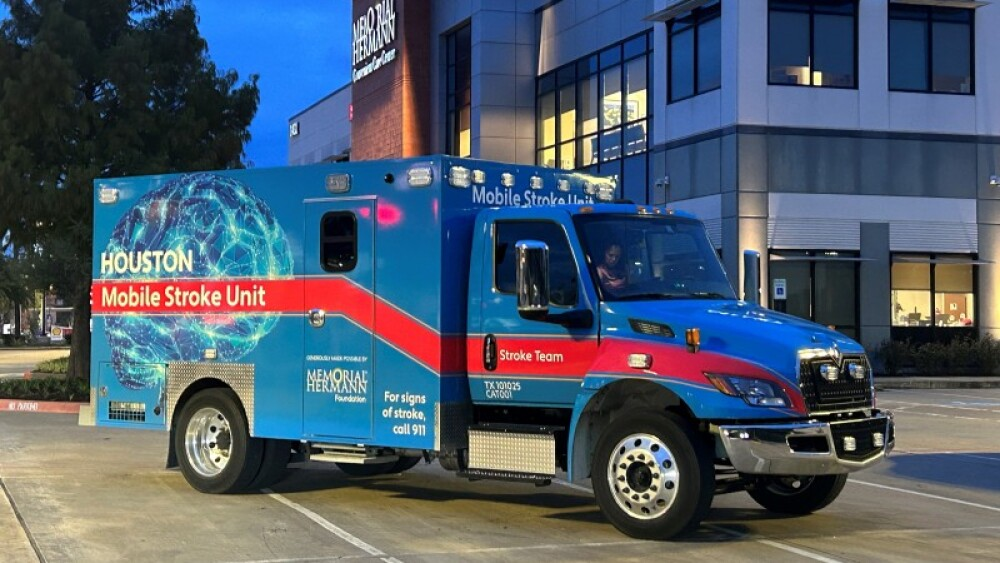
\includegraphics[width=0.5\linewidth]{images_background/houston_msu.jpeg}
    \caption{Houston Mobile Stroke Unit}
    \label{fig:houston_msu}
\end{figure}

\printbibliography[title={References for supplementary material}]
%TC:endignore
\end{refsection}


\end{document}